% concatenated from arixvflexibilityofnilfactors.tex
\documentclass[12pt]{amsart}
\usepackage{graphicx} % Required for inserting images
\usepackage{fancyhdr}



\title{Flexibility of measurable and topological nilfactors in dynamical systems}
\author{Seljon Akhmedli}
\thanks{The author was partially supported by NSF grant DMS-2136217}

\address{Department of Mathematics, Northwestern University}
\email{seljonakhmedli2026@u.northwestern.edu}

\title[Flexibility of nilfactors in dynamical systems]{Flexibility of measurable and topological nilfactors in dynamical systems}

\usepackage{amsmath, amssymb, mathrsfs}
\usepackage{mathpazo}
\usepackage{latexsym,array,delarray,amsthm,amssymb,epsfig,setspace,tikz,amsmath,enumerate,mathrsfs,graphicx, mathtools,cite}

\usepackage{tabularx}
\usepackage{tikz-cd}
\usepackage{tikz}
\usepackage{floatrow}
\usepackage{hyperref}
\usetikzlibrary{positioning}
\usepackage{comment}
\usepackage{amsthm}
\usepackage{arydshln}


\newtheorem{fact}{Fact}


\usepackage{geometry}\geometry{margin=1.45in}

\renewcommand{\labelenumi}{\arabic{enumi}.}
\renewcommand{\labelenumii}{\alph{enumii}.}



% environments
\newtheorem{thm}{Theorem}[section]
\newtheorem{lem}[thm]{Lemma}
\newtheorem{prop}[thm]{Proposition}
\theoremstyle{definition}
\newtheorem{defn}[thm]{Definition}
\newtheorem{exmp}[thm]{Example}
\newtheorem{rem}[thm]{Remark}
\newtheorem{cor}[thm]{Corollary}
\newtheorem{question}[thm]{Question}

\newcommand{\Diff}{\mathop{\rm Diff}}
\newcommand{\Homeo}{\mathop{\rm Homeo}}
\newcommand{\Fix}{\mathop{\rm Fix}}
\newcommand{\supp}{\mathop{\rm supp}}


\newcommand{\blackboard}[1]{\ensuremath{\mathbb{#1}}}
\newcommand{\script}[1]{\ensuremath{\mathcal{#1}}}
\newcommand{\smallcaps}[1]{\ensuremath{\textsc{#1}}}
\newcommand{\N}{\blackboard{N}}
\newcommand{\pos}{\blackboard{P}}
\newcommand{\Z}{\blackboard{Z}}
\newcommand{\Zodd}{\blackboard{Z}_{\textrm{odd}}}
\newcommand{\Q}{\blackboard{Q}}
\newcommand{\R}{\blackboard{R}}
\newcommand{\C}{\blackboard{C}}
\newcommand{\X}{\blackboard{X}}
\newcommand{\A}{\blackboard{A}}
\newcommand{\F}{\ensuremath{\mathbf{F}}}
\newcommand{\free}{\smallcaps{Free}}

%\usepackage{makeidx}
\makeindex
\def\lbr{\left\{}
\def\rbr{\right\}}

\def\msg{{\mathscr G}}
\def\msk{{\mathscr K}}
\def\msb{{\mathscr B}}
\def\msd{{\mathscr D}}
\def\mso{{\mathscr O}}
\def\msa{{\mathscr A}}
\def\mss{{\mathscr S}}
\def\msf{{\mathscr F}}
\def\msh{{\mathscr H}}
\def\msl{{\mathscr L}}
\def\msp{{\mathscr P}}
\def\msc{{\mathscr C}}
\def\mst{{\mathscr T}}
\def\msm{{\mathscr M}}
\def\msi{{\mathscr I}}
\def\msn{{\mathscr N}}
\def\cE{{\mathcal E}}
\def\cF{{\mathcal F}}
\def\cB{{\mathcal B}}
\def\cC{{\mathcal C}}
\def\cH{{\mathcal H}}
\def\cP{{\mathcal P}}
\def\cN{{\mathcal N}}
\def\cR{{\mathcal R}}
\def\cI{{\mathcal I}}
\def\cG{{\mathcal G}}
\def\cA{{\mathcal A}}
\def\mh{{\mathbb  H}}
\def\mq{{\mathbb  Q}}
\def\me{{\mathbb  E}}
\def\mb{{\mathbb  B}}
\def\mr{{\mathbb  R}}
\def\mm{{\mathbb  M}}
\def\mn{{\mathbb  N}}
\def\mz{{\mathbb  Z}}
\def\ms{{\mathbb  S}}
\def\mp{{\mathbb  P}}
\def\mi{{\mathbb I}}
\newcommand{\rf}[1]{(\ref{#1})}
\def\lnfrac#1#2{\raise.7ex \hbox{\Small $#1$}%%
  \kern-.15em/\kern-.15em  \lower.2ex \hbox{\Small $#2$}}


\theoremstyle{plain}
\newtheorem{theorem}{Theorem}[section]
\newtheorem{corollary}[theorem]{Corollary}
\newtheorem{lemma}[theorem]{Lemma}
\newtheorem{proposition}[theorem]{Proposition}
\newtheorem{definition}[theorem]{Definition}

\theoremstyle{definition}
\newtheorem{exercise}[theorem]{Exercise}
\newtheorem{example}[theorem]{Example}
\newtheorem{remark}[theorem]{Remark}
\newtheorem{claim}[theorem]{Claim}

\pagenumbering{arabic}

%\newcounter{chsec}
\def\thechsec{{\thechapter}.{\thesection}}
\numberwithin{equation}{section}
%\numberwithin{theorem}{chsec}
%comment out next line if not want chapter numbers
%\numberwithin{section}{chapter}
%\numberwithin{equation}{chapter}

\usepackage{setspace}

\begin{document}

\begin{comment}

Nilsystems have arisen in various contexts both in ergodic theory and topological dynamics. Their standard properties have, for instance, been studied in \cite{Auslander} and \cite{Parry}. 

Given a minimal and ergodic system, we can discuss both measurable and topological properties. 

Every topological factor can be viewed as a measurable factor, but the converse is not always true. In fact, for the measurable and topological nilfactors this is precisely what determines when they are isomorphic or not(see for example... point out lemma).

Given a minimal and ergodic system, we can discuss both its measurable and topological nilfactors. 
We construct examples of strictly ergodic systems realizing all possible behaviors in the interplay of measurable and topological nilfactors. To build such examples, we adapt on an idea that stems from Furstenberg's construction of a minimal but not uniquely ergodic system on $\mathbb{T}^2$.

\end{comment}

\begin{abstract}
%Given a minimal and ergodic system, we can discuss both its measurable and topological nilfactors. 
We construct examples of minimal and uniquely ergodic systems realizing all possible behaviors in the interplay of measurable and topological nilfactors. To build such examples, we adapt an idea that stems from Furstenberg's construction of a minimal but not uniquely ergodic system on $\mathbb{T}^2$.
%For each $k\geq 1$, we construct examples of strictly ergodic systems $(X,\mu,T)$ where the maximal measurable and topological $i$-step nilfactors of $X$ are topologically isomorphic for $0 \leq i \leq j$, but they are \textit{not} measurably isomorphic for $j+1 \leq i \leq k$, where $0 \leq j \leq k$. In doing so, for all $\ell$ with $j \leq \ell \leq k$, we can arrange the maximal topological $\ell$-step nilfactor to be topologically isomorphic to the maximal topological $i$-step nilfactor for all $i\geq \ell$. This captures all possible behaviors in the interplay of measurable and topological nilfactors. 






%with %$X$ being a compact metric space, $T$ a homeomorphism of $X$, and $\mu$ a $T$-invariant Borel probability measure,
%its maximal measurable $k$-step nilfactor is denoted by $Z_k$ and its topological analog by $X_k$. %In many of the examples given, $Z_k$ is measurably isomorphic to $X_k$ for all $k \in \mathbb{N}$. 
%In this paper, for each $k \geq 1$, we construct examples of strictly ergodic systems where $Z_i$ and $X_i$ are topologically isomorphic for $0 \leq i \leq j$, but $Z_i$ and $X_i$ are \textit{not} measurably isomorphic for $j+1 \leq i \leq k$, where $0 \leq j \leq k$. 
%In doing so, for all $\ell$ with $j \leq \ell \leq k$, we can arrange $X_i$ to be topologically isomorphic to $X_\ell$ for all $i\geq \ell$. This captures all possible behaviors in the interplay of measurable and topological nilfactors. 
%Given a minimal and ergodic dynamical system $(X,\mu,T)$, %with %$X$ being a compact metric space, $T$ a homeomorphism of $X$, and $\mu$ a $T$-invariant Borel probability measure,
%its maximal measurable $k$-step nilfactor is denoted by $Z_k$ and its topological analog by $X_k$. %In many of the examples given, $Z_k$ is measurably isomorphic to $X_k$ for all $k \in \mathbb{N}$. 
%In this paper, for each $k \geq 1$, we construct examples of strictly ergodic systems where $Z_i$ and $X_i$ are topologically isomorphic for $0 \leq i \leq j$, but $Z_i$ and $X_i$ are \textit{not} measurably isomorphic for $j+1 \leq i \leq k$, where $0 \leq j \leq k$. 
%In doing so, for all $\ell$ with $j \leq \ell \leq k$, we can arrange $X_i$ to be topologically isomorphic to $X_\ell$ for all $i\geq \ell$. This captures all possible behaviors in the interplay of measurable and topological nilfactors. 
\end{abstract}

%\newcommand{\dasharrow}{%
 % \tikz[baseline=-0.5ex]{%
  %  \draw[dashed,->] (0,0) -- (1.2em,0);
 % }%
%}

\newcommand{\dash}{\tikz[baseline=-0.7ex]{\draw[dashed] (0,0) -- (1.3em,0);}}



\renewcommand{\labelenumi}{\arabic{enumi}.}
\renewcommand{\labelenumii}{\alph{enumii}.}




\def\lbr{\left\{}
\def\rbr{\right\}}

\def\msg{{\mathscr G}}
\def\msk{{\mathscr K}}
\def\msb{{\mathscr B}}
\def\msd{{\mathscr D}}
\def\mso{{\mathscr O}}
\def\msa{{\mathscr A}}
\def\mss{{\mathscr S}}
\def\msf{{\mathscr F}}
\def\msh{{\mathscr H}}
\def\msl{{\mathscr L}}
\def\msp{{\mathscr P}}
\def\msc{{\mathscr C}}
\def\mst{{\mathscr T}}
\def\msm{{\mathscr M}}
\def\msi{{\mathscr I}}
\def\msn{{\mathscr N}}
\def\cE{{\mathcal E}}
\def\cF{{\mathcal F}}
\def\cB{{\mathcal B}}
\def\cC{{\mathcal C}}
\def\cH{{\mathcal H}}
\def\cP{{\mathcal P}}
\def\cN{{\mathcal N}}
\def\cR{{\mathcal R}}
\def\cI{{\mathcal I}}
\def\cG{{\mathcal G}}
\def\cA{{\mathcal A}}
\def\mh{{\mathbb  H}}
\def\mq{{\mathbb  Q}}
\def\me{{\mathbb  E}}
\def\mb{{\mathbb  B}}
\def\mr{{\mathbb  R}}
\def\mm{{\mathbb  M}}
\def\mn{{\mathbb  N}}
\def\mz{{\mathbb  Z}}
\def\ms{{\mathbb  S}}
\def\mp{{\mathbb  P}}
\def\mi{{\mathbb I}}

\pagenumbering{arabic}

%\newcounter{chsec}
\def\thechsec{{\thechapter}.{\thesection}}
\numberwithin{equation}{section}
%\numberwithin{theorem}{chsec}
%comment out next line if not want chapter numbers
%\numberwithin{section}{chapter}
%\numberwithin{equation}{chapter}



\maketitle

\section{Introduction}

Nilsystems and nilfactors of systems arise in convergence and recurrence problems in ergodic theory and topological dynamics. Prime examples of these can be found in \cite{topological characteristic factors} and \cite{HK paper}. Numerous measure-theoretic and topological properties, such as transitivity, minimality, ergodicity, and unique ergodicity, are equivalent in nilsystems, combining results of \cite{Auslander, Leibman, Lesigne, Parry2}. These equivalences are key in many recent developments in dynamics. 

To describe the behaviors that may arise, we assume throughout that our dynamical systems are endowed with both measurable and topological structure. %allowing us to discuss both measurable and topological factors. %Thus we assume that $(X,\mu,T)$ is a minimal and ergodic system, meaning $X$ is a compact metric space, $T$ is a minimal homeomorphism of $X$, and $\mu$ is a $T$-invariant ergodic Borel probability measure. 
Every topological factor naturally has the structure of a measurable factor, but the converse does not hold in general. %In fact, for the measurable and topological nilfactors, this precisely determines when they are isomorphic or not. 

The measurable $k$-step nilfactor of a system has been shown in works of Host and Kra in \cite{HK paper} to control the dynamical behavior of certain multiple ergodic averages. The topological analog of these factors was first introduced by Host, Kra and Maass in \cite{Host Kra and Maass} (see Section \ref{sec: notations and preliminaries} for definitions). A more recent interplay of the measurable and topological nilfactors has appeared in \cite{a model with topological pronilfactors} where Kra, Moreira, Richter and Robertson, solved a conjecture of Erd\H{o}s on sumsets. There, it was shown how these nilfactors control certain infinite patterns in sets with positive density. %Nilsystems are classic examples where the measurable and topological nilfactors, $Z_k$ and $X_k$, are isomorphic. 

The well-known Jewett-Krieger theorem says that every ergodic system has a strictly ergodic (minimal and uniquely ergodic) topological model \cite{{Jewett}, {Krieger}}. By a topological model, or just model, we mean a topological dynamical system equipped with an invariant probability measure that is measurably isomorphic to the original system.
In \cite{maximal pronilfactors}, it is shown that every ergodic system has a strictly ergodic model where the measurable and topological $k$-step nilfactors, $Z_k$ and $X_k$, are isomorphic. An older result of Lehrer \cite{Lehrer} obtaining topologically mixing models of ergodic systems is most relevant for this work. An important consequence of his theorem is the existence of systems where $Z_1$ and $X_1$ are not isomorphic; it then follows $Z_i$ and $X_i$ are not isomorphic as well for all $i>1$. Concrete examples of such systems can be found in, for instance, \cite{{nontrivial Kronecker trivial MEF}, {Gla}, {Lehrer}, {Parry}}. %Obtaining additionally topologically mixing models of ergodic systems is an older result of Lehrer \cite{Lehrer} which is most relevant for this work. An important consequence of his theorem is the existence of systems where $Z_1$ and $X_1$ are not isomorphic; it then follows $Z_i$ and $X_i$ are not isomorphic as well for all $i>1$. Concrete examples of such systems can be found in, for instance, \cite{{nontrivial Kronecker trivial MEF}, {Gla}, {Lehrer}, {Parry}}. 
%we have that every ergodic system has a strictly ergodic topological model with $Z_1$ different from $X_1$. It is important to note that every ergodic system having just a strictly ergodic model is already due to break-through works of Jewett and Krieger \cite{{Jewett}, {Krieger}}.
%Under mild assumptions, such as ergodicity, we can obtain systems where the measurable and topological $k$-step nilfactors, $Z_k$ and $X_k$, are isomorphic (see, for example, \cite{maximal pronilfactors}). %By results of Jewett and Krieger, every ergodic system has a model which is uniquely ergodic. Lehrer showed that we can not only obtain uniquely ergodic models but also topologically mixing models as well. This corresponds to systems where $Z_1$ and $X_1$ are not isomorphic. 
%By a theorem of Lehrer \cite{Lehrer}, we have examples of systems where $Z_1$ (also known as the Kronecker factor) and $X_1$ (also known as the maximal equicontinuous factor) are not isomorphic. It then follows $Z_i$ and $X_i$ are not isomorphic as well. These examples can be found in, for instance, \cite{{nontrivial Kronecker trivial MEF}, {Gla}, {Lehrer}, {Parry}}. %(see, for example, Theorem 2.34 in \cite{maximal pronilfactors}). %In many examples of systems, either the measurable and topological $k$-step nilfactors, $Z_k$ and $X_k$, are measurably isomorphic for all $k$, or they are not for each $k$, with the latter slightly harder to construct. Every ergodic system is measurably isomorphic to a strictly ergodic system whose $Z_i$ and $X_i$ factors are measurably isomorphic for all $i\in \mathbb{N}$ (see, for example, \cite{maximal pronilfactors}). A version of the latter was necessary in \cite{a model with topological pronilfactors} where Kra, Moreira, Richter and Robertson, solved a conjecture of Erd\H{o}s on sumsets. There, it was shown how these nilfactors control certain infinite patterns in sets with positive density. On the other hand, by a theorem of Lehrer \cite{Lehrer}, we have that every ergodic, non-weak mixing system is measurably isomorphic to a strictly ergodic system where $Z_1$ and $X_1$ are not measurably isomorphic, hence $Z_i$ and $X_i$ are not isomorphic as well. % The examples with nonisomorphic measurable and topological $k$-step nilfactors tend to be built from a system where we already have $Z_1$ not measurably isomorphic to $X_1$. 
We can illustrate these phenomena in the diagram below
  \begin{center}
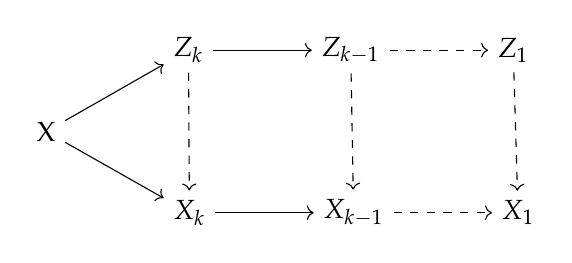
\begin{tikzpicture}
   %Nodes
  \node (X) {X};
  \node[above right=0.5cm and 1.25cm of X] (Y) {$Z_k$};
  \node[below right=0.5cm and 1.25cm of X] (Z) {$X_k$};
  \node[right=1.25cm of Y] (A) {$Z_{k-1}$}; 
  \node[right=1.25cm of Z] (B) {$X_{k-1}$};
  \node[right=1.25cm of A] (C) {$Z_1$};
  \node[right=1.25cm of B] (D) {$X_1$};

  %Arrows
  \draw[->] (X) -- (Y);
  \draw[->] (X) -- (Z);
  \draw[->, dashed] (Y) -- (Z);
  \draw[->] (Y) -- (A);
  \draw[->] (Z) -- (B);
  \draw[->, dashed] (A) -- (B);
  \draw[->, dashed] (A) -- (C);
  \draw[->, dashed] (B) -- (D);
  \draw[->, dashed] (C) -- (D);
\end{tikzpicture}
\end{center}
 where \( Z_i \dasharrow X_i \) indicates either a measurable isomorphism for all $i$ or a proper factor map for each $i$. We construct examples realizing all possible behaviors in between these two phenomena. Understanding when the measurable and topological nilfactors are different constitutes partly to the goal of this paper. We note in a weak mixing system all nilfactors are trivial (see, for example, Proposition 20 of Chapter 8 in \cite{HK2}). We also note that nilsystems are classic examples of systems with $Z_k$ and $X_k$ isomorphic. 

    
%Let $(X,\mu,T)$ be a minimal and ergodic system, meaning $X$ is a compact metric space, $T$ is a minimal homeomorphism of $X$, and $\mu$ is a $T$-invariant ergodic Borel probability measure. 
%The measurable $k$-step nilfactor of $X$ has been shown in works of Host and Kra in \cite{HK paper} to control the dynamical behavior of certain multiple ergodic averages. More recently, these factors have appeared in \cite{a model with topological pronilfactors} where Kra, Moreira, Richter and Robertson, solved a conjecture of Erd\H{o}s on sumsets. There, it was shown how these nilfactors control certain infinite patterns in sets with positive density. The topological analog of these factors was first introduced by Host, Kra and Maass in \cite{Host Kra and Maass}. In many examples of systems, either the measurable and topological $k$-step nilfactors, $Z_k$ and $X_k$, are measurably isomorphic for all $k$, or they are not for each $k$, with the latter slightly harder to construct. Every ergodic system is measurably isomorphic to a strictly ergodic system whose $Z_i$ and $X_i$ factors are measurably isomorphic for all $i\in \mathbb{N}$ (see, for example, \cite{maximal pronilfactors}). On the other hand, by a theorem of Lehrer \cite{Lehrer}, it follows that every ergodic, non-weak mixing system is measurably isomorphic to a strictly ergodic system where $Z_1$ and $X_1$ are not measurably isomorphic, hence $Z_i$ and $X_i$ are not isomorphic as well. % The examples with nonisomorphic measurable and topological $k$-step nilfactors tend to be built from a system where we already have $Z_1$ not measurably isomorphic to $X_1$. 
% These examples can be found in, for instance, \cite{{nontrivial Kronecker trivial MEF}, {Gla}, {Lehrer}, {Parry}}. 

 %For $k\geq 2$, The examples with nonisomorphic measurable and topological $k$-step nilfactors tend to be built from a system where we already have $Z_1$ not measurably isomorphic to $X_1$. 
%In fact, in many systems, either $Z_k$ is measurably isomorphic to $X_k$ for all $k$ or $Z_k$ is not measurably isomorphic to $X_k$ for each $k$. We illustrate this phenomenon in the diagram below %Our goal in this paper is to construct examples which realize all possible behaviors in between, capturing the flexibility of these nilfactors. 

 \begin{theorem}\label{the theorem in introduction}
For all $0 \leq j \leq \ell \leq k,\; k\geq 1$, there exists a strictly ergodic system which admits the following:
\begin{enumerate}
    \item $Z_k$ is a nontrivial extension of $Z_{k-1}$
    \item $Z_i$ is topologically isomorphic to $X_i$ for all $0 \leq i \leq j$
    \item $Z_i$ is not measurably isomorphic to $X_i$ for all $j+1 \leq i \leq k$
    \item $X_i$ is topologically isomorphic to $X_{i+1}$ for all $i \geq \ell$.

\end{enumerate}
Furthermore, for every minimal, ergodic, and non-weak mixing $(X,\mu,T)$ there exist $j,\ell$, and $k$, such that $X$ satisfies properties (1)-(4).
 \end{theorem}

To prove Theorem \ref{the theorem in introduction}, we draw inspiration from an example of a minimal but not uniquely ergodic system constructed by Furstenberg in \cite{Fur61}. There, it is shown that for $\alpha \notin \mathbb{Q}$, the system $$T(x,y)=(x+\alpha,y+f(x)), \;\;T\colon\mathbb{T}^{2} \rightarrow \mathbb{T}^{2}$$ is minimal and not uniquely ergodic if and only if 
\begin{equation}\label{eq: coboundary furstenberg}
nf \equiv F(x+\alpha)-F(x) \mod 1
\end{equation}
has a measurable solution for some $n \in \mathbb{Z} \setminus \{0\}$ but no continuous solution unless $n=0$. In \cite{Fur61}, an $f$ which has a measurable solution for $n=1$ but no continuous solution except when $n=0$ is constructed. We refer to $f$ as a measurable but not continuous coboundary over the system $(\mathbb{T},m_{\mathbb{T}},T_{\alpha})$. In Section \ref{sec: flexibility}, we use these coboundaries to construct systems where the measurable and topological $k$-step nilfactors are not measurably isomorphic after some point.

In Proposition \ref{nontrivial measurable nils but trivial topological nils}, we exhibit another flexibility of the nilfactors where for each $k\in \mathbb{N}$, we build a strictly ergodic system which has $Z_k$ as a nontrivial extension of $Z_{k-1}$ yet has trivial topological nilfactors. Such examples are known to exist by Lehrer \cite{Lehrer}, however, we provide a construction that is more explicit using a certain minimal Cantor system built by Durand, Frank, and Maass, in \cite{nontrivial Kronecker trivial MEF} along with techniques we develop in this article from Proposition \ref{proposition with one coboundary on k}.
 
 %We explore examples of systems where we have both behaviors, constituting partly to the goal of this paper.


%We show the complete flexibility of the measurable and topological nilfactors among systems and we make this precise in our main result below (see Section \ref{sec: notations and preliminaries} for definitions and notations).

 %\begin{theorem}\label{the theorem in introduction}
%For all $0 \leq j \leq \ell \leq k,\; k\geq 1$ there exists a strictly ergodic system which admits the following:
%\begin{enumerate}
 %   \item $Z_k$ is a nontrivial extension of $Z_{k-1}$
 %   \item $Z_i$ is topologically isomorphic to $X_i$ for all $0 \leq i \leq j$
  %  \item $Z_i$ is not measurably isomorphic to $X_i$ for all $j+1 \leq i \leq k$
  %  \item $X_i$ is topologically isomorphic to $X_{i+1}$ for all $i \geq \ell$.

%\end{enumerate}
%Furthermore, subject to the standard constraints, the above properties capture all possible behaviors of a minimal, ergodic, non-weak mixing dynamical system.
 %\end{theorem}

 
 
 
 
 %Given an ergodic system $(X,\mu,T)$, $Z_k$ being isomorphic to $X_k$ is equivalent to the existence of a continuous factor map from $X \rightarrow Z_k$ (see Lemma \ref{Zk and Xk measurably iso iff cont factor map} in Section \ref{Host-Kra structure theory}). In \cite{a model with topological pronilfactors} a continuous factor map to $Z_1$ was needed. 



 % For the case when $k=1$, it is mentioned in \cite{Parry} that for $\alpha,\beta \notin \mathbb{Q}$ rationally independent and for a measurable but not continuous coboundary $f:\mathbb{T} \rightarrow \mathbb{T}$ over $(\mathbb{T},m_{\mathbb{T}},T_{\alpha})$, the system $(\mathbb{T}^{2},m_{\mathbb{T}^{2}},T)$ where $$T(x,y)=(x+\alpha,y+f(x)+\beta),\; T:\mathbb{T}^{2} \rightarrow \mathbb{T}^{2},$$ $Z_1$ is given by $(x,y)\mapsto (x+\alpha,y+\beta)$ and $X_1$ is given by just $x\mapsto x+\alpha$. Writing $f=F\circ T_{\alpha}-F$, the latter is easily seen by noticing the eigenfunctions for $T$ are $f_{n,m}(x,y)=e(nx)e(my-mF(x))$ which are continuous only when $m=0$. We also note in \cite{Gla} the same example was studied but using instead the regionally proximal relation to compute $X_1$.

 

    %\begin{definition}
    %An admissible diagram is any graph of the form 
    \begin{comment}
   \begin{center}
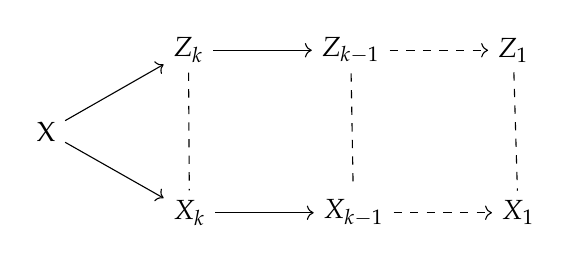
\begin{tikzpicture}
   %Nodes
  \node (X) {X};
  \node[above right=0.5cm and 1.25cm of X] (Y) {$Z_k$};
  \node[below right=0.5cm and 1.25cm of X] (Z) {$X_k$};
  \node[right=1.25cm of Y] (A) {$Z_{k-1}$}; 
  \node[right=1.25cm of Z] (B) {$X_{k-1}$};
  \node[right=1.25cm of A] (C) {$Z_1$};
  \node[right=1.25cm of B] (D) {$X_1$};

  %Arrows
  \draw[->] (X) -- (Y);
  \draw[->] (X) -- (Z);
  \draw[dashed] (Y) -- (Z);
  \draw[->] (Y) -- (A);
  \draw[->] (Z) -- (B);
  \draw[dashed] (A) -- (B);
  \draw[->, dashed] (A) -- (C);
  \draw[->, dashed] (B) -- (D);
  \draw[dashed] (C) -- (D);
\end{tikzpicture}
\end{center}
\end{comment}
\begin{comment}
\hfill
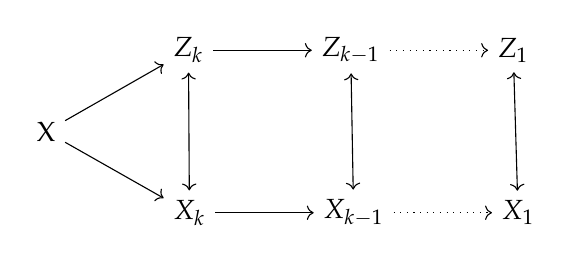
\begin{tikzpicture}
   %Nodes
  \node (X) {X};
  \node[above right=0.5cm and 1.25cm of X] (Y) {$Z_k$};
  \node[below right=0.5cm and 1.25cm of X] (Z) {$X_k$};
  \node[right=1.25cm of Y] (A) {$Z_{k-1}$}; 
  \node[right=1.25cm of Z] (B) {$X_{k-1}$};
  \node[right=1.25cm of A] (C) {$Z_1$};
  \node[right=1.25cm of B] (D) {$X_1$};

  %Arrows
  \draw[->] (X) -- (Y);
  \draw[->] (X) -- (Z);
  \draw[<->] (Y) -- (Z);
  \draw[->] (Y) -- (A);
  \draw[->] (Z) -- (B);
  \draw[<->] (A) -- (B);
  \draw[->, dotted] (A) -- (C);
  \draw[->, dotted] (B) -- (D);
  \draw[<->] (C) -- (D);
\end{tikzpicture}

\end{comment}
\begin{comment}
An interesting corollary of Theorem \ref{the theorem in introduction} is that there exists a strictly ergodic system whose behavior is described in the diagram below.
\begin{center}
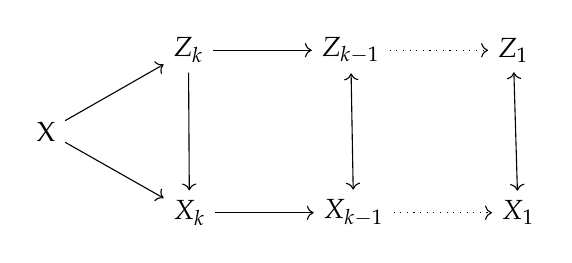
\begin{tikzpicture}
   %Nodes
  \node (X) {X};
  \node[above right=0.5cm and 1.25cm of X] (Y) {$Z_k$};
  \node[below right=0.5cm and 1.25cm of X] (Z) {$X_k$};
  \node[right=1.25cm of Y] (A) {$Z_{k-1}$}; 
  \node[right=1.25cm of Z] (B) {$X_{k-1}$};
  \node[right=1.25cm of A] (C) {$Z_1$};
  \node[right=1.25cm of B] (D) {$X_1$};

  %Arrows
  \draw[->] (X) -- (Y);
  \draw[->] (X) -- (Z);
  \draw[->] (Y) -- (Z);
  \draw[->] (Y) -- (A);
  \draw[->] (Z) -- (B);
  \draw[<->] (A) -- (B);
  \draw[->, dotted] (A) -- (C);
  \draw[->, dotted] (B) -- (D);
  \draw[<->] (C) -- (D);
\end{tikzpicture}
\end{center}

\end{comment}

%Systems which have a continuous factor map to their $k$-step pronilfactors are also studied by Gutman and Lian in \cite{maximal pronilfactors}. %Although we do not inherit this terminology in the paper, a corollary of Theorem \ref{the theorem in introduction} would then be that for all $k\in \mathbb{N}$ there exists a strictly ergodic system which is CF-Nil($k-1$) but not CF-Nil($k$). 


%For an ergodic system $(X, \mu, T)$, the measurable $k$-step nilfactor of $X$, denoted by $(Z_{k},m_{Z_k},T)$, is the maximal measurable factor that is an inverse limit of measurable $k$-step nilsystems. Here, \textit{maximal} means every measurable factor which is an inverse limit of $k$-step nilsystems is a measurable factor of $Z_{k}$. It comes with an associated \textit{measurable} factor map $\pi_{k}:X \rightarrow Z_k$. Similarly, if we have a minimal system $(X,T)$, then the topological $k$-step nilfactor of $X$, denoted by $(X_{k}, T)$, is the maximal topological factor that is an inverse limit of $k$-step topological nilsystems, where \textit{maximal} is now with respect to topological factors. It also has an associated \textit{topological} factor map $\rho_{k}:X \rightarrow X_k$. 
%Furstenberg constructed an example of a minimal but not uniquely ergodic analytic diffeomorphism on $\mathbb{T}^2$. Since then, his example has been widely used to build systems which have different measurable and topological properties. For self-containment purposes, we will highlight the details of Furstenberg's construction since it will be used later for the examples with non-measurably isomorphic measurable and topological Host-Kra factors of order $k$. The following lemma of Furstenberg's is the heart of how to construct a minimal but not uniquely ergodic system.

% \begin{lemma}[Furstenberg 1961]
  %  Let $\alpha \notin \mathbb{Q}$, $f:\mathbb{T} \rightarrow \mathbb{T}$ be continuous, and let $T: \mathbb{T}^{2} \rightarrow \mathbb{T}^{2}$ be defined by $$T(x,y)=(x+\alpha,y+f(x)).$$ Then $T$ is minimal if and only if there does not exist a continuous solution $F:\mathbb{T}\rightarrow \mathbb{T}$ to the following equation: $$f(x) = F(x+\alpha)-F(x). \;\;\;\; (1)$$ Furthermore, $T$ is uniquely ergodic if and only if the latter equation does not admit a measurable solution $F$.
%\end{lemma}




\section{Preliminaries}
\label{sec: notations and preliminaries}

\subsection{Definitions and notations}\label{definition}
Throughout $\mathbb{N}$ denotes the set $\{1,2, 3, \dots \}$. By a dynamical system we mean any triple of the form $(X, \mu, T)$ where $X$ is a compact metric space endowed with the Borel $\sigma$-algebra and $T$ is a homeomorphism of $X$ preserving a Borel probability measure $\mu$. Namely, for any Borel set $B \subseteq X$ we have $\mu(T^{-1}(B))=\mu(B).$ Given two compact metric spaces $X$, $Y$, and a measurable map $f\colon X \rightarrow Y$, the push forward of $\mu$ under $f$ is the invariant measure on $Y$ defined by $(f_{*}\mu)(B)=\mu(f^{-1}(B))$ for all $B \subseteq Y$.



Since we have assumed throughout that the setting of our dynamical systems has an underlying topological structure, this allows us to discuss both measurable and topological factors.




    For a system $(X,\mu,T)$, we say $(Y,\nu,S)$ is a \textit{measurable factor} of $(X,\mu,T)$ if there exists a measurable map $\pi\colon X \rightarrow Y$, \textit{the measurable factor map}, such that $(S \circ \pi)(x)= (\pi \circ T)(x)$ for $\mu$-almost every $x \in X$ and $\pi_{*} \mu=\nu.$ Furthermore, if $\pi$ is a bijection with $\pi^{-1}$ measurable, then it is a \textit{measurable isomorphism}. We say $(Y, \nu, S)$ is a \textit{topological factor} of $(X, \mu, T)$ if there exists a continuous and surjective map $\rho\colon X \rightarrow Y$, \textit{the topological factor map}, such that $(S \circ \rho)(x)= (\rho \circ T)(x)$ for all $x\in X$ and $\rho_{*}  \mu=\nu.$ If $\rho\colon X \rightarrow Y$ is a homeomorphism, then it is a \textit{topological isomorphism}. We use the notation $\overset{m}\cong$ and $\overset{t}\cong$ to denote measurable and topological isomorphisms, respectively. 

%We will use the notations $\overset{m}\longleftrightarrow$ and $\overset{t}\longleftrightarrow$ to denote measurable and topological isomorphisms, respectively. Similarly, $\overset{m}\longrightarrow$ and $\overset{t}\longrightarrow$ will denote nontrivial measurable and topological extensions respectively. 

%Sometimes if $\pi:X \rightarrow Y$ is a factor map (measurable or topological), then we will say $X$ is an extension of $Y$. We will also differentiate between measurable and topological isomorphisms so we provide those definitions below.

%\begin{definition}
   % A system $(X,\mu,T)$ is measurably isomorphic to a system $(Y,\nu,S)$ if there exists a measurable factor map $\pi:X \rightarrow Y$, a $T$-invariant set $A \in \mathcal{X}$ with $\mu(A)=1$, and a $S$-invariant set $B \in \mathcal{Y}$ with $\nu(B)=1$ such that $\pi$ restricted onto $A$ is a bijection into $B$.
%\end{definition}

%\begin{definition}
   %  A system $(X,\mu,T)$ is topologically isomorphic to a system $(Y,\nu,S)$ if there exists a bijective topological factor map $\rho:X \rightarrow Y$.
%\end{definition}




%By $ \longleftrightarrow $, we will always be indicating a measurable isomorphism. If we have $\updownarrow$ between topological factors, then we will be indicating a topological isomorphism and similarly between measurable factors it will denote a measurable isomorphism. The symbol $\longrightarrow $ between two measurable objects will apriori denote a measurable factor map (or nontrivial extension) and it will be a topological factor map between two topological objects. 



%The objects useful in the discussion here are nilsystems which are translations on nilmanifolds. 
Given a $k$-step nilpotent Lie group $G$ and $\Gamma \leq G$ a discrete cocompact subgroup, $X=G/\Gamma$ is a \textit{$k$-step nilmanifold}. Now fix $g \in G$. Then $T\colon X \rightarrow X$ given by $x \mapsto  g \cdot x$ is a \textit{nilrotation.} The Haar measure on $X$ is the unique measure invariant under all nilrotations and we denote it by $m_X$. A system $(X,m_X,T)$ where $X$ is a $k$-step nilmanifold and $T$ is a nilrotation is a \textit{$k$-step nilsystem}. A special class of nilsystems we consider are \textit{affine nilsystems}. Let $A$ be a $k\times k$ unipotent integer matrix, $b\in \mathbb{T}^{k}$, and $T\colon \mathbb{T}^{k} \rightarrow \mathbb{T}^{k}$ be given by $x \mapsto Ax+b$. Then $(\mathbb{T}^{k},m_{\mathbb{T}^{k}},T)$ is a \textit{$k$-step affine nilsystem}. Note there are nilsystems which are not affine.


%This allows us to naturally associate any topological $k$-step nilsystem to a measurable one, namely $(X,m_{X},T)$.



We say $(Y,\nu,S)$ is a \textit{maximal factor of $(X,\mu,T)$ with property $\mathcal{P}$} if every factor of $X$ with Property $\mathcal{P}$ is a factor of $Y$. For an ergodic system $(X, \mu, T)$, \textit{the measurable $k$-step nilfactor of $X$}, denoted by $Z_{k}$, is the maximal measurable factor that is an inverse limit of $k$-step nilsystems, \textit{maximal} being with respect to measurable factor maps. %means every $k$-step nilsystem that is a measurable factor of $X$ is a measurable factor of $Z_{k}$. %Its associated \textit{measurable} factor map we denote by $\pi_{k}\colon X \rightarrow Z_k$.
Similarly, if we have a minimal system $(X,T)$, then \textit{the topological $k$-step nilfactor of $X$}, denoted by $X_{k}$, is the maximal topological factor that is an inverse limit of $k$-step nilsystems, where \textit{maximal} is now with respect to topological factors. %When there is room for ambiguity, we write $Z_k(T)$ or $X_k(T)$ to specify the transformation. 
Uniqueness (up to isomorphism) for the maximal measurable nilfactors is easily seen via the semi-norm presentation given in \cite{HK paper}, and for the topological nilfactors, via the regionally proximal relation of order $k$ in \cite{Host Kra and Maass}. %We denote the associated \textit{topological} factor map by $\rho_{k}\colon X \rightarrow X_k$. 
The factors $Z_0$ and $X_0$ are both the trivial one-point system. 
%In particular, the spaces associated to these factors do not need to be nilmanifolds; but we always have a topology inherited from the inverse limit structure. 
%For inverse limits of nilsystems, minimality is equivalent to unique ergodicity (with the unique measure being Haar). This allows us to view $(X_k,T)$ as a measurable factor $(X_k,m_{X_k},T)$. %A system is strictly ergodic if it is both minimal and uniquely ergodic.
%Sometimes when two systems $(X,\mu,T)$ and $(Y,\nu,S)$ are in discussion, we will write $Z_{k}(X)$ to denote the $k$-step nilfactor of $X$ and $Z_{k}(Y)$ to denote the $k$-step nilfactor of $Y$. 



The factor $X_k$ is naturally endowed with Haar measure because for inverse limits of nilsystems, minimality is equivalent to unique ergodicity, the unique measure being Haar (see \cite{HK2}). In this way, we can view $X_k$ not only as a topological factor of our system but also as a measurable factor. Systems that are both minimal and uniquely ergodic are \textit{strictly ergodic}. 

Since $Z_k$ is the \textit{maximal} measurable $k$-step nilfactor, there exists a measurable factor map which we denote by $\tau_{k}\colon Z_k \rightarrow X_k$, $k\in \mathbb{N}$. Also, since $Z_k$ is in particular an inverse limit of $(k+1)$-step nilsystems, by maximality of $Z_{k+1}$, we have a measurable factor map $ Z_{k+1}\rightarrow Z_k$ and similarly we have a topological factor map $ X_{k+1} \rightarrow X_k$ for all $k\in \mathbb{N}$. 



%The following fact is very obvious. We use it when it is more convenient to describe the measurable nilfactors of a system that is measurably isomorphic to the system we have. The topological analog is also true.

%\begin{fact} \label{isomorphic systems have isomorphic nils}
  %  Measurably (topologically) isomorphic systems have isomorphic measurable (topological) $k$-step nilfactors.
%\end{fact}




\subsection{Necessary constraints} \label{standard constraints} There are necessary constraints to the behavior of nilfactors within a system. We summarize them below:
  \begin{enumerate}

    \item If $Z_i\overset{m}\cong Z_{i+1}$ for some $i\geq 0$, then $Z_j\overset{m}\cong Z_i$ and $X_j\overset{t}\cong X_i$ for all $j \geq i$ (follows from combining Theorem 12 in Chapter 16 of \cite{HK2} and Proposition 4.11 and Theorem 10.1 of \cite{HK paper})
    
    %The first implication of measurable nilfactors coinciding follows from Theorem 12 in Chapter 16 of \cite{HK2} and $X_j\overset{t}\cong X_i$ follows by combining Proposition 4.11 and Theorem 10.1 of \cite{HK paper}).
    
     %\noindent The first implication of $Z_j\overset{m}\cong Z_i$ is Theorem 12 in Chapter 16 of \cite{HK2} and the second implication of $X_j\overset{t}\cong X_i$ follows by Theorem 5 in Chapter 13 of \cite{HK2}.
     
    \item If $X_i\overset{t}\cong X_{i+1}$ for some $i \geq 0$, then $X_j\overset{t}\cong X_i$ for all $j \geq i$ (see Theorem 3.8 of \cite{Dong}).
    
     \item If $Z_i\overset{m}\cong X_i$ for some $i \geq 0$, then $Z_j\overset{m}\cong X_j$ for all $j \leq i$ (since a measurable isomorphism between two systems induces bijections between their factors).

     
  %   \item If $Z_1$ or $X_1$ is trivial, then for all $i \geq 1$, $Z_i$ or $X_i$ is trivial, respectively. (a trivial $Z_1$ factor implies 
     
     %(A trivial $Z_1$ factor is equivalent to a system being measurably weak mixing (see Theorem 1.26 in \cite{Walters}). Weak mixing systems have trivial nilfactors (see Proposition 20, Chapter 8 of\cite{HK2}). Analogously, a trivial $X_1$ factor is equivalent to a system being topologically weak mixing, which is further equivalent to trivial topological nilfactors (see Theorem 3.13 in \cite{Shao and Ye}).)
\end{enumerate}

\subsection{Intermediate factors} 

Let $(Y,\nu,T)$ be a system and $K$ be a compact abelian group. The system $(Y\times K,\nu \times m_K, T)$, defined by $T(y,k)=(Ty,\rho(y)+k)$ with $\rho\colon Y \rightarrow K$ measurable, is an \textit{extension of $Y$ by $K$}. For $h \in K$, the map $V_h\colon Y \times K \rightarrow Y \times K$ given by $V_h(y,k)=(y,k+h)$ is a \textit{vertical rotation}. 

The following can be deduced from the proof of Lemma 7.3 in \cite{Furstenberg and Weiss}. We use the more detailed description in \cite{HK2}.
   % \begin{lemma}[Furstenberg and Weiss \cite{Furstenberg and Weiss}]\label{intermediate extensions}

%Let $X=Y \times K$ be an ergodic group extension of $Y$ and $W$ is an intermediate extension of $Y$, then $W$ is a group extension of $Y$ by the group $K/H$, where $H\leq G$ is a closed subgroup. 

\begin{lemma}[Host and Kra, Chapter 5, Lemma 19 \cite{HK2}] \label{intermediate extensions}
   Let $\pi\colon (X,\mu,T) \rightarrow (Y,\nu,S)$ be an extension by a compact abelian group $K$ such that $(X,\mu,T)$ is ergodic and let $p\colon W \rightarrow Y$ be an intermediate extension, meaning there exists a factor map $q\colon X \rightarrow W$ such that $p\circ q=\pi.$ Then $W$ is the quotient of $X$ under the action of some closed subgroup $H \leq K$, acting by vertical rotations.
\end{lemma}



\subsection{Coboundaries}
\begin{definition}\label{def of cob}
    For a system $(Y,\nu,T)$ and a compact abelian group $K$, we say $\rho\colon Y \rightarrow K$ is a \textbf{coboundary over $(Y,\nu,T)$} if there exists $ F\colon Y \rightarrow K$ measurable such that 
    \begin{equation} \label{eq:coboundary}
        \rho=F \circ T - F.
    \end{equation}
\end{definition}











\begin{remark} \label{cob soln are unique}
    Given an ergodic system $(X,\mu,T)$ and a coboundary $\rho\colon X \rightarrow \mathbb{T}$ over $(X,\mu,T)$, the solutions to the cohomological equation \eqref{eq:coboundary} are unique up to a constant. Indeed, suppose $\rho=f\circ T - f=g\circ T- g$ for some $f,g\colon  X \rightarrow \mathbb{T}$. We immediately have $f - g$ is $T$-invariant, hence constant by ergodicity.
\end{remark}


We refer to $\rho$ as a \textit{measurable but not continuous coboundary} if we have a measurable solution $F\colon Y \rightarrow K$ in \eqref{eq:coboundary} and there exists no continuous solution. However, $\rho$ itself is continuous throughout.







%We also note that a system being measurably weak mixing is equivalent to having a trivial $Z_1$, and similarly, a system being topologically weak mixing is equivalent to having a trivial $X_1$.

%The first part of fact 1 is in Host and Kra (see Theorem 12, Chapter 16 of \cite{HK2}). The second part about the topological nilfactors follows immediately by the universal property of $X_i$. Fact 2 is a result of Dong, Donoso, Maass, Shao and Ye (see Theorem 3.8 of \cite{Dong}). Fact 3 is by Gutman and Lian (see Theorem 2.32 in \cite{maximal pronilfactors}). Having a trivial $Z_1$ factor is equivalent to a system being measurably weak mixing, and this is a classical fact which can be found in \cite{Walters}. This also implies all higher order measurable nilfactors are trivial (see Proposition 20, Chapter 8 of\cite{HK2}). Analogously, having a trivial $X_1$ factor is equivalent to a system being topologically weak mixing, which is further equivalent to trivial higher order topological nilfactors (see Theorem 3.13 in \cite{Shao and Ye}).






%\end{center}
%which obeys the following facts
%\begin{enumerate}
    %\item If $Z_i=Z_{i+1}$ for some $i$, then $Z_j=Z_i$ for all $j \geq i$.
    %\item If $X_i=X_{i+1}$ for some $i$, then $X_j=X_i$ for all $j \geq i$.
    %\item If $Z_i=X_i$ for some $i$, then $Z_j=X_j$ for all $j \leq i$.
%\end{enumerate}




%\end{definition}

%\begin{theorem}
   % For every ergodic system $(X,\mu,T)$ and admissible diagram, there exists a strictly ergodic system $(Y,\nu,S)$ measurably isomorphic to $(X,\mu,T)$ having the same diagram.
%\end{theorem}

%\begin{corollary}
    %For any admissible diagram, there exists a system realizing it. 
%\end{corollary}



%Sometimes when two systems $(X,\mu,T)$ and $(Y,\nu,S)$ are in discussion, we will write $Z_{k}(X)$ (or $X_{k}(X)$ to denote the $k$-step nilfactor of $X$ and $Z_{k}(Y)$ to denote the $k$-step nilfactor of $Y$. 

\subsection{Eigenfunctions}\label{eigenfunctions}

Given a system $(X,\mu,T)$, we say $f\colon X \rightarrow \mathbb{S}^{1}$, is an \textit{eigenfunction} if there exists $ \lambda \in \mathbb{S}^{1}$ such that $f\circ T=\lambda f$. It is a classical fact that a system having a trivial $Z_1$ (resp. $X_1$) is equivalent to being measurably (resp. topologically) weak mixing which is further equivalent to the system having no non-constant measurable (resp. continuous) eigenfunctions (see, for example, \cite{Shao and Ye} and \cite{Walters}). Furthermore, $L^2(Z_1)$ and $C(X_1)$ are spanned by the measurable and continuous eigenfunctions of $X$, respectively. In \cite{Parry}, it is mentioned for $\alpha,\beta \notin \mathbb{Q}$ rationally independent, and for a measurable but not continuous coboundary $f\colon \mathbb{T} \rightarrow \mathbb{T}$ over $(\mathbb{T},m_{\mathbb{T}},T_{\alpha})$, for the system $(\mathbb{T}^{2},m_{\mathbb{T}^{2}},T)$ where $$T(x,y)=(x+\alpha,y+f(x)+\beta),\; T\colon \mathbb{T}^{2} \rightarrow \mathbb{T}^{2},$$ $Z_1$ is $(\mathbb{T}^{2},m_{\mathbb{T}^{2}},T_{\alpha,\beta})$ and $X_1$ is $(\mathbb{T},T_{\alpha})$. Writing $f=F\circ T_{\alpha}-F$, the latter is easily seen by noticing the eigenfunctions for $T$ are $f_{n,m}(x,y)=e(nx)e(my-mF(x))$, $(n,m)\in \mathbb{Z}^{2}$, which are continuous only when $m=0$. We also note in \cite{Gla} the same example was studied but instead using the regionally proximal relation to compute $X_1$.

%\subsection{Strong orbit equivalence}\label{strong orbit equivalence}

%Given two systems $(Y,S)$, $(Z,T)$, and the homeomorphism $h\colon Y \rightarrow Z$ is a \textit{strong orbit equivalence} if $(T\circ h)(y)=(h \circ S^{j(y)})(y)$ and $(h \circ S)(y)=(T^{m(y)} \circ h)(y)$ for some $j,m\colon Y \rightarrow \mathbb{Z}$ with each having at most one point of discontinuity. Let $\alpha \notin \mathbb{Q}$ and $(X_\alpha,\sigma)$ denote the Sturmian subshift. By Corollary 23 of \cite{nontrivial Kronecker trivial MEF}, there exists a minimal topologically weak mixing system $(X,T)$ which is strong orbit equivalent to $(X_{\alpha},\sigma)$. It follows from Theorem 2.2 in \cite{Giordano}, that if $(Y,S)$ is uniquely ergodic and orbit equivalent to $(Y',S')$ (in particular, strong orbit equivalent), then $(Y',S')$ is uniquely ergodic. Hence, $(X,T)$ is uniquely ergodic. We use this example in Proposition \ref{nontrivial measurable nils but trivial topological nils}.


\begin{comment}
\section{Intermediate lemmas} \label{Host-Kra structure theory}
\end{comment}

%    For a system $(Y,\nu,T)$ and $K$ a compact abelian group, a measurable map $\rho\colon Y \rightarrow K$ is a \textit{cocycle}. 
    %If $\rho \colon Y \rightarrow K$ is a cocycle, then the \textit{extension} (of $Y$ by $K$) \textit{defined by $\rho$} is the extension $\pi\colon (Y \times K, \nu \times m_{K}, T_{\rho}) \rightarrow (Y,\nu,T)$, where $\pi\colon Y \times K \rightarrow Y$
%is the projection $(y,k) \mapsto y$ and $$T_{\rho}(y,k)=(Ty,\rho(y)+k) \;\;\; \mathrm{for}\; (y,k) \in Y \times K.$$


%A cocycle $\rho$ is \textit{ergodic} if the extension defined by $\rho$ gives rise to an ergodic system. A system is \textit{strictly ergodic} if it is both minimal and uniquely ergodic.

%\begin{definition}\label{def of cob}
   % For a system $(Y,\nu,T)$ and $K$ a compact abelian group, we say $\rho\colon Y \rightarrow K$ is a \textbf{coboundary over $(Y,\nu,T)$} if there exists $ F\colon Y \rightarrow K$ measurable such that 
   % \begin{equation} \label{eq:coboundary}
   %     \rho=F \circ T - F.
   % \end{equation}
%\end{definition}











%\begin{remark} \label{cob soln are unique}
   % Given an ergodic system $(X,\mu,T)$ and a coboundary $\rho\colon X \rightarrow \mathbb{T}$ over $(X,\mu,T)$, the solutions of $\rho$ to the cohomological equation in \eqref{eq:coboundary} are unique up to a constant. Indeed, suppose $\rho=f\circ T - f=g\circ T- g$ for some $f,g\colon  X \rightarrow \mathbb{T}$. We immediately have $f - g$ is $T$-invariant, hence constant by ergodicity.
%\end{remark}





%\begin{definition}
    % For a system $(Y,\nu,T)$ and $K$ a compact abelian group, we say $\rho\in \mathrm{Coc}(Y,K)$ is a \textbf{cocycle of type $1$} if  $\exists F: Y \times Y \rightarrow K$ measurable such that
% $$\rho(y_0)-\rho(y_1)=F(Ty_0,Ty_1)-F(y_0,y_1)$$ for $\nu \times \nu$ almost every $(y_0,y_1)$.
%\end{definition}

%For $\rho \in \mathrm{Coc}(Y,K)$, we have the cocycle $\Delta \rho$ on $Y^{[1]}=Y \times Y$ given by $\Delta \rho (y_0,y_1):=\rho(y_0)-\rho(y_1)$ and for $k \geq 2$ we can inductively define $$\Delta^{[k]}\rho(\textbf{y})= \sum_{\underline{\epsilon} \in [k]} (-1)^{|\underline{\epsilon}|} \rho(y_{\underline{\epsilon}}) \;\;\; \mathrm{for} \;\; \textbf{y} \in Y^{[k]}, \mathrm{where}\; Y^{[k]} \; \mathrm{is \; a \; product\; of\; 2^k \; copies \; of \; Y}.$$

%\begin{definition}
   % For a system $(Y,\nu,T)$ and $K$ a compact abelian group, we say $\rho\in \mathrm{Coc}(Y,K)$ is a \textbf{cocycle of type $k$} if $\Delta ^{[k]} \rho: Y^{[k]} \rightarrow K$ is a coboundary of the system $(Y^{[k]},\nu^{[k]},T^{[k]})$. i.e. $\exists F: Y^{[k]} \rightarrow K$ measurable such that 
   % \begin{equation} \label{eq:cocycle of type k}
    %\Delta ^{[k]} \rho = F \circ T^{[k]}-F .
    %\end{equation}
%\end{definition}

%We will refer to $\rho$ as a \textit{measurable but not continuous cocycle of type $k$} if we have a measurable solution $F$ in \eqref{eq:cocycle of type k} and that there does not exist any continuous solution. Our cocycles themselves will always be continuous throughout.

%We refer to $\rho$ as a \textit{measurable but not continuous coboundary} if we have a measurable solution $F\colon Y \rightarrow K$ in \eqref{eq:coboundary} and there exists no continuous solution. Our cocycles themselves are always continuous throughout.

\begin{comment}

Two cocycles $\phi,\phi':Y \rightarrow K$ are \textit{cohomologous} if $\phi -\phi'$ is a coboundary over $(Y,\nu,T)$. We denote it by $\phi \sim \phi'$. It is well known that the extensions defined by cohomologous cocycles over the same system give rise to isomorphic systems. Since we frequently use this fact throughout the proof, we provide it below for completeness.

\smallskip

\begin{lemma}\label{cohomologous cocycles give isomorphic systems}
    For $\phi, \phi': Y \rightarrow K$ with $\phi \sim \phi'$, the extensions defined by $\phi$ and $\phi'$ over $(Y,\nu,S)$ are isomorphic.
\end{lemma}

\begin{proof}
    Since $\phi \sim \phi'$ we have $\phi-\phi' = F \circ T -F$ for some $F: Y \rightarrow K$. Then the extensions defined by each of the cocycles $T_{\phi}$ and $T_{\phi'}$ are isomorphic via the map $\pi:Y \times K \rightarrow Y \times K$ given by $\pi(y,k)=(y,k-F(y))$. Indeed, $$\pi \circ T_\phi (y,k)= (Ty, k+\phi(y)-F(Ty))=(Ty,k-F(y)+\phi'(Ty))=T_{\phi'} \circ \pi(y,k).$$ \end{proof}
    
   % We illustrate this in the commutative diagram below: 
    %\[
%\begin{tikzcd}
  %(Y \times K,\nu \times m_K) \arrow[r, "T_{\phi}"] \arrow[d, "\pi"'] & 
  %(Y \times K,\nu \times m_K)
 %  \arrow[d, "\pi"] \\
  %(Y \times K,\nu \times m_K)
  %\arrow[r, "T_{\phi'}"'] & 
 % (Y \times K,\nu \times m_K)
%\end{tikzcd}
%\] 

\end{comment}


%Although the notation $\mathrm{Coc}_{k}(Y,K)$ denotes all of the measurable maps from $Y \rightarrow K$, for our setting the cocycles will always be continuous maps, unless otherwise specified.

%\begin{lemma} [Host-Kra]\label{cocycles of type k are a group}
    %Given a system $(Y,\nu,T)$ and $K$ a compact abelian group, the set of all continuous $K$-valued cocycles of type $k$, denoted by $C_{k}(Y,K)$, form an additive group. 
%\end{lemma}

%\begin{theorem}[Host-Kra] \label{thm:Z_k}
   % Given $k \in \mathbb{N}$ and an ergodic system $(X,\mu,T)$, we say $X$ is of order $k$ if and only if it is an inverse limit (in the measure-theoretic sense) of $k$-step nilsystems. In this case, $X=Z_k(X)$.
%\end{theorem}

%The maximal measurable $k$-step nilfactor of a system $(X,.mu,T)$ will be denoted by $Z_k(X)$ or sometimes just $Z_k$ when the system we are referring to is clear from context. Likewise, the maximal $k$-step topological nilfactor will be denoted by $X_k(X)$ or just $X_k$ if the system is clear. To be precise, in this definition we should also allow for inverse limits as the structure theorem suggests. In particular, the spaces associated to these factors do not need to be nilmanifolds; however, a topology is inherited from the inverse limit.

%\begin{proposition}[Halmos-von Neumann] \label{Kronecker spanned by measurable eigenfunctions}
    %Let $(X, \mathcal{X},\mu,T)$ be an ergodic system and let $(Z,\mathcal{Z},m_{Z},T)$ be its Kronecker factor. Then the subspace $L^{2}(X,\pi^{-1}(Z),\mu)$ of $L^{2}(\mu)$, consisting of functions measurable with respect to $\pi^{-1}(Z)$, is the closed linear space spanned by the measurable eigenfunctions of $(X,\mathcal{X},\mu,T)$.
%\end{proposition}


%\begin{definition}
   % Given a system $(X,\mu,T)$, $k \geq 1$, and $f_{\underline{\epsilon}} \in L^{2^k}(\mu)$ for $\underline{\epsilon} \in [k]^{*}$, \textbf{the (dynamical) dual function $D_k(f_{\underline{\epsilon}}: \underline{\epsilon} \in [k]^{*})$ associated to the functions $f_{\underline{\epsilon}}$} to be the function in $L^{2^k -1/2k-1}$ characterized by 
  %  $$\int_{X} h \cdot D_k(f_{\underline{\epsilon}}: \underline{\epsilon} \in [k]^{*}) d\mu=\int_{X^{[k]}}h(x_{\underline{0}}) \cdot \prod_{\underline{\epsilon} \in [k]^{*}} f_{\underline{\epsilon}}(x_{\underline{\epsilon}}) d \mu^{[k]} (\textbf{x})$$ for every $h \in L^{2^k}(\mu)$.
%\end{definition}


%\begin{theorem}[Host-Kra] \label{thm: pullbacks of dual functions}
 %   Let $k \geq 1$, $(X,\mu,T) \rightarrow (Y,\nu,T)$ be a factor map, and let $f_{\underline{\epsilon}} \in L^{2^k}(\nu)$ for $\underline{\epsilon} \in [k]^{*}.$ Then 
  %  $$D_{k}(f_{\underline{\epsilon}}: \underline{\epsilon} \in [k]^{*}) \circ \pi = D_{k}(f_{\underline{\epsilon}} \circ \pi: \underline{\epsilon} \in [k]^{*}).$$
%\end{theorem}

%\begin{theorem}[Host-Kra]\label{dynamical dual functions span}
   % Let $(X, \mu, T)$ be a system of order $k$ and $k\in \mathbb{N}$. Then the linear span of $$\{D_{k+1}(h):h\in L^{\infty}(\mu)\}$$ is a dense subspace of $L^{2}(X)$.
%\end{theorem}

%\begin{theorem}[Host-Kra] \label{algebraic dual functions span}
   % Let $(X,\mu,T)$ be a topological system of order $k$. Then the linear span of $$\{D_{k+1}(f_{\epsilon}:\epsilon\in[k]^{*}):f_{\epsilon}\in C(X)\}$$ is dense in $C(X)$ with respect to the uniform norm.
%\end{theorem}

%\begin{remark}
    %If $Z_k\cong X_k$ measurably, then $L^2(Z_k)\cong L^2(X_k)$. Measurable dual functions we already know span $L^2(Z_k)$ and the continuous dual functions span $C(X_k)$ w.r.t uniform norm and this is dense in $L^2(X_k)$ so the continuous dual functions span $L^2(X_k)$. Hence a measurable but not continuous dual function will already give us a different algebra of functions meaning $Z_k \ncong X_k$ measurably.\end{remark}

    \begin{comment}

Every factor of an ergodic $k$-step nilsystem is an ergodic $k$-step nilsystem (see for example Theorem 11 of Chapter 13 in \cite{HK2}). From the proof, one can obtain the following:

\begin{theorem}[Host-Kra, \cite{HK2}]\label{factor of affine is affine}
    Let $k \geq 1$. Every factor of an ergodic affine $k$-step nilsystem is an affine $k$-step nilsystem.
\end{theorem}

\begin{remark} \label{all 2-step affines look like this}
Every 2-step affine nilsystem is of the form $(Z \times K, T)$ where $Z$ is the Kronecker factor given by rotation by some fixed $\alpha \in Z$, $K$ is a finite dimensional torus, and $T(z,k)=(z+\alpha,k + \phi(z)+c)$ for some continuous group homomorphism $\phi\colon Z \rightarrow K$ and constant $c \in K$.
\end{remark}


    \begin{theorem}[Host-Kra, Chapter 13, Corollary 13 and Theorem 5 \cite{HK2}] \label{factor map can be made continuous and algebraic for ergodic nil}
        Every measure theoretic factor map in an ergodic nilsystem agrees almost everywhere with a topological factor map. Furthermore, it is algebraic.
    \end{theorem}
\end{comment}

   







  %  Let $$\pi:(Z_k,m_{Z_{k}},T) \rightarrow (X_{k-1},m_{X_{k-1}},T)$$ be an ergodic extension by $\mathbb{T}$ given by the cocycle $\rho:X_{k-1} \rightarrow \mathbb{T}$ and let $p:X_k \rightarrow X_{k-1}$ be an intermediate extension, meaning that there exists a factor map $q:Z_k\rightarrow X_k$ such that $p\circ q=\pi$. Then $X_k$ is the quotient of $Z_k$ under the action of some closed subgroup $H$ of $\mathbb{T}$, and $Z_k$ is an extension of $X_k$ by $H$.% given by a cocycle $\sigma:X_k \rightarrow H$ such that $\rho\circ p$ is cohomologous to $\sigma$ as $\mathbb{T}$-valued cocycles on $X_k$. Furthermore, the extension $\rho:X_k \rightarrow X_{k-1}$ is by the group $\mathbb{T}/H$. 

  \begin{comment}

 \begin{lemma} \label{Zk and Xk measurably iso iff cont factor map}\label{intermediate extensions}
        Let $(X,\mu,T)$ be a minimal and ergodic system where  $Z_k$ and $X_k$ are nilsystems. Then the following are equivalent: 
        \begin{enumerate}
    \item $Z_k$ is measurably isomorphic to $X_k$
    \item $Z_k$ is topologically isomorphic to $X_k$
    \item There exists a topological factor map from $\pi:X \rightarrow Z_k$
\end{enumerate}

\end{lemma}

\begin{proof}
     We show $(1) \Rightarrow (3) \Rightarrow (2)$ and note $(2) \Rightarrow (1)$ is immediate. Let $\tau_{k}:Z_k \rightarrow X_k$ be a measurable isomorphism and $\rho_k:X \rightarrow X_k$ a topological factor map. Since a measurable factor map in a nilsystem agrees almost everywhere with a topological factor map (see Theorem A.1. in \cite{Host Kra and Maass}), there exists a topological factor map from $X_k \rightarrow Z_k$, which we denote by $\tau_{k} ^{-1}$. Then $\tau_{k}^{-1} \circ \rho_k: X \rightarrow Z_k$ is a topological factor map. For $(3) \Rightarrow (2)$, since $X_k$ is the \textit{maximal} topological $k$-step nilfactor of $X$ we obtain $Z_k$ as a topological factor of $X_k$. Since $Z_k$ is a nilsystem, $X_k$ is topological factor of $Z_k$ (see Theorem A.1. in \cite{Host Kra and Maass}). By uniqueness of $X_k$, we have $Z_k \overset{t}\cong X_k$.
\end{proof}

\end{comment}

\begin{comment}

    \begin{lemma} \label{Zk and Xk measurably iso iff cont factor map}
        Let $(X,\mu,T)$ be a minimal and ergodic system and $Z_k$ and $X_k$ be nilsystems. Then the following are equivalent:
\begin{enumerate}
    \item $Z_k$ is measurably isomorphic to $X_k$
    \item $Z_k$ is topologically isomorphic to $X_k$
    \item There exists a topological factor map from $\pi:X \rightarrow Z_k$
\end{enumerate}
        
        
        
        
        
        
      %  then $Z_{k}$ is measurably isomorphic to $X_k$ if and only if there exists a continuous factor map $\pi:X \rightarrow Z_k$.
    \end{lemma}

    \begin{proof}
        We show $(1) \Rightarrow (3) \Rightarrow (2)$ and note $(2) \Rightarrow (1)$ is clear. Let $\tau_{k}:Z_k \rightarrow X_k$ be a measurable isomorphism and $\pi_k:X\rightarrow Z_k$, $\rho_k:X \rightarrow X_k$ be the associated factor maps. By Theorem \ref{factor map can be made continuous and algebraic for ergodic nil}, $\tau_k$ and $\tau_{k} ^{-1}$ agree almost everywhere with a topological factor map and the surjectivity of the factor maps, $\tau_k$ agrees almost everywhere with a topological isomorphism. Then $\tau_{k} \circ \rho_k: X \rightarrow Z_k$ agrees almost everywhere with a topological factor map. For $(3) \Rightarrow (2)$, since $X_k$ is the \textit{maximal} topological $k$-step nilfactor of $X$ we obtain $Z_k$ as a topological factor of  $X_k$. Since $Z_k$ is a nilsystem, Theorem \ref{factor map can be made continuous and algebraic for ergodic nil} implies $X_k$ is topological factor of $Z_k$. These factor maps are also algebraic by Theorem \ref{factor map can be made continuous and algebraic for ergodic nil}. Thus $Z_k \overset{t}\cong X_k$.
    \end{proof}

\end{comment}





%\begin{remark}
    
%The previous lemma also holds when $Z_k$ is an inverse limit of nilsystems, however, the latter suffices for the proof. We will only use the forward implication.

%\end{remark}

%The following lemma is very obvious. We use it when it is more convenient to describe the measurable nilfactors of a system that is measurably isomorphic to the system we have. 

%\begin{lemma} \label{isomorphic systems have isomorphic nils}
 %   Measurably isomorphic systems have isomorphic $k$-step measurable nilfactors.
%\end{lemma}
\begin{comment}
\begin{lemma}\label{product of nil is nil}
    Let $(X,\mu,T)$, $(Y,\nu,S)$, and $(X\times Y, T\times S)$ be ergodic $k$-step nilsystems. Then $Z_i(X\times Y,T\times S)= Z_i(X,T) \times Z_i(Y,S)$ for all $i \in \mathbb{N}$. 
\end{lemma}

\begin{proof}
    %Showing $X_k(X\times Y,T\times S)= X_k(X,T) \times X_k(Y,S)$. This suffices because $X$,$Y$, and $X \times Y$ are all nilsystems and in a nilsystem $Z_k$ and $X_k$ are isomorphic.

    Let $X=G/\Gamma$ and $Y=G'/\Gamma'$ be $k$-step nilmanifolds. In particular, $X \times Y= (G \times G')/(\Gamma \times \Gamma')$. Then $Z_i(X)$ lives on $G/G_{i+1}\Gamma$ and $Z_i(Y)$ lives on $G'/G_{i+1}'\Gamma'$ where $G_i$ and $G_i'$ denote the $i$-th term of the central series of $G$ and $G'$, respectively. Since $(G/G_{i+1}\Gamma) \times (G'/G_{i+1}'\Gamma') \cong (G \times G')/(G_{i+1} \Gamma \times G_{i+1}' \Gamma ')$ via the natural homeomorphism $\phi: (g,g') (G_{i+1}\Gamma \times G_{i+1}'\Gamma') \mapsto (gG_{i+1}\Gamma,g' G_{i+1}'\Gamma')$, by letting $\tau=(\tau_1,\tau_2)$ denote the rotation on $ (G \times G')/(\Gamma \times \Gamma')$ and on $(G/G_{i+1}\Gamma) \times (G'/G_{i+1}'\Gamma')$ we immediately see $\phi \circ T_{\tau}=T_{(\tau_1,\tau_2)} \circ \phi$.   
\end{proof}

\end{comment}

\begin{comment}

 \begin{lemma}\label{ofcourse this is true}
      Let $n \in \mathbb{Z}$ and $\alpha,\beta \notin \mathbb{Q}$ be rationally independent. Consider the systems $(\mathbb{T}^{3},T)$ and $(\mathbb{T}^{2},S)$ where $T(x,y,z)=(x+\alpha,y+\beta,z+y)$ and $S(x,y)=(x+\alpha,y+nx)$. Then $(\mathbb{T}^{2},S)$ is never a factor of $(\mathbb{T}^{3},T)$.
  \end{lemma}

  \begin{proof}
       If $n=0$, then $(\mathbb{T}^{2},S)$ is not minimal, hence cannot be a factor of the minimal system $(\mathbb{T}^{3},T)$. Suppose $n\neq 0$ and let $\pi\colon\mathbb{T}^{3} \rightarrow \mathbb{T}^{2}$ be any factor map from $(\mathbb{T}^3,T)$ to $(\mathbb{T}^{2},S)$. Then $\pi(x,y,z)=(\pi_1(x,y,z),\pi_2(x,y,z))$ for some maps $\pi_1,\pi_2\colon \mathbb{T}^{3}\rightarrow \mathbb{T}^{2}$, together with $\pi_1 \circ T-\pi_1=\alpha$ and $\pi_2 \circ T- \pi_2=n \pi_1$. Using Remark \ref{cob soln are unique}, we see $\pi_1(x,y,z)=x+c$, for any $c \in \mathbb{T}$, are all the solutions to the first coboundary equation. Then $\pi_2 \circ T_2-\pi_2=nx+nc$. However, this implies $nx+nc$ is a coboundary over $(\mathbb{T}^{3},T)$, which further implies that $$(x,y,z,t) \mapsto (x+a,y+\beta,z+y,t+nx+nc)$$ is not ergodic, giving a contradiction.
  \end{proof}


The next lemma is the only place where we use the regionally proximal relation. Given a minimal system $(X,T)$ and $k\in \mathbb{N}$, two points $x,y\in X$ are \textit{regionally proximal of order $k$} if for all $\delta >0$ there exist $x',y' \in X$ and a vector $n=(n_1,n_2,\dots,n_k) \in \mathbb{Z}^{k}$ such that $d(x,x')<\delta, d(y,y')<\delta$, and $$d(T^{n \cdot \epsilon} x', T^{n\cdot \epsilon} y')<\delta \;\mathrm{for \; any}\; \epsilon \in \{0,1\}^{k}, \epsilon\neq(0,0,\dots,0),$$ where $n \cdot \epsilon=\sum_{i=1}^{k} \epsilon_i n_i.$ The set of regionally proximal points of order $k$ is denoted by $RP^{[k]}(X)$, and is called the \textit{ regionally proximal relation of order $k$}. It is a closed $T$-invariant equivalence relation on $X$ and the quotient of $X$ under this relation gives \textit{the maximal topological $k$-step nilfactor} of $(X,T).$ The proof of the latter can be found in \cite{Host Kra and Maass} under the extra assumption $(X,T)$ is distal or in \cite{Shao and Ye} where this assumption was later removed.

\begin{lemma}\label{product of top nil is top nil}
     Let $(X,T)$, $(Y,S)$, and $(X\times Y, T\times S)$ be minimal systems. Then $$X_k(X\times Y,T\times S)= X_k(X,T) \times X_k(Y,S)$$ for all $k \in \mathbb{N}$.
\end{lemma}

\begin{proof}
    We equivalently show $RP^{[k]}(X\times Y) = RP^{[k]}(X) \times RP^{[k]}(Y)$. By the universal property of $X_k(X \times Y)$, we immediately obtain $RP^{[k]}(X\times Y) \supseteq RP^{[k]}(X) \times RP^{[k]}(Y)$. For the reverse containment, first let $p=(p_1,p_2)$ and $q=(q_1,q_2)$ be regionally proximal points of order $k$ in $X \times Y$ and let $\delta>0$. Then there exist points $p'=(p_1',p_2')$, $q'=(q_1',q_2'),$ and a vector $n=(n_1,\dots,n_k) \in \mathbb{Z}^{k}$ such that $d(p,p')<\delta$, $d(q,q')<\delta$, and $$d((T\times S)^{n\cdot \epsilon}p',(T\times S)^{n\cdot \epsilon}q')=d((T^{n\cdot \epsilon}p_1',S^{n\cdot \epsilon} p_2'),(T^{n\cdot \epsilon}q_1',S^{n\cdot \epsilon} q_2'))<\delta.$$ By definition of $RP^{[k]}(X)$, $p_1$ and $q_1$, $p_2$ and $q_2$, are regionally proximal of order $k$.
\end{proof}


\end{comment}
%\begin{theorem}[Host-Kra] \label{dynamical and algebraic dual functions coincide}
    %Let $k \in \mathbb{N}$, $(X,\mu,T)= \varprojlim (X_i,\mu_i,T_i)$, and $f_{\epsilon} \in L^{2^k-1}(X)$ for $\epsilon \in [k]^{*}$. Then the dynamical dual function $D_k(f_{\epsilon}:\epsilon\in[k]^{*})$ agrees almost everywhere with the algebraic dual function. 
%\end{theorem}

   % \begin{theorem} [Host-Kra] \label{thm:order k}
   % Let $(Y,\nu,T)$ be a system of order $k$, $K$ be a compact abelian group, $\rho \in \mathrm{Coc}(Y,K)$ be ergodic and $\pi:X \rightarrow Y$ be the extension defined by $\rho$. If $\rho$ is of type $k$, then $X$ is a system of order $k$.
%\end{theorem}

%\begin{theorem} [Host-Kra] \label{thm:type k}
    %Let $(Y,\nu,T)$ be ergodic, $K$ compact abelian group, $\rho \in \mathrm{Coc}(Y,K)$ be ergodic and $\pi:X \rightarrow Y$ be the extension defined by $\rho$. If $X$ is of order $k$, then $\rho$ is of type $k$.
%\end{theorem}

%\begin{lemma}\label{continuous cocycle of type k}
    %The system $T: \mathbb{T}^{k} \rightarrow \mathbb{T}^{k}$ defined by $$T(y_1,y_2,...,y_k)=(y_1+\alpha,y_2+y_1,...,y_k+y_{k-1})$$ is an ergodic $k$-step nilsystem. The cocycle $\rho:\mathbb{T}^{k-1}\rightarrow \mathbb{T},$ $\rho(y_1,y_2,...,y_{k-1})=y_{k-1}$ is a continuous cocycle of type $k$.
%\end{lemma}

%\begin{lemma} \label{another continuous cocycle of type k}
   % The system $T: \mathbb{T}^{k} \rightarrow \mathbb{T}^{k}$ defined by $$T(y_1,y_2,...,y_k)=(y_1+\alpha,y_2+y_1,..., \sum_{i=1}^{k-1}y_i)$$ is an ergodic $k$-step nilsystem. The cocycle $\rho:\mathbb{T}^{k-1}\rightarrow \mathbb{T},$ $\rho(y_1,y_2,...,y_{k-1})=\sum_{i=1}^{k-1}y_{i}$ is a continuous cocycle of type $k$.
%\end{lemma}


%\begin{theorem} [Host-Kra] \label{thm:Z_k-1}
   % Let $k\geq 2$, let $(Y,\nu,T)$ be an ergodic system of order $k-1$, $\rho:Y \rightarrow S^1$ be an ergodic cocycle of type $k$, and let $X \rightarrow Y$ be the extension defined by $\rho$. If $\rho$ is not of type $k-1$, then $Y=Z_{k-1}(X)$.
%\end{theorem}

%Sometimes when two systems $(X,\mu,T)$ and $(Y,\nu,S)$ are in discussion, we will write $Z_{k}(X)$ to denote the measurable $k$-step nilfactor of $X$ and $Z_{k}(Y)$ to denote the measurable $k$-step nilfactor of $Y$. Similarly, we will distinguish the topological nilfactors with $X_{k}(X)$ and $X_{k}(Y)$.

%\begin{lemma}\label{iso systems have same nil}
    %For $k \in \mathbb{N}$, if $(X,\mu,T)$ is measurably isomorphic to $(Y,\nu,S)$, then $Z_{k}(X)$ is measurably isomorphic to $Z_{k}(Y)$.
%\end{lemma}


%(seems to be not needed)%\begin{lemma}\label{Zk=Xk in nil}
    %In a nilsystem $(X,\mu,T)$, $Z_{k}(X)$ is measurably isomorphic to $X_{k}(X)$ for all $k\in \mathbb{N}$.
%\end{lemma}
%\begin{definition}
   % We say $x\in \mathbb{R}$ is Liouville if for any $n\in \mathbb{N}$ there exists a pair $(p,q)\in \mathbb{Z}^{2}$ with $q>1$ such that $0<|x-\frac{p}{q}|<\frac{1}{q^n}$.
%\end{definition}



\section{Furstenberg coboundaries}

In this section, we adapt the measurable but not continuous coboundaries used by Furstenberg to our setting to first obtain systems which are measurably but not topologically isomorphic to certain nilsystems.

\begin{comment}
\begin{lemma} \label{meas but not continuous coboundaries always exists over a general rotation}
    Let $G$ be an infinite compact abelian group and $T_g:G \rightarrow G$ be defined by $x \mapsto g \cdot x$ for some $g \in G$ such that $(G,m_{{G}},T_{g})$ is ergodic. Then there exists a measurable but not continuous $\mathbb{T}$-valued coboundary over $(G,m_{{G}},T_{g})$. 
\end{lemma}

\begin{proof}
    By ergodicity of the system $(G,m_{{G}},T_{g})$, we can find a subsequence of natural numbers $\{n_{k}\}_{k\in \mathbb{N}}$ such that for $\gamma \in \hat{G}$,
\begin{equation}\label{eq:summable coefficients}
\sum_{k\neq0}\Big|\frac{\gamma(n_k g)-1}{|k|}\Big| <\infty.
\end{equation}
Defining $f:G \rightarrow \mathbb{T}$ by $$f(x)=\sum_{k\neq0}\Big( \frac{\gamma(n_k g)-1}{|k|}\Big)\gamma(n_kx)$$ we obtain $f$ is continuous since its Fourier coefficients are absolutely summable by \eqref{eq:summable coefficients}. Now let $F:G\rightarrow \mathbb{T}$ be given by $$F(x)=\sum_{k\neq0} \frac{1}{|k|}\gamma(n_kx).$$ Notice $F$ is measurable and furthermore is a solution to the cohomological equation below 
%\footnote{It suffices to look for a $\mathbb{R}$-valued solution since we can always project onto $\mathbb{S}^{1}$ and obtain an $\mathbb{S}^{1}$-valued solution. Also, a continuous $\mathbb{S}^{1}$-valued solution has a unique lift to $\mathbb{R}$ so we can think of both $f$ and $F$ as $\mathbb{R}$-valued. }
\begin{equation}\label{eq:meas but not cont}
f=F\circ T_{g}-F 
\end{equation}
By Fejer's theorem, to conclude $F$ is not continuous it suffices to have the partial sum of the Fourier series of $F$ to not converge Cesaro uniformly to $F$ i.e. $$\displaystyle \frac{1}{N} \sum_{n=-N}^{N} \sum_{k=-n}^{n} \hat{F}(k) \gamma(kx) \not\longrightarrow F(x).$$ Indeed, at $x=0$, notice $$\displaystyle \frac{1}{N} \sum_{n=-N}^{N} \sum_{k=-n}^{n} \hat{F}(k)$$ does not converge since $\displaystyle s_n:= \sum_{k=-n}^{n} \hat{F}(k)$ diverges (it behaves like a slow harmonic series). Finally, since $(G,m_{{G}},T_{g})$ is ergodic, by Remark \ref{cob soln are unique}, we conclude there exists no continuous solution to \eqref{eq:meas but not cont}. \end{proof}



\begin{remark}
    The measurable but not continuous $\mathbb{T}$-valued coboundaries above can be easily made to take values in any compact abelian group where $\mathbb{T}$ embeds in. 
\end{remark}
\end{comment}


\begin{comment}
\begin{lemma}\label{the solution is a coboundary is a coboundary is a...}
    Let $k \in \mathbb{N}$ and $\alpha \notin \mathbb{Q}$. Then there exists a measurable but not continuous coboundary $f:\mathbb{T} \rightarrow \mathbb{T}$ over $(\mathbb{T},m_{\mathbb{T}},T_{\alpha})$ such that for all $2 \leq j \leq \ell \leq k$ the system $(\mathbb{T}^{k},m_{\mathbb{T}^{k}},T)$ given by 
    \begin{multline*}
        T(x_1,x_2,\dots,x_k)=\Big(x_1+\alpha,x_2+x_1,\dots,x_{j-1}+x_{j-2},x_{j}+f(x_1)+x_{j-1},x_{j+1}+x_j,\dots,x_k+x_{k-1}\Big),
    \end{multline*} is measurably isomorphic to $(\mathbb{T}^{k},m_{\mathbb{T}^{k}},S)$ where $$S(x_1,x_2,...,x_k)=(x_1+\alpha,x_2+x_1,...,x_{k}+x_{k-1}).$$
\end{lemma}
\end{comment}

%An example of a minimal but not uniquely ergodic system was first constructed by Furstenberg in \cite{Fur61} . There, it is shown that the system $$T(x,y)=(x+\alpha,y+f(x)), \;\;T:\mathbb{T}^{2} \rightarrow \mathbb{T}^{2}$$ is minimal and not uniquely ergodic if and only if 
%\begin{equation}\label{eq: coboundary furstenberg}
%nf \equiv F(x+\alpha)-F(x) \mod 1
%\end{equation}
%has a measurable solution for $n \in \mathbb{Z} \setminus \{0\}$ but no continuous solution unless $n=0$. 
%In \cite{Fur61}, an $f$ which has a measurable solution for $n=1$ but no continuous solution except when $n=0$ is constructed. 







    %If $\rho \colon Y \rightarrow K$ is a cocycle, then the \textit{extension} (of $Y$ by $K$) \textit{defined by $\rho$} is the extension $\pi\colon (Y \times K, \nu \times m_{K}, T_{\rho}) \rightarrow (Y,\nu,T)$, where $\pi\colon Y \times K \rightarrow Y$
%is the projection $(y,k) \mapsto y$ and $$T_{\rho}(y,k)=(Ty,\rho(y)+k) \;\;\; \mathrm{for}\; (y,k) \in Y \times K.$$


%A cocycle $\rho$ is \textit{ergodic} if the extension defined by $\rho$ gives rise to an ergodic system. A system is \textit{strictly ergodic} if it is both minimal and uniquely ergodic.







\begin{lemma} \label{coboundary is a coboundary is a ...}
     Let $k \in \mathbb{N}$, $\alpha,\beta \in \mathbb{T}\setminus\mathbb{Q}$. Then for all $0<j\leq k$ there exists a measurable but not continuous coboundary $f\colon \mathbb{T} \rightarrow \mathbb{T}$ over $(\mathbb{T},m_{\mathbb{T}},T_{\alpha})$ such that the system $(\mathbb{T}^{k},m_{\mathbb{T}^{k}},T)$ given by 
\begin{align*}
T(x_1,x_2,\dots,x_{k})=\Big(&x_1+\alpha,x_2+x_1,\dots,x_{j}+x_{j-1},x_{j+1}+f(x_1)+x_{j},\\ &x_{j+2}+x_{j+1},\dots,x_{k}+x_{k-1}\Big)
\end{align*}
     is strictly ergodic and measurably isomorphic to $(\mathbb{T}^{k},m_{\mathbb{T}^{k}},S)$ where $$S(x_1,x_2,\dots,x_{k})=(x_1+\alpha,x_2+x_1,\dots,x_{k}+x_{k-1}).$$ Furthermore, there exists a measurable but not continuous coboundary $g\colon\mathbb{T}\rightarrow \mathbb{T}$ over $(\mathbb{T},m_{\mathbb{T}},T_{\alpha})$ such that the system $(\mathbb{T}^{k+1},m_{\mathbb{T}^{k+1}},R)$ with $$R(x_1,x_2,\dots,x_{k+1})=(x_1+\alpha,x_2+g(x_1)+\beta,x_3+x_2,\dots,x_{k+1}+x_k)$$ is also strictly ergodic and measurably isomorphic to $(\mathbb{T}^{k+1},m_{\mathbb{T}^{k+1}},S')$ where $$S'(x_1,x_2,\dots,x_{k+1})=(x_1+\alpha,x_2+\beta,x_3+x_2,\dots,x_{k+1}+x_k).$$
\end{lemma}


\begin{proof}

%Define $R:\mathbb{T}^{k} \rightarrow \mathbb{T}^{k}$ as $R(x_1,x_2,\dots, x_k)= (x_1+\alpha,x_2+x_1,...,x_{j}+x_{j-1},x_{j+1}+x_{j-1},x_{j+2}+x_{j+1},\dots, x_{\ell}+x_{\ell-1},x_{\ell+1}+x_{\ell},\dots,x_{k}+x_{k-1}).$
First we observe if 
\begin{equation}\label{eq: all coboundaries}
f=G_1 \circ T_\alpha -G_1, G_1=G_2 \circ T_\alpha-G_2,\dots, G_{k-j-1}=G_{k-j} \circ T_\alpha -G_{k-j},
\end{equation}
for some measurable $G_i\colon \mathbb{T} \rightarrow \mathbb{T}, 1 \leq i \leq k-j,$ %with $G_1$ being measurable but not continuous,
then the map $$\pi(x_1,x_2,\dots,x_k)=\Big(x_1,x_2,\dots,x_j,x_{j+1}-G_1(x_1),x_{j+2}-G_2(x_1),\dots,x_k-G_{k-j}(x_1)\Big)$$
gives a measurable isomorphism between $(\mathbb{T}^{k},m_{\mathbb{T}^{k}},T)$ and $(\mathbb{T}^{k},m_{\mathbb{T}^{k}},S).$ 
\begin{comment}
since 
\begin{align*}
%%\begin{multline*}
(\pi \circ T)(x_1,y_1,\dots,x_k,y_k) =(&x_1+x_0,y_1+y_0,x_2+x_1,y_2+y_1,\dots,x_{j+1}+x_{j},y_{j+1}+y_j-G_1(x_1),\\
&x_{j+2}+x_{j+1},y_{j+2}+y_{j+1}-G_2(x_1+x_0),\dots,\\
&x_{\ell},y_{\ell}+y_{\ell-1}-G_{\ell-j}(x_1+x_0),x_{\ell+1}+x_{\ell}-G_1(x_1),\\
&y_{\ell+1}+y_{\ell}-G_{\ell-j+1}(x_1+x_0),\dots,x_k+x_{k-1}-G_{k-\ell}(x_1
+x_0),\\
&y_k+y_{k-1}-G_{k-j}(x_1+x_0)) \\
\end{align*}
\begin{align*} (S\circ \pi)(x_1,y_1,\dots,x_k,y_k)=\Big(&x_1+x_0,y_1+y_0,x_2+x_1,y_2+y_1,\dots,x_{j+1}+x_j,
y_{j+1}+y_j-G_1(x_1),\\
&x_{j+2}+x_{j+1},y_{j+2}-G_2(x_1)+y_{j+1}-G_1(x_1),\dots,x_{\ell}+x_{\ell-1},\\
&y_{\ell}-G_{\ell-j}(x_1)+y_{\ell-1}-G_{\ell-j-1}(x_1), x_{\ell+1}-G_1(x_1)+x_{\ell},\\
&y_{\ell+1}-G_{\ell-j+1}(x_1)+y_{\ell}-G_{\ell-j},x_{\ell+2}-G_2(x_1)+x_{\ell+1}-G_1(x_1),\\
&y_{\ell+2}-G_{\ell-j+2}(x_1)+y_{\ell+1}-G_{\ell-j+1}(x_1),\dots,\\
&x_{k}-G_{k-\ell}(x_1)+x_{k-1}-G_{k-\ell-1}(x_1),\\
&y_k-G_{k-j}(x_1)+y_{k-1}-G_{k-j-1}(x_1)\Big)
%\end{multline*}
\end{align*}
\end{comment}
%Note $\pi\circ T=S \circ \pi$ because of $(\ref{eq: all coboundaries}).$ 
Thus, to prove the lemma, it is enough to find a measurable but not continuous coboundary $f$ and measurable coboundaries $G_i$ over $(\mathbb{T},m_{\mathbb{T}},T_\alpha)$. 

%Moreover, it follows by Lemma \ref{cohomologous cocycles give isomorphic systems} that $(\mathbb{T}^{k},m_{\mathbb{T}^{k}},R)$ is measurably isomorphic to $(\mathbb{T}^{k},m_{\mathbb{T}^{k}},S)$ because the cocycles $x_{j-1}$ and $f(x_1)+x_{j-1}$ are cohomologous. 


To guarantee $f$ is real-valued, we can arrange $\widehat{G_1}(n)=\widehat{G_1}(-n)$ where for $i\geq 1$, $\widehat{G_i}$ indicates the $i$-th Fourier coefficient of $G_i$. Since each of the $G_i$ are coboundaries, for all $1 \leq i \leq k-j$,
\begin{equation}\label{eq: all related to first coefficients}
\widehat{G}_i(n):=\frac{\widehat{G_1}(n)}{(e(n\alpha)-1)^{i-1}}.
\end{equation}
Furthermore, since all of the functions $G_i \in L^2(\mathbb{T})$, we need
\begin{equation}\label{eq:square summable}
\sum |\widehat{G_i}(n)|^{2} <\infty.
\end{equation}
To make $f$ continuous, it suffices to have 
\begin{equation}\label{eq: continuous}
    \sum |\widehat{G_1}(n) (e(n\alpha)-1)| <\infty.
\end{equation}
To ensure $G_1$ is not continuous, by Fej\'er's theorem (see Theorem 3.1(b) in \cite{Katznelson}) it is enough for the partial sum of the Fourier series of $G_1$ to not Ces\'aro uniformly converge to $G_1$, that is,
\begin{equation}\label{eq: non cesaro}
    \displaystyle \frac{1}{N} \sum_{m=-N}^{N} \sum_{n=-m}^{m} \widehat{G_1}(n) e(nx)\; \mathrm{does\; not\; converge\; to\;} G_1(x)\; \mathrm{as\;} N \rightarrow \infty.
\end{equation}
We now construct such $f$ and $G_i$ which obey the properties above.


Indeed, since $\alpha \notin \mathbb{Q}$, by minimality of $(\mathbb{T},m_{\mathbb{T}},T_{\alpha})$, for all $\varepsilon>0$ there exists a subsequence of integers $\{n_{r}\}_{r\in \mathbb{Z}}$ such that
\begin{equation}\label{eq:first inequality}
\frac{1}{|r|^{2\varepsilon}} \leq ||n_r \alpha||< \frac{1}{|r|^{\varepsilon}}
\end{equation} where $||\cdot||$ denotes the closest distance to an integer.
Define $\widehat{G}_1(n)=\frac{1}{|r|}$, when $n=n_r$ for some $r \in \mathbb{Z}$, and $0$ otherwise. Then using inequality (\ref{eq:first inequality}), condition (\ref{eq: continuous}) is satisfied, and for sufficiently small $\varepsilon>0$, where $\varepsilon$ depends on $k-j$, condition (\ref{eq:square summable}) is satisfied. %To break uniform Cesaro convergence it is enough to arrange (\ref{eq: non cesaro}) to occur at $x=0$. 
Notice the sequence $s_m:=\sum_{n=-m}^{m}\widehat{G_1}(m)$ diverges, therefore $$\displaystyle \frac{1}{N} \sum_{m=-N}^{N} \sum_{n=-m}^{m} \widehat{G_1}(n) \rightarrow \infty$$ satisfying condition (\ref{eq: non cesaro}) at $x=0$. Hence $$f(x)=\sum_{r \neq 0} \frac{e(n_r \alpha)-1}{|r|}e(n_r x)$$ is our desired measurable but not continuous coboundary. 



It is clear $T$ preserves $m_{\mathbb{T}^{k}}$. Since $\alpha$ is irrational, $S$, and therefore $T$, must be ergodic. Also, notice $(\mathbb{T}^{k},m_{\mathbb{T}^{k}},T)$ is a sequence of ergodic group extensions by $\mathbb{T}$, starting from the uniquely ergodic system $$(x_1,x_2,\dots,x_j)\mapsto(x_1+\alpha,x_2+x_1,\dots,x_j+x_{j-1}).$$ Moreover, ergodic group extensions of uniquely ergodic systems are uniquely ergodic (see Proposition 3.10 in \cite{Fur81}), implying unique ergodicity of $T$. Since $\mathrm{Supp}(m_{\mathbb{T}^{k}})=\mathbb{T}^{k}$, we have $T$ is minimal and obtain strict ergodicity (see Proposition 3.6 in \cite{Fur81}). 

The same argument can be applied to show $(\mathbb{T}^{k+1},m_{\mathbb{T}^{k+1}},R)$ is isomorphic to $(\mathbb{T}^{k+1},m_{\mathbb{T}^{k+1}},S')$ with the only difference being \eqref{eq: all coboundaries} becomes
\begin{equation}\label{eq: all coboundaries 2}
f=G_1 \circ T_\alpha -G_1, G_1=G_2 \circ T_\alpha-G_2,\dots, G_{k-1}=G_{k} \circ T_\alpha -G_{k},
\end{equation}
for some measurable $G_i\colon \mathbb{T} \rightarrow \mathbb{T}, 1 \leq i \leq k.$ \end{proof}

The following is a rephrasing of a result from \cite{Fur61} but is also an immediate consequence of Lemma \ref{coboundary is a coboundary is a ...}. 

\begin{corollary}[Furstenberg \cite{Fur61}] \label{meas but not continuous coboundaries always exists}
    For all $\alpha \in \mathbb{T} \setminus \mathbb{Q}$, there exists a measurable but not continuous $\mathbb{T}$-valued coboundary over $(\mathbb{T},m_{\mathbb{T}},T_{\alpha}).$ 
    %$\{n_k\}_{k\in \mathbb{N}}$ such that the cocycle $f:\mathbb{T}\rightarrow \mathbb{T}$ defined by $$f(x)=\sum_{k\neq0}\Big( \frac{e(n_k\alpha)-1}{|k|}\Big)e(n_kx)$$ is a measurable but not continuous coboundary over $(\mathbb{T},m_{\mathbb{T}},T_{\alpha}).$
\end{corollary}

\begin{comment}
\begin{remark}\label{one coboundary does not change much}
    For $k\in \mathbb{N}$ and $\alpha \notin \mathbb{Q}$, there exists a measurable but not continuous coboundary $f:\mathbb{T} \rightarrow \mathbb{T}$ over $T_{\alpha}$ such that the system $(\mathbb{T}^{k},m_{\mathbb{T}^{k}},T)$ with $$T(x_1,x_2,\dots,x_k)=\Big(x_1+\alpha,x_2+x_1,\dots,x_j+x_{j-1},x_{j+1}+f(x_1)+x_j,x_{j+2}+x_{j+1},\dots,x_{k}+x_{k-1}\Big)$$ is strictly ergodic and measurably isomorphic to $(\mathbb{T}^{k},m_{\mathbb{T}^{k}},S)$ where $$S(x_1,x_2,\dots,x_k)=(x_1+\alpha,x_2+x_1,\dots,x_k+x_{k-1}).$$The proof is the exact same as in Lemma \ref{coboundary is a coboundary is a ...} but with one less coordinate. Note that in this example, $(\mathbb{T}^{k},m_{\mathbb{T}^{k}},S)$ does not have $(\mathbb{T},m_{\mathbb{T}},T_{\beta})$ as a measurable factor, unlike in Lemma \ref{coboundary is a coboundary is a ...}.
\end{remark}
\end{comment}

\begin{remark}\label{two coboundaries does not change much}
    Let $k\in \mathbb{N}$ and $\alpha\notin \mathbb{Q}$. By Lemma \ref{coboundary is a coboundary is a ...} there exists a measurable but not continuous coboundary $f\colon \mathbb{T} \rightarrow \mathbb{T}$ over $(\mathbb{T},m_{\mathbb{T}},T_\alpha)$ such that the system on $\mathbb{T}^{k}$ given by 
    \begin{align*}
    (x_1,x_2,\dots,x_k)\longmapsto (&x_1+\alpha,x_2+x_1,\dots,x_{\ell}+x_{\ell-1},x_{\ell+1}+f(x_1)+x_{\ell},\\ &x_{\ell+2}+x_{\ell+1},\dots,x_{k}+x_{k-1})
    \end{align*}
    is strictly ergodic and measurably isomorphic to the latter without the $f$. Since cohomologous extensions over the same system give rise to isomorphic systems, for $\beta \notin \mathbb{Q}$ rationally independent from $\alpha$, the system on $\mathbb{T}^{k+1}$ defined by
    \begin{align*}
    (x_1,x_2,\dots,x_{k+1}) \longmapsto (&x_1+\alpha,x_2+x_1,\dots,x_{\ell}+x_{\ell-1},x_{\ell+1}+x_{\ell},\\ &x_{\ell+2}+x_{\ell+1}\dots,x_{k}+x_{k-1},x_{k+1}+f(x_1)+\beta)
    \end{align*}
    is strictly ergodic and measurably isomorphic to $$(x_1,x_2,\dots,x_{k+1}) \longmapsto (x_1+\alpha,x_2+x_1,\dots,x_{k}+x_{k-1},x_{k+1}+\beta).$$ Combining these, the latter system is measurably isomorphic to \begin{align*}
      (x_1,x_2,\dots,x_{k+1})\longmapsto\Big(&x_1+\alpha,x_2+x_1,\dots,x_{\ell}+x_{\ell-1},x_{\ell+1}+f(x_1)+x_{\ell},\\ &x_{\ell+2}+x_{\ell+1},\dots,x_{k}+x_{k-1},x_{k+1}+f(x_1)+\beta\Big).
  \end{align*}
\end{remark}



\begin{comment}
\begin{lemma}\label{the fourth property for that system}
 Let $k\in \mathbb{N}$, $\alpha \notin \mathbb{Q}$. Then there exists a measurable but not continuous coboundary $f:\mathbb{T}\rightarrow \mathbb{T}$ over $(\mathbb{T},m_{\mathbb{T}},T_{\alpha})$ such that the system $(\mathbb{T}^{k},m_{\mathbb{T}^{k}},T)$ given by $$T(x_1,x_2,...,x_k)=\Big(x_1+\alpha,x_2+x_1,...,x_{\ell}+x_{\ell-1},x_{\ell+1}+f(x_1)+x_{\ell},x_{\ell+2}+x_{\ell+1},\dots, x_k+x_{k-1}\Big)$$ has $X_\ell \overset{t}\cong X_{\ell+1}.$
\end{lemma}

\begin{proof}
By Lemma \ref{coboundary is a coboundary is a ...}, $(\mathbb{T}^{k},m_{\mathbb{T}^{k}},T)$ is isomorphic to the $k$-step nilsystem $$(x_1,x_2,\dots,x_k) \longmapsto (x_1+\alpha,x_2+x_1,\dots,x_k+x_{k-1}).$$ It follows $Z_{i}$ is given by $(x_1+\alpha,x_2+x_1,\dots,x_{i}+x_{i-1}), 1\leq i \leq k,$ from Lemma \ref{isomorphic systems have isomorphic nils}. The factor map $\pi_{\ell}:X \rightarrow Z_\ell$ is a projection, so Lemma \ref{Zk and Xk measurably iso iff cont factor map} gives us the factor $X_\ell$ as well. Notice $Z_{\ell+1}$ is a group extension of $X_\ell$ by $\mathbb{T}$. Hence, we can apply
Lemma \ref{intermediate extensions} and deduce $Z_{\ell+1}$ must be an extension of $X_{\ell+1}$ by some closed subgroup $H \leq \mathbb{T}$. However, the only closed subgroups of $\mathbb{T}$ are finite cyclic subgroups and $\mathbb{T}$ itself.

   By Lemma \ref{intermediate extensions}, if $H = \mathbb{S}^{1}$, then $X_{\ell+1}$ must be a trivial extension of $X_{\ell}$, and in the case of finite cyclic groups, the possible intermediate factors that can give rise to the factor $X_{\ell+1}$ are only 
   $$(x_1,x_2,\dots, x_\ell)\longmapsto (x_1+\alpha,x_2+x_1,\dots,x_{\ell}+x_{\ell-1},x_{\ell+1}+nx_\ell), \; n\in \mathbb{Z}.$$
   Indeed, from Lemma \ref{intermediate extensions}, we know $Z_{\ell+1}$ must be an extension of $X_{\ell+1}$ by our finite cyclic subgroup $H$ where the action on fibers is given by right translation. Furthermore, all such factors can be viewed as quotients by the following closed and $T$-invariant equivalence relation
   $$(x_1,x_2,\dots,x_{\ell+1})\sim (x_1,x_2,\dots,x_{\ell+1}') \;\;\textrm{if $x_{\ell+1}-x_{\ell+1}'\in H$}.$$ However, there does not exist a continuous factor map to any of these factors unless $n=0$  \end{proof}
\end{comment}



%Indeed, at $x=0$, notice $$\displaystyle \frac{1}{N} \sum_{n=-N}^{N} \sum_{j=-n}^{n} \hat{G}(j)$$ does not converge since $\displaystyle s_n:= \sum_{j=-n}^{n} \hat{G_1}(j)$ diverges (it behaves like a slow harmonic series). 



%Since the system $(\mathbb{T},m_{\mathbb{T}},T_{\alpha})$ is ergodic, there exists a subsequence of natural numbers $\{n_{k}\}_{k\in \mathbb{N}}$ such that
%\begin{equation}\label{eq:summable coefficients}
%\sum_{k\neq0}\Big|\frac{e(n_k \alpha)-1}{|k|}\Big| <\infty.
%\end{equation}
%Defining $f:\mathbb{T} \rightarrow \mathbb{T}$ by $$f(x)=\sum_{k\neq0}\Big( \frac{e(n_k \alpha)-1}{|k|}\Big)e(n_kx)$$ we obtain $f$ is continuous since its Fourier coefficients are absolutely summable by \eqref{eq:summable coefficients}. Now let $F:\mathbb{T} \rightarrow \mathbb{T}$ be given by $$F(x)=\sum_{k\neq0} \frac{1}{|k|}e(n_kx).$$ Notice $F$ is measurable and furthermore is a solution to the cohomological equation below 
%\footnote{It suffices to look for a $\mathbb{R}$-valued solution since we can always project onto $\mathbb{S}^{1}$ and obtain an $\mathbb{S}^{1}$-valued solution. Also, a continuous $\mathbb{S}^{1}$-valued solution has a unique lift to $\mathbb{R}$ so we can think of both $f$ and $F$ as $\mathbb{R}$-valued. }
%\begin{equation}\label{eq:meas but not cont}
%f=F\circ T_{\alpha}-F 
%\end{equation}
%By Fejer's theorem, to conclude $F$ is not continuous it suffices to have the partial sum of the Fourier series of $F$ to not converge Cesaro uniformly to $F$ i.e. $$\displaystyle \frac{1}{N} \sum_{n=-N}^{N} \sum_{k=-n}^{n} \hat{F}(k) e(kx) \not\longrightarrow F(x).$$ Indeed, at $x=0$, notice $$\displaystyle \frac{1}{N} \sum_{n=-N}^{N} \sum_{k=-n}^{n} \hat{F}(k)$$ does not converge since $\displaystyle s_n:= \sum_{k=-n}^{n} \hat{F}(k)$ diverges (it behaves like a slow harmonic series). Finally, since $(\mathbb{T},m_{\mathbb{T}},T_{\alpha})$ is ergodic, by Remark \ref{cob soln are unique}, we conclude there exists no continuous solution to \eqref{eq:meas but not cont}. 

\begin{comment}

\begin{remark} \label{the remark about alpha beta and still having a measurable isomorphism}
    Let $\alpha,\beta \notin \mathbb{Q}$ and $k \in \mathbb{N}.$ Then the same measurable but not continuous coboundary $f:\mathbb{T} \rightarrow \mathbb{T}$ from the latter proof makes the system $(\mathbb{T}^{k},m_{\mathbb{T}^{k}},T)$ defined by $$T(x_1,x_2,...,x_k)=(x_1+\alpha,x_2+f(x_1)+\beta,x_3+x_2,...,x_k+x_{k-1})$$ measurably isomorphic to $(\mathbb{T}^{k},m_{\mathbb{T}^{k}},S)$ where $$S(x_1,x_2,\dots,x_k)=(x_1+\alpha,x_2+\beta,\dots,x_k+x_{k-1}).$$ The isomorphism here is given by $\pi(x_1,x_2,...,x_k)=(x_1,x_2-F(x_1),x_3-F(x_1),\dots,x_k-F(x_1))$.
\end{remark}
\end{comment}
%\begin{lemma} \label{meas but not continuous coboundaries always exists}
    %For all $\alpha \notin \mathbb{Q}$, there exists a measurable but not continuous $\mathbb{T}$-valued coboundary over $(\mathbb{T},m_{\mathbb{T}},T_{\alpha}).$ 
    %$\{n_k\}_{k\in \mathbb{N}}$ such that the cocycle $f:\mathbb{T}\rightarrow \mathbb{T}$ defined by $$f(x)=\sum_{k\neq0}\Big( \frac{e(n_k\alpha)-1}{|k|}\Big)e(n_kx)$$ is a measurable but not continuous coboundary over $(\mathbb{T},m_{\mathbb{T}},T_{\alpha}).$
%\end{lemma}

%\begin{proof}

%Let $\alpha \notin \mathbb{Q}$. By ergodicity of the system $(\mathbb{T},m_{\mathbb{T}},T_{\alpha})$, we can find a subsequence of natural numbers $\{n_{k}\}_{k\in \mathbb{N}}$ such that 
%\begin{equation}\label{eq:summable coefficients}
%\sum_{k\neq0}\Big|\frac{e(n_k\alpha)-1}{|k|}\Big| <\infty.
%\end{equation}
%Defining $f:\mathbb{T} \rightarrow \mathbb{T}$ by $$f(x)=\sum_{k\neq0}\Big( \frac{e(n_k\alpha)-1}{|k|}\Big)e(n_kx)$$ we obtain $f$ is continuous since its Fourier coefficients are absolutely summable by \eqref{eq:summable coefficients}. Now let $F:\mathbb{T}\rightarrow \mathbb{T}$ be given by $$F(x)=\sum_{k\neq0} \frac{1}{|k|}e(n_kx).$$ Notice $F$ is measurable and furthermore is a solution to the cohomological equation below 
%\footnote{It suffices to look for a $\mathbb{R}$-valued solution since we can always project onto $\mathbb{S}^{1}$ and obtain an $\mathbb{S}^{1}$-valued solution. Also, a continuous $\mathbb{S}^{1}$-valued solution has a unique lift to $\mathbb{R}$ so we can think of both $f$ and $F$ as $\mathbb{R}$-valued. }
%\begin{equation}\label{eq:meas but not cont}
%f=F\circ T_{\alpha}-F 
%\end{equation}
%By Fejer's theorem, to conclude $F$ is not continuous it suffices to have the partial sum of the Fourier series of $F$ to not converge Cesaro uniformly to $F$ i.e. $$\displaystyle \frac{1}{N} \sum_{n=-N}^{N} \sum_{k=-n}^{n} \hat{F}(k) e(kx) \not\longrightarrow F(x).$$ Indeed, at $x=0$, notice $$\displaystyle \frac{1}{N} \sum_{n=-N}^{N} \sum_{k=-n}^{n} \hat{F}(k)$$ does not converge since $\displaystyle s_n:= \sum_{k=-n}^{n} \frac{1}{|k|}$ diverges. Finally, since $(\mathbb{T},m_{\mathbb{T}},T_{\alpha})$ is ergodic, by Remark \ref{cob soln are unique}, we conclude there does not exist any continuous solution to \eqref{eq:meas but not cont}. \end{proof}


%Let $F:\mathbb{T}\rightarrow \mathbb{T}$ be given by $F(x)=\sum_{k\neq0} \frac{1}{|k|}e(kx)$. Then $F$ is a measurable solution to the cohomological equation below \footnote{It suffices to look for a $\mathbb{R}$-valued solution since we can always project onto $\mathbb{S}^{1}$ and obtain an $\mathbb{S}^{1}$-valued solution. Also, a continuous $\mathbb{S}^{1}$-valued solution has a unique lift to $\mathbb{R}$ so we can think of both $f$ and $F$ as $\mathbb{R}$-valued. }
%\begin{equation}\label{eq:meas but not cont}
%f=F\circ T_{\alpha}-F 
%\end{equation}


%By Fourier expanding in \eqref{eq:meas but not cont}, we have 
%$$\sum_{n\neq0} \hat{f}(n) e(n x)= \sum_{n\neq0} \hat{F}(n) (e( n \alpha) -1) e(nx).$$ By uniqueness of Fourier series, we obtain 
%\begin{equation}\label{eq:uniqueness of coeff}
%\hat{f}(n) = (e(n \alpha) -1) \hat{F}(n)
%\end{equation}
%for all $n \in \mathbb{N}$. Thus, $\hat{F}(n)= \frac{\hat{f}(n)}{e(n\alpha)-1}=\frac{1}{|n|}$. Since we want $F$ to be measurable, we must have $$\sum |\hat{F}(n)|^2 < \infty.$$ 






%By Fejer's theorem, in order to not have a continuous solution in \eqref{eq:meas but not cont}, we need the partial sum of the Fourier series of $F$ to not converge Cesaro uniformly to $F$ i.e. $$\displaystyle \frac{1}{N} \sum_{k=-N}^{N} \sum_{n=-k}^{k} \hat{F}(n) e(nx) \not\longrightarrow F(x).$$ At $x=0$, notice $$\displaystyle \frac{1}{N} \sum_{k=-N}^{N} \sum_{n=-k}^{k} \hat{F}(n)$$ does not converge since $\displaystyle s_k:= \sum_{n=-k}^{k} \frac{1}{|n|}$ diverges. 
%Indeed, choose $\hat{F}(n) = \frac{1}{|n|}$. Notice this uniquely determines the sequence $\hat{f}(n)$ from \eqref{eq:uniqueness of coeff}, so we have $\hat{f}(n) = \frac{(e(n\alpha)-1)}{|n|}$. 
%Moreover, $$\sum |\hat{f}(n)|^2 \leq \sum \frac{2}{n^2} < \infty.$$

%However, $$\sum_{n=0}^{\infty}\hat{f}(n) e(n x)$$ is not continuous. To fix this, it suffices to simply choose a subsequence $n_k$ to make $$\sum_{k=0}^{\infty} |\hat{f}(n_k)| <\infty$$ because functions with absolutely convergent Fourier series are continuous.



%INCLUDE THIS PART IF MORE GENERAL THING IS DONE AND GO UNTIL!!!!!!!!!!!!!!

%\begin{lemma} \label{measurable but not continuous coboundary passes through factors}
   % Let $\pi:X \rightarrow Y$ be a continuous factor map between $(X,\mu,T)$ and $(Y,\nu,S)$ and suppose $f$ is a measurable but not continuous coboundary over $(Y,\nu,S)$. Then $f\circ \pi$ is a measurable but not continuous coboundary over $(X,\mu,T)$.
%\end{lemma}

%\begin{proof}
 % We write $f= F \circ S -F$ for some measurable but not continuous $F$ and because $\pi$ is a factor map it follows $$f\circ \pi= F \circ S \circ \pi -F \circ \pi= F \circ \pi \circ S- F \circ \pi.$$ Since $\pi$ is continuous, we are done.
%\end{proof}



%\begin{corollary} \label{measurable but not continuous coboundary over a nilsystem}
   % For a system $(X,m_{X},T)$ with a continuous factor map to its Kronecker factor (which is infinite), there exists a measurable but not continuous coboundary $\mathbb{T}$-valued coboundary over $(X,m_{X},T)$.
%\end{corollary}

%\begin{proof}
%For $k \geq 2$, let $(Z_1,m_{{Z}_1},T_1)$ denote the Kronecker factor of $(X,m_{X},T)$ and $\pi:X \rightarrow Z_1$ be the associated factor map. By Lemma \ref{meas but not continuous coboundaries always exists over a general rotation}, there exists $f: Z_1 \rightarrow \mathbb{T}$ continuous and $F:Z_1 \rightarrow \mathbb{T}$ measurable but not continuous such that $$f= F \circ T_1 -F.$$ %By Theorem \ref{factor map can be made continuous and algebraic for ergodic nil}, there exists a continuous factor map $\pi': X \rightarrow Z_1$ such that $\pi=\pi'$ almost everywhere. 
%Since we have a continuous factor map to $Z_1$, by Lemma \ref{measurable but not continuous coboundary passes through factors} we obtain a measurable but not continuous coboundary over $(X,m_X,T)$.
%\end{proof}

%GO UNTIL THIS PART ABOVE !!!!!!!!!!!!!

%\begin{remark}Notice Theorem \ref{factor map can be made continuous and algebraic for ergodic nil} implies that any system which is an inverse limit of ergodic $k$-step nilsystems has a continuous factor map to its Kronecker factor.
%\end{remark}



%\begin{remark} \label{measurable but not continuous coboundary when commuting}
   % Let $f:X \rightarrow X$ is a measurable but not continuous coboundary over $(X,\mu,T)$ and suppose $\psi:X \rightarrow X$ is continuous and $\psi \circ T = T \circ \psi$, then $f \circ \psi$ is a measurable but not continuous coboundary.
%\end{remark}



\section{Flexibility}\label{sec: flexibility}

To prove Theorem \ref{the theorem in introduction}, we begin with a lemma which characterizes when the factors $Z_k$ and $X_k$ are isomorphic.
 \begin{lemma} \label{Zk and Xk measurably iso iff cont factor map}
        Let $(X,\mu,T)$ be a minimal and ergodic system. Then the following are equivalent: 
        \begin{enumerate}
    \item $Z_k$ is measurably isomorphic to $X_k$
    \item $Z_k$ is topologically isomorphic to $X_k$
    \item There exists a topological factor map from $\pi\colon X \rightarrow Z_k$
\end{enumerate}

\end{lemma}

\begin{proof}
     We show $(1) \Rightarrow (3) \Rightarrow (2)$ and note $(2) \Rightarrow (1)$ is immediate. Let $\tau_{k}\colon Z_k \rightarrow X_k$ be a measurable isomorphism and $\rho_k\colon X \rightarrow X_k$ be a topological factor map. Since a measurable factor map in an inverse limit of nilsystems agrees almost everywhere with a topological factor map (see Theorem A.1. in \cite{Host Kra and Maass}), there exists a topological factor map from $X_k \rightarrow Z_k$, which we denote by $\tau_{k} ^{-1}$. Then $\tau_{k}^{-1} \circ \rho_k\colon X \rightarrow Z_k$ is a topological factor map. For $(3) \Rightarrow (2)$, since $X_k$ is the \textit{maximal} topological $k$-step nilfactor of $X$ we obtain $Z_k$ as a topological factor of $X_k$. Also $X_k$ is topological factor of $Z_k$ (see Theorem A.1. in \cite{Host Kra and Maass}). By uniqueness of $X_k$, we have $Z_k \overset{t}\cong X_k$.
\end{proof}

Due to Lemma \ref{Zk and Xk measurably iso iff cont factor map}, we do not need to distinguish measurable and topological isomorphisms between the measurable and topological nilfactors. However, for clarity, we continue to do so.

\begin{lemma}\label{lemma with three properties}
    Let $0< j \leq  k$ and $\alpha \in \mathbb{T}\setminus\mathbb{Q}$. Then there exists a measurable but not continuous coboundary $f\colon \mathbb{T} \rightarrow \mathbb{T}$ over $(\mathbb{T},m_{\mathbb{T}},T_{\alpha})$ such that the system $(\mathbb{T}^{k},m_{\mathbb{T}^{k}},T)$ given by 
  \begin{align*}
    T(x_1,x_2,\dots,x_{k})=\Big(&x_1+\alpha,x_2+x_1,\dots,x_{j}+x_{j-1},x_{j+1}+f(x_1)+x_{j},\\
    &x_{j+2}+x_{j+1},\dots,x_{k}+x_{k-1}\Big)
  \end{align*}
 is strictly ergodic and satisfies the following properties:

  \begin{enumerate}
   \item $Z_k$ is a nontrivial extension of $Z_{k-1}$
      \item $Z_{i}$ and $X_{i}$ are topologically isomorphic, for all $0 \leq i \leq j$
      \item $Z_i$ is not measurably isomorphic to $X_i$ for all $j+1 \leq i \leq k$.
\end{enumerate}
\end{lemma}

\begin{proof}
     By Lemma \ref{coboundary is a coboundary is a ...} there exists a measurable but not continuous coboundary $f\colon \mathbb{T} \rightarrow \mathbb{T}$ over $(\mathbb{T},m_{\mathbb{T}},T_{\alpha})$ %which we can write as $$f(x_1)=F(x_1+\alpha)-F(x_1)$$ for some $F:\mathbb{T} \rightarrow \mathbb{T}$,
      such that $(\mathbb{T}^{k},m_{\mathbb{T}^{k}},T)$ is strictly ergodic and measurably isomorphic to $(\mathbb{T}^{k},m_{\mathbb{T}^{k}},S)$ where $$S(x_1,x_2,\dots,x_k)=(x_1+\alpha,x_2+x_1,\dots, x_k+x_{k-1}).$$ (Note $T$ is defined as in the statement of the lemma.) Write $f=F\circ T_{\alpha}-F$ for some $F\colon \mathbb{T} \rightarrow \mathbb{T}$ which is not continuous.

      %via the isomorphism $$\pi(x_1,x_2,...,x_k)=(x_1,x_2,...,x_{k-1},x_k-F(x_1))$$ because $(\pi \circ T) (x_1,x_2,...,x_k)= (x_1+\alpha,x_2+x_1,...,x_{k-1}+x_{k-2},x_k-F(x_1)+x_{k-1})= (S\circ \pi)(x_1,x_2,...,x_k)$ We illustrate this in the commutative diagram below: 
%    \[
%\begin{tikzcd}
 % (\mathbb{T}^{k},m_{\mathbb{T}^{k}}) \arrow[r, "T"] \arrow[d, "\pi"'] & (\mathbb{T}^{k},m_{\mathbb{T}^{k}}) \arrow[d, "\pi"] \\
  %(\mathbb{T}^{k},m_{\mathbb{T}^{k}}) \arrow[r, "S"'] & (\mathbb{T}^{k},m_{\mathbb{T}^{k}})
%\end{tikzcd}
%\] 


    
%It is clear $T$ preserves $m_{\mathbb{T}^{k+1}}=m_{\mathbb{T}^{k}}\times m_{\mathbb{T}}$. Since $\alpha$ is irrational, $S$, and therefore $T$, must be ergodic. Also, notice that $(\mathbb{T}^{k+1},m_{\mathbb{T}^{k+1}},T)$ is a sequence of ergodic group extensions by $\mathbb{T}$, starting from the system $(z_1,x_2,\dots,x_j)\mapsto(z_1+\alpha,x_2+x_1,\dots,x_j+x_{j-1})$. Moreover, ergodic group extensions of uniquely ergodic systems are uniquely ergodic (see \cite{Fur81}, Proposition 3.10), implying unique ergodicity of $T$. Since $m_{\mathbb{T}^{k+1}}$ has full support, we conclude $T$ is minimal and obtain strict ergodicity (see \cite{Fur81}, Proposition 3.6). 
%Indeed, for $f \in L^2(\mathbb{T}^{k})$ we have 
%\begin{align*}
%&\int_{\mathbb{T}^{k}}f(x_1+\alpha,x_2+x_1,...,x_{k-1}+x_{k-2}, x_k+\phi(x_1,x_2,...,x_{k-1}))dm_{\mathbb{T}^{k}}&=\\
%&\int_{\mathbb{T}^{k}}f(x_1+\alpha, x_2+x_1,...,x_{k-1}+x_{k-2}, x_k-F(x_1)+x_{k-1})d(m_{\mathbb{T}^{k-1}}\times m_{\mathbb{T}})&=\\
%&\int_{\mathbb{T}^{k}} f(x_1,x_2,...,x_{k-1},x_k-F(x_1)+x_{k-1})d(m_{\mathbb{T}^{k-1}}\times m_{\mathbb{T}})=\int_{\mathbb{T}^{k}}f(x_1,x_2,...,x_k)dm_{\mathbb{T}^{k}}\\
%\end{align*}
%since the map $\psi:\mathbb{T}^{k}\rightarrow \mathbb{T}^{k}$ given by $(x_1,x_2,...,x_k)\rightarrow (x_1,x_2,...,x_k-F(x_1)+x_{k-1})$ preserves $m_{\mathbb{T}^{k-1}}\times m_{\mathbb{T}}$. \footnote{We could also do a straightforward Jacobian computation; one gets an upper triangular matrix with ones on diagonals. Since the determinant of such a matrix is 1, we conclude $T$ preserves the Haar measure $m_{\mathbb{T}^{k}}$.  }



We now compute the measurable $k$-step nilfactors of $(\mathbb{T}^{k},m_{\mathbb{T}^{k}},T)$. It suffices to describe the $k$-step nilfactors of $(\mathbb{T}^{k},m_{\mathbb{T}^{k}},S)$.
%Given that $\phi$ is not a cocycle of type $k-1$ (see Lemma \ref{cocycles of type k are a group}), it follows by Theorem \ref{thm:Z_k-1} 
%$Z_{k-1}$  is the $(k-1)$-step nilsystem given by $$(x_1,x_2,...,x_{k-1}) \longmapsto (x_1+\alpha,x_2+x_1,...,x_{k-1}+x_{k-2}).$$ Similarly, 
For all $1\leq i \leq k$, the $Z_i$ factor for $(\mathbb{T}^{k},m_{\mathbb{T}^{k}},S)$ is given by $$(x_1,x_2,\dots,x_{i})\longmapsto (x_1+\alpha,x_2+x_1,\dots,x_{i}+x_{i-1})$$ (see Chapter 11, Proposition 1 in \cite{HK2}). Property 1 immediately follows. For all $0\leq i\leq j$, the factor map $\pi_{i}\colon X \rightarrow Z_{i}$ is continuous (it is a standard projection map from $\mathbb{T}^{k}$ to $\mathbb{T}^{i}$), hence by Lemma \ref{Zk and Xk measurably iso iff cont factor map}, $Z_i$ is topologically isomorphic to $X_i$, establishing property (2). To show property (3), it is enough to check $Z_{j+1}$ is not measurably isomorphic to $X_{j+1}$.

By Lemma \ref{Zk and Xk measurably iso iff cont factor map}, it suffices to show there does not exist a continuous factor map $\pi\colon \mathbb{T}^{k} \rightarrow Z_{j+1}$. Any such factor map is of the form $$\pi(x_1,x_2,\dots,x_{k})=\Big(\pi_1(x_1,x_2,\dots,x_{k}),\pi_2(x_1,x_2,\dots,x_{k}),\dots,\pi_{j+1}(x_1,x_2,\dots,x_{k})\Big)$$ for some $\pi_i\colon \mathbb{T}^{k}\rightarrow \mathbb{T}, 1\leq i \leq j+1$, together with the following commutativity relation: $$(\pi_1\circ T, \pi_2 \circ T,\dots,\pi_{j+1} \circ T)=(\pi_1+\alpha,\pi_2+\pi_1,\dots,\pi_{j+1}+\pi_{j}).$$ Equating coordinates we have 
\begin{align*}
    \pi_1\circ T - \pi_1&= \alpha \;\; &(1) \\
    \pi_2\circ T-\pi_2&=\pi_1\;\; &(2) \\
  \vdots \\
    \pi_{j+1} \circ T-\pi_{j+1}&=\pi_{j}  &(j+1).
\end{align*}

\noindent Notice $\pi_1(x_1,x_2,\dots,x_{k})=x_1$ is a solution to (1) and by Remark \ref{cob soln are unique} the general solution to (1) must therefore be of the form $\pi_1(x_1,x_2,\dots,x_{k})=x_1+c_1$ for some $c_1 \in \mathbb{T}$. %Then (2) yields $$g_2(x_1+\alpha,x_2+x_1,...,x_k+x_{k-1})-g_2(x_1,x_2,...,x_k)=x_1+c_1.$$ On the other hand, $x_1=h_2\circ T-h_2$ where $h_2(x_1,x_2,...,x_k)=x_2$. Thus, $c_1=(g_2-h_2)\circ T-(g_2-h_2)$ so $c_1$ is a coboundary over $(\mathbb{T}^{k},m_{\mathbb{T}^{k}},T)$. Furthermore, all constant coboundaries over a system are its eigenvalues by definition. Therefore, $c_1$ must be some rational multiple of $\alpha$. 
%A general solution for (2) must then be of the form $$g_2(x_1,x_2,...,x_k)=x_2+d_1x_1+c_2$$ with $d_1\alpha=c_1$ and $c_2\in \mathbb{T}$. However, for the same reason as before, $c_2$ must also be a rational multiple of $\alpha$ and we see that the solutions to equations $(1),(2),..., (k-1)$ will always be unique up to some constant. 
Inductively, we obtain a general solution $\pi_{j+1}$ for equation $(j+1)$ and notice that all factor maps are of the form: 
\begin{align*}
\pi(x_1,x_2,\dots,x_{k})=\Big(&x_1+c_1,x_2+d_1x_1+c_2,\dots, x_j+\sum_{i=1}^{j-1} d_{j+1-i}x_i+c_j,\\ &x_{j+1}-F(x_1)+\sum_{i=1}^{j}d_{j+1-i}x_{i} + c_{j+1}\Big)
\end{align*}
%5$$\pi(x_1,x_2,\dots,x_{k})=\Big(x_1+c_1,x_2+d_1x_1+c_2,\dots,x_{j+1}-F(x_1)+\sum_{i=1}^{j}d_{j+1-i}x_{i} + c_{j+1}\Big)$$ 
for some constants $c_i,d_i \in \mathbb{T}$. These factor maps are not continuous because $F$ is not continuous. \end{proof}



%$$\pi_{j+1}(x_1,x_2,\dots,x_{k})=x_{j+1}-F(x_1)+\sum_{i=1}^{j}d_{j+1-i}x_{i} +c$$
%or some constants $d_i,c \in \mathbb{T}$ with $1\leq i \leq j$. Hence, all factor maps are of the form $$\pi(x_1,x_2,\dots,x_{k})=\Big(x_1+c_1,x_2+d_1x_1+c_2,\dots,x_{j+1}-F(x_1)+\sum_{i=1}^{j}d_{j+1-i}x_{i} + c\Big)$$ and they are not continuous because $F$ is not continuous.
%\end{proof}

The next lemma is used in the proof of Proposition \ref{proposition with one coboundary on k}.

\begin{lemma}\label{ofcourse this is true}
      Let $n \in \mathbb{Z} \setminus \{0\}$, $\alpha,\beta \in \mathbb{T}\setminus \mathbb{Q}$ be rationally independent, and $\gamma \in \mathbb{T}$. Consider the systems $(\mathbb{T}^{3},T)$ and $(\mathbb{T}^{2},S)$ where $T(x,y,z)=(x+\alpha,y+\beta,z+y)$ and $S(x,y)=(x+\alpha,y+nx+\gamma)$. Then for all $\gamma$, $(\mathbb{T}^{2},S)$ is never a factor of $(\mathbb{T}^{3},T)$.
  \end{lemma}

  \begin{proof}
       %If $n=0$, then $(\mathbb{T}^{2},S)$ is not minimal, hence cannot be a factor of the minimal system $(\mathbb{T}^{3},T)$. Suppose $n\neq 0$ and 
       Let $\pi\colon\mathbb{T}^{3} \rightarrow \mathbb{T}^{2}$ be any factor map from $(\mathbb{T}^3,T)$ to $(\mathbb{T}^{2},S)$. Then $\pi(x,y,z)=(\pi_1(x,y,z),\pi_2(x,y,z))$ for some maps $\pi_1,\pi_2\colon \mathbb{T}^{3}\rightarrow \mathbb{T}$, together with $\pi_1 \circ T-\pi_1=\alpha$ and $\pi_2 \circ T- \pi_2=n \pi_1 +\gamma$. Using Remark \ref{cob soln are unique}, we see for any $c \in \mathbb{T}$, $\pi_1(x,y,z)=x+c$ is a solution to the first coboundary equation. Then $\pi_2 \circ T-\pi_2=nx+nc+\gamma$. However, this implies $nx+nc+\gamma$ is a coboundary over $(\mathbb{T}^{3},T)$, which further implies that $$(x,y,z,t) \mapsto (x+\alpha,y+\beta,z+y,t+nx+nc+\gamma)$$ is not ergodic, giving a contradiction.
  \end{proof}


%\begin{remark}\label{the remark which says what X_i is exactly}
  %  Note in the proof of property (2) in Lemma \ref{lemma with three properties}, for all $0\leq i \leq j$, $Z_i$ and $X_i$ are both are given by the transformation $(x_1,x_2,\dots,x_j) \mapsto (x_1+\alpha,x_2+x_1,\dots,x_{j}+x_{j-1})$.
%\end{remark}







\begin{proposition} \label{proposition with one coboundary on k}
    Let $0<j \leq  k$, $\alpha,\beta \in \mathbb{T} \setminus \mathbb{Q}$ be rationally independent. Then there exists a measurable but not continuous coboundary $f\colon\mathbb{T} \rightarrow \mathbb{T}$ over $(\mathbb{T},m_{\mathbb{T}},T_{\alpha})$ such that the system $(\mathbb{T}^{k},m_{\mathbb{T}^{k}},T)$ given by 
  \begin{align*}
    T(x_1,x_2,\dots,x_{k})=\Big(&x_1+\alpha,x_2+x_1,\dots,x_{j}+x_{j-1},x_{j+1}+f(x_1)+x_{j},\\
    &x_{j+2}+x_{j+1},\dots,x_{k}+x_{k-1}\Big)
  \end{align*}
 is strictly ergodic and satisfies the following properties:

  \begin{enumerate}
   \item $Z_k$ is a nontrivial extension of $Z_{k-1}$
      \item $Z_{i}$ and $X_{i}$ are topologically isomorphic, for all $0 \leq i \leq j$
      \item $Z_i$ is not measurably isomorphic to $X_i$ for all $j+1 \leq i \leq k$
      \item $X_i$ is topologically isomorphic to $X_{i+1}$ for all $i \geq j$
  \end{enumerate}
where $Z_k$ is the maximal measurable nilfactor of $(\mathbb{T}^{k},m_{\mathbb{T}^{k}},T)$ and $X_j$ is the maximal topological nilfactor of $(\mathbb{T}^{k},m_{\mathbb{T}^{k}},T)$. Furthermore, for $j=0$, there exists a measurable but not continuous coboundary $g\colon \mathbb{T} \rightarrow \mathbb{T}$ over $(\mathbb{T},m_{\mathbb{T}},T_{\alpha})$ such that the system $(\mathbb{T}^{k+1},m_{\mathbb{T}^{k+1}},R)$ where $$R(x_1,x_2,\dots,x_{k+1})=(x_1+\alpha,x_2+g(x_1)+\beta,x_3+x_2,\dots,x_{k+1}+x_k)$$ is strictly ergodic and has properties (1)-(4) as well.
\end{proposition}

\begin{proof}

\begin{comment}
  
    First, from Lemma \ref{coboundary is a coboundary is a ...} there exists a measurable but not continuous coboundary $f:\mathbb{T} \rightarrow \mathbb{T}$ over $(\mathbb{T},m_{\mathbb{T}},T_{\alpha})$ %which we can write as $$f(x_1)=F(x_1+\alpha)-F(x_1)$$ for some $F:\mathbb{T} \rightarrow \mathbb{T}$,
      such that $(\mathbb{T}^{k+1},m_{\mathbb{T}^{k+1}},T)$ and $(\mathbb{T}^{k+1},m_{\mathbb{T}^{k+1}},R)$ are strictly ergodic with respect to Haar measure and measurably isomorphic to $(\mathbb{T}^{k+1},m_{\mathbb{T}^{k+1}},S)$ where $$S(x_1,x_2,...,x_k)=(x_1+\alpha,x_2+x_1,\dots, x_k+x_{k-1}).$$ Write $f=F\circ T_{\alpha}-F$.

      %via the isomorphism $$\pi(x_1,x_2,...,x_k)=(x_1,x_2,...,x_{k-1},x_k-F(x_1))$$ because $(\pi \circ T) (x_1,x_2,...,x_k)= (x_1+\alpha,x_2+x_1,...,x_{k-1}+x_{k-2},x_k-F(x_1)+x_{k-1})= (S\circ \pi)(x_1,x_2,...,x_k)$ We illustrate this in the commutative diagram below: 
%    \[
%\begin{tikzcd}
 % (\mathbb{T}^{k},m_{\mathbb{T}^{k}}) \arrow[r, "T"] \arrow[d, "\pi"'] & (\mathbb{T}^{k},m_{\mathbb{T}^{k}}) \arrow[d, "\pi"] \\
  %(\mathbb{T}^{k},m_{\mathbb{T}^{k}}) \arrow[r, "S"'] & (\mathbb{T}^{k},m_{\mathbb{T}^{k}})
%\end{tikzcd}
%\] 


    
%It is clear $T$ preserves $m_{\mathbb{T}^{k+1}}=m_{\mathbb{T}^{k}}\times m_{\mathbb{T}}$. Since $\alpha$ is irrational, $S$, and therefore $T$, must be ergodic. Also, notice that $(\mathbb{T}^{k+1},m_{\mathbb{T}^{k+1}},T)$ is a sequence of ergodic group extensions by $\mathbb{T}$, starting from the system $(z_1,x_2,\dots,x_j)\mapsto(z_1+\alpha,x_2+x_1,\dots,x_j+x_{j-1})$. Moreover, ergodic group extensions of uniquely ergodic systems are uniquely ergodic (see \cite{Fur81}, Proposition 3.10), implying unique ergodicity of $T$. Since $m_{\mathbb{T}^{k+1}}$ has full support, we conclude $T$ is minimal and obtain strict ergodicity (see \cite{Fur81}, Proposition 3.6). 
%Indeed, for $f \in L^2(\mathbb{T}^{k})$ we have 
%\begin{align*}
%&\int_{\mathbb{T}^{k}}f(x_1+\alpha,x_2+x_1,...,x_{k-1}+x_{k-2}, x_k+\phi(x_1,x_2,...,x_{k-1}))dm_{\mathbb{T}^{k}}&=\\
%&\int_{\mathbb{T}^{k}}f(x_1+\alpha, x_2+x_1,...,x_{k-1}+x_{k-2}, x_k-F(x_1)+x_{k-1})d(m_{\mathbb{T}^{k-1}}\times m_{\mathbb{T}})&=\\
%&\int_{\mathbb{T}^{k}} f(x_1,x_2,...,x_{k-1},x_k-F(x_1)+x_{k-1})d(m_{\mathbb{T}^{k-1}}\times m_{\mathbb{T}})=\int_{\mathbb{T}^{k}}f(x_1,x_2,...,x_k)dm_{\mathbb{T}^{k}}\\
%\end{align*}
%since the map $\psi:\mathbb{T}^{k}\rightarrow \mathbb{T}^{k}$ given by $(x_1,x_2,...,x_k)\rightarrow (x_1,x_2,...,x_k-F(x_1)+x_{k-1})$ preserves $m_{\mathbb{T}^{k-1}}\times m_{\mathbb{T}}$. \footnote{We could also do a straightforward Jacobian computation; one gets an upper triangular matrix with ones on diagonals. Since the determinant of such a matrix is 1, we conclude $T$ preserves the Haar measure $m_{\mathbb{T}^{k}}$.  }



We now compute the measurable $k$-step nilfactors to show properties (1) and (2). It suffices to describe the $k$-step nilfactors of $(\mathbb{T}^{k+1},m_{\mathbb{T}^{k+1}},S)$ due to Lemma \ref{isomorphic systems have isomorphic nils}. Indeed,
%Given that $\phi$ is not a cocycle of type $k-1$ (see Lemma \ref{cocycles of type k are a group}), it follows by Theorem \ref{thm:Z_k-1} 
%$Z_{k-1}$  is the $(k-1)$-step nilsystem given by $$(x_1,x_2,...,x_{k-1}) \longmapsto (x_1+\alpha,x_2+x_1,...,x_{k-1}+x_{k-2}).$$ Similarly, 
for all $1\leq i \leq k$, the $Z_i$ factor for $(\mathbb{T}^{k+1},m_{\mathbb{T}^{k+1}},S)$ is given by $$(x_1,x_2,\dots,x_{i+1})\longmapsto (x_1+\alpha,x_2+x_1,\dots,x_{i+1}+x_{i})$$ (see \cite{HK2}, Chapter 11, Proposition 1). Property 1 immediately follows. For all $0\leq i\leq j$, the factor map $\pi_{i}:X \rightarrow Z_{i}$ is continuous (it is a standard projection map from $\mathbb{T}^{k+1}$ to $\mathbb{T}^{i+1}$), hence by Lemma \ref{Zk and Xk measurably iso iff cont factor map}, $Z_i$ is measurably isomorphic to $X_i$, establishing property 2. Now we show $Z_i$ and $X_i$ are not measurably isomorphic whenever $j+1 \leq i \leq k$. The case when $j=0$ is done separately. From Lemma \ref{isomorphic systems have isomorphic nils}, it suffices to show $Z_{j+1}$ is not measurably isomorphic to $X_{j+1}$.

\medskip

Indeed, by Lemma \ref{Zk and Xk measurably iso iff cont factor map}, we know it is enough to show there does not exist a continuous factor map $\pi:\mathbb{T}^{k+1} \rightarrow Z_{j+1}$. Any such factor map is of the form $$\pi(x_1,x_2,...,x_{k+1})=\Big(\pi_1(x_1,x_2,...x_{k+1}),\pi_2(x_1,x_2,...x_{k+1}),...,\pi_{j+2}(x_1,x_2,...x_{k+1})\Big)$$ for some $\pi_i:\mathbb{T}^{k+1}\rightarrow \mathbb{T}, 1\leq i \leq j+2$, together with the following commutativity relation: $$(\pi_1\circ T, \pi_2 \circ T,...,\pi_{j+2} \circ T)=(\pi_1+\alpha,\pi_2+x_1,...,\pi_{j+1}+\pi_{j},\pi_{j+2}+\pi_{j+1}).$$ Equating coordinates we have 
\begin{align*}
    \pi_1\circ T - \pi_1&= \alpha \;\; &(1) \\
    \pi_2\circ T-\pi_2&=\pi_1\;\; &(2) \\
    \pi_3 \circ T-\pi_3&=\pi_2\;\; &(3)  \\
    \vdots \\
    \pi_{j+2} \circ T-\pi_{j+2}&=\pi_{j+1}  &(j+2).
\end{align*}

\noindent Notice $\pi_1(x_1,x_2,\dots,x_{k+1})=x_1$ is a solution to (1) and by Remark \ref{cob soln are unique} the general solution to (1) must therefore be of the form $\pi_1(x_1,x_2,...,x_{k+1})=x_1+c_1$ for some $c_1 \in \mathbb{T}$. %Then (2) yields $$g_2(x_1+\alpha,x_2+x_1,...,x_k+x_{k-1})-g_2(x_1,x_2,...,x_k)=x_1+c_1.$$ On the other hand, $x_1=h_2\circ T-h_2$ where $h_2(x_1,x_2,...,x_k)=x_2$. Thus, $c_1=(g_2-h_2)\circ T-(g_2-h_2)$ so $c_1$ is a coboundary over $(\mathbb{T}^{k},m_{\mathbb{T}^{k}},T)$. Furthermore, all constant coboundaries over a system are its eigenvalues by definition. Therefore, $c_1$ must be some rational multiple of $\alpha$. 
%A general solution for (2) must then be of the form $$g_2(x_1,x_2,...,x_k)=x_2+d_1x_1+c_2$$ with $d_1\alpha=c_1$ and $c_2\in \mathbb{T}$. However, for the same reason as before, $c_2$ must also be a rational multiple of $\alpha$ and we see that the solutions to equations $(1),(2),..., (k-1)$ will always be unique up to some constant. 
Inductively we obtain a general solution for equation  $(j+2)$:  $$\pi_{j+2}(x_1,x_2,...,x_{k+1})=x_{j+1}-F(x_1)+\sum_{i=1}^{j-1}d_{j-i}x_{i} +c$$
for some constants $d_i,c \in \mathbb{T}$ with $1\leq i \leq j-1$. Hence, all factor maps are of the form $$\pi(x_1,x_2,...,x_{k+1})=\Big(x_1+c_1,x_2+d_1x_1+c_2,...,x_{j+1}-F(x_1)+\sum_{i=1}^{j-1}d_{j-i}x_{i} + c\Big)$$ and it is not continuous because $F$ is not continuous. Thus, $Z_{j+1}$ and $X_{j+1}$ are not measurably isomorphic, concluding property (3) for $0<j \leq k$.

\end{comment}



For the case when $0<j\leq k$, $(\mathbb{T}^{k},m_{\mathbb{T}^{k}},T)$ has properties (1), (2), and (3) by Lemma \ref{lemma with three properties}. We verify property (4) later in the proof.

For the case when $j=0$, by Lemma \ref{coboundary is a coboundary is a ...}, there exists a measurable but not continuous coboundary $g\colon \mathbb{T} \rightarrow \mathbb{T}$ such that $(\mathbb{T}^{k+1},m_{\mathbb{T}^{k+1}},R)$ is measurably isomorphic to the system given by $$(x_1,x_2,\dots,x_{k+1})\mapsto (x_1+\alpha,x_2+\beta,x_3+x_2,\dots,x_{k+1}+x_k).$$ Therefore, $Z_i$ is defined by $$(x_1,x_2,\dots,x_{i+1})\mapsto (x_1+\alpha,x_2+\beta,x_3+x_2,\dots,x_{i+1}+x_i),$$ immediately verifying property (1) (see \cite{HK2}, Chapter 11, Proposition 1). Property (2) is trivial. For property (3), it suffices to find a measurable but not continuous eigenfunction of $R$. Writing $g=F\circ T_{\alpha}-F$ we see $f(x_1,x_2,\dots,x_{k+1})=e(x_1)e(x_2-F(x_1))$ is an eigenfunction of $R$ which is not continuous because $F$ is not continuous. 

To verify property (4) for both systems, it is enough to show $X_j \overset{t}\cong X_{j+1}$ when $0<j\leq k$ for $(\mathbb{T}^{k},m_{\mathbb{T}^{k}},T)$ and $X_1 \overset{t}\cong X_2$ for $(\mathbb{T}^{k+1},m_{\mathbb{T}^{k+1}},R)$.



\textit{Case 1. $0 <j \leq k$}

Recall, the factors $Z_{j+1}$ and $X_j$ were computed in the proof of properties (1) and (2) in Lemma \ref{lemma with three properties}. First, notice $Z_{j+1}$ is a group extension of $X_j$ by $\mathbb{T}$. Hence, we can apply
Lemma \ref{intermediate extensions} and deduce there exists a closed subgroup $H \leq \mathbb{T}$ such that $X_{j+1}$ is a quotient of $Z_{j+1}$ by the following closed and $T$-invariant equivalence relation
   $$(x_1,\dots,x_j,x_{j+1})\sim (x_1,\dots,x_j,x_{j+1}') \;\;\textrm{if $x_{j+1}-x_{j+1}'\in H$}.$$ Since the only closed subgroups of $\mathbb{T}$ are finite cyclic subgroups and $\mathbb{T}$ itself, the only nontrivial intermediate factors that can give rise to the factor $X_{j+1}$ are 
   $$(x_1,x_2,\dots, x_{j+1})\longmapsto (x_1+\alpha,x_2+x_1,\dots,x_{j}+x_{j-1},x_{j+1}+nx_j), \; n\in \mathbb{Z} \setminus \{0\}.$$ Continuing as in the proof of property (3) in Lemma \ref{lemma with three properties}, we see there are no continuous factor maps to these factors.
   
  \textit{ Case 2. $j=0$}

  Recall, the $Z_2$ factor of $(\mathbb{T}^{k+1},m_{\mathbb{T}^{k+1}},R)$ is given by the 2-step affine nilsystem $$(x_1,x_2,x_3) \mapsto (x_1+\alpha,x_2+\beta,x_3+x_2),$$ and that $X_2$ is always a factor of $Z_2$. A factor of an ergodic $k$-step affine nilsystem is again an affine $k$-step nilsystem (follows from the proof of Theorem 11 in Chapter 13 of \cite{HK2}), therefore, $X_2$ is a 2-step affine nilsystem. Furthermore, it can be checked every 2-step affine nilsystem is of the form $(Z \times K, S)$ where $Z$ is the $X_1$ factor of $S$ given by some fixed $a\in Z$, $K$ is a finite dimensional torus, and $S(z,k)=(z+a, k+\phi(z)+c)$ for some continuous group homomorphism $\phi\colon Z \rightarrow K$ and constant $c\in K$. The only continuous eigenfunctions of $R$ are $f_n(x_1,x_2,\dots,x_{k+1})=e(nx_1),n\in \mathbb{Z},$ implying the $X_1$ factor of $X_2$ is $(\mathbb{T},T_{\alpha})$. Therefore, $X_2$ is of the form $$(x_1,x_2,x_3)\mapsto (x_1+\alpha,(x_2,x_3)+\phi(x_1)+c)$$ for some continuous group homomorphism $\phi\colon\mathbb{T} \rightarrow \mathbb{T}^{2}$ and constant $c=(c_1,c_2)\in \mathbb{T}^2.$ 
  All such homomorphisms are of the form $\phi_{n,m}(x)=(nx,mx),$ $ (n,m) \in \mathbb{Z}^2$; hence, $X_2$ is defined by $$(x_1,x_2,x_3) \mapsto (x_1+\alpha,x_2+nx_1+c_1,x_3+mx_1+c_2).$$ Notice neither $n$ nor $m$ are 0, for otherwise we contradict the $X_1$ factor of $X_2$ being $(\mathbb{T},T_{\alpha})$. Then the system $(x_1,x_2) \mapsto (x_1+\alpha,x_2+nx_1+c_1)$ is a factor of $X_2$ which recall is further a factor of $Z_2$. Lemma \ref{ofcourse this is true} concludes the proof. \end{proof}

\begin{comment}


  Indeed, let $\pi:\mathbb{T}^{3} \rightarrow \mathbb{T}^{2}$ denote any factor map from $(Z_2,T_2)$ to $(\mathbb{T}^{2},A)$. Then $\pi(x_1,x_2,x_3)=(\pi_1(x_1,x_2,x_3),\pi_2(x_1,x_2,x_3))$ for some maps $\pi_1,\pi_2:\mathbb{T}^{3}\rightarrow \mathbb{T}^{2}$, together with $\pi_1 \circ T_2-\pi_1=\alpha$ and $\pi_2 \circ T_2- \pi_2=n \pi_1$. Using \ref{cob soln are unique}, we see $\pi_1(x_1,x_2,x_3)=x_1+c$ are all the solutions to the first coboundary equation. Then $\pi_2 \circ T_2-\pi_2=nx+nc$. Notice $nc$ is a coboundary over $(\mathbb{T},\mathbb{T}_{\alpha})$ hence over $(Z_2,T_2)$ as well. However, this implies $nx$ is a coboundary over $(Z_2,T_2)$ and this would imply that $$(x,y,z,t) \mapsto (x+a,y+\beta,z+y,t+nx)$$ is not ergodic, giving a contradiction. 



  \begin{lemma}\label{ofcourse this is true}
      Let $n \in \mathbb{Z}$ and $\alpha,\beta \notin \mathbb{Q}$ be rationally independent. Consider the systems $(\mathbb{T}^{3},T)$ and $(\mathbb{T}^{2},S)$ where $T(x,y,z)=(x+\alpha,y+\beta,z+y)$ and $S(x,y)=(x+\alpha,y+nx)$. Then $(\mathbb{T}^{2},S)$ is never a factor of $(\mathbb{T}^{3},T)$.
  \end{lemma}

  \begin{proof}
       Indeed, let $\pi:\mathbb{T}^{3} \rightarrow \mathbb{T}^{2}$ denote any factor map from $(\mathbb{T}^3,T)$ to $(\mathbb{T}^{2},S)$. Then $\pi(x,y,z)=(\pi_1(x,y,z),\pi_2(x,y,z))$ for some maps $\pi_1,\pi_2:\mathbb{T}^{3}\rightarrow \mathbb{T}^{2}$, together with $\pi_1 \circ T_2-\pi_1=\alpha$ and $\pi_2 \circ T_2- \pi_2=n \pi_1$. Using \ref{cob soln are unique}, we see $\pi_1(x,y,z)=x+c$, for any $c \in \mathbb{T}$, are all the solutions to the first coboundary equation. Then $\pi_2 \circ T_2-\pi_2=nx+nc$. Notice $nc$ is a coboundary over $(\mathbb{T},\mathbb{T}_{\alpha})$ hence over $(\mathbb{T}^{3},T)$ as well. However, this implies $nx$ is a coboundary over $(\mathbb{T}^{3},T)$ and this would imply that $$(x,y,z,t) \mapsto (x+a,y+\beta,z+y,t+nx)$$ is not ergodic, giving a contradiction.
  \end{proof}
\end{comment}
%$(2j+1)$ and $(2j+2)$: $$\pi_{2j+1}(x_1,x_2,...,x_k)=x_j+ \sum_{i=1, i \; odd}^{2j-2} d_{j-i}x_i+c_j$$ 


%$$\pi_{2j+2}(x_1,y_1,...,x_k,y_k)=x_{2j}-F(x_1)+\sum_{i=1, i \;even}^{2j-1}d_{2j-i}x_i +c_j$$ but all the even ones


%By Theorem \ref{factor map can be made continuous and algebraic for ergodic nil}, the factor map $\tau_{k}:Z_k\rightarrow X_k$ is algebraic. Moreover, algebraic factor maps arise as a composition of two types of maps: quotients by normal rational subgroups and finite-to-one extensions (see \cite{HK2}, Chapter 13 Section 1.3). Both of these types are group extensions, therefore 

\begin{comment}
We proceed by cases. 

Case 1. $0=j=\ell$ NEEDS RIGOROUS JUSTIFICATION

Case 2. $0\neq j,\ell$

Indeed, first notice $Z_{j+1}$ is a group extension of $X_j$ by $\mathbb{T}$. Hence, we can apply
Lemma \ref{intermediate extensions} and deduce $Z_{j+1}$ must be an extension of $X_{j+1}$ by some closed subgroup $H \leq \mathbb{T}$. However, the only closed subgroups of $\mathbb{T}$ are finite cyclic subgroups and $\mathbb{T}$ itself.

   By Lemma \ref{intermediate extensions}, if $H = \mathbb{S}^{1}$, then $X_{j+1}$ must be a trivial extension of $X_{j}$, and in the case of finite cyclic groups, the possible intermediate factors that can give rise to the factor $X_{j+1}$ are only 
   $$(z_1,x_2,\dots, x_{j+1})\longmapsto (z_1+\alpha,x_2+x_1,\dots,x_{j}+x_{j-1},x_{j+1}+nx_j), \; n\in \mathbb{Z}.$$
   Indeed, from Lemma \ref{intermediate extensions}, we know $Z_{j+1}$ must be an extension of $X_{j+1}$ by our finite cyclic subgroup $H$ where the action on fibers is given by right translation. Furthermore, all such factors can be viewed as quotients by the following closed and $T$-invariant equivalence relation
   $$(z_1,x_2,\dots,x_{j+1})\sim (z_1,x_2,\dots,x_{j+1}') \;\;\textrm{if $x_{j+1}-x_{j+1}'\in H$}.$$ However, by similar computations as above, there does not exist a continuous factor map to any of these factors unless $n=0$.



Case 3. $0=j \neq \ell$ NEEDS RIGOROUS JUSTIFICATION


\end{comment}


\begin{proposition} \label{proposition with two coboundaries on k}
    Let $1\leq \ell \leq  k$ and $\alpha,\beta \in \mathbb{T} \setminus \mathbb{Q}$ be rationally independent. Then there exists a measurable but not continuous coboundary $f\colon\mathbb{T} \rightarrow \mathbb{T}$ over $(\mathbb{T},m_{\mathbb{T}},T_{\alpha})$ such that the system $(\mathbb{T}^{k+1},m_{\mathbb{T}^{k+1}},T)$ given by 
  \begin{align*}
      T(x_1,x_2,\dots,x_{k+1})=\Big(&x_1+\alpha,x_2+x_1,\dots,x_{\ell}+x_{\ell-1},x_{\ell+1}+f(x_1)+x_{\ell},\\ &x_{\ell+2}+x_{\ell+1},\dots,x_{k}+x_{k-1},x_{k+1}+f(x_1)+\beta\Big)
  \end{align*}
 is strictly ergodic and satisfies the following properties:

  \begin{enumerate}
   \item $Z_k$ is a nontrivial extension of $Z_{k-1}$
      \item $Z_i$ is not measurably isomorphic to $X_i$ for all $i\geq 1$
      \item $X_i$ is topologically isomorphic to $X_{i+1}$ for all $i \geq \ell$
  \end{enumerate}
where $Z_k$ is the maximal measurable nilfactor of $(\mathbb{T}^{k+1},m_{\mathbb{T}^{k+1}},T)$ and $X_\ell$ is the maximal topological nilfactor of $(\mathbb{T}^{k+1},m_{\mathbb{T}^{k+1}},T)$.
\end{proposition}

\begin{proof}
  By Remark \ref{two coboundaries does not change much}, there exists a measurable but not continuous coboundary $f\colon\mathbb{T} \rightarrow \mathbb{T}$ over $(\mathbb{T},m_{\mathbb{T}},T_{\alpha})$ such that $(\mathbb{T}^{k+1},m_{\mathbb{T}^k},T)$ is strictly ergodic and measurably isomorphic to the system below  $$(x_1,x_2,\dots,x_{k+1})\mapsto(x_1+\alpha,x_2+x_1,\dots,x_{k}+x_{k-1},x_{k+1}+\beta).$$ Therefore, for all $1 \leq i \leq k$, the $Z_i$ factor of $(\mathbb{T}^{k+1},m_{\mathbb{T}^{k+1}},T)$ is given by $$(x_1,x_2,\dots,x_{i+1})\longmapsto (x_1+\alpha,x_2+\beta,x_3+x_1,x_4+x_3,\dots,x_{i+1}+x_{i})$$ (see \cite{HK2}, Chapter 11, Proposition 1). Property (1) clearly follows.
  To verify property (2), it suffices to show $Z_1$ is not measurably isomorphic to $X_1$. Indeed, writing $f=F\circ T_{\alpha}-F$ for some measurable but not continuous $F\colon \mathbb{T} \rightarrow \mathbb{T}$, we see $g(x_1,x_2,\dots,x_{k+1})=e(x_1)e(x_2-F(x_1))$ is a measurable but not continuous eigenfunction of $(\mathbb{T}^{k+1},m_{\mathbb{T}^{k+1}},T)$. Finally, we verify property (3) by showing $X_{\ell+1}$ is an $l$-step nilsystem.

  Notice $X_{\ell+1}$ lies as an intermediate factor between $Z_{\ell+1}$, whose transformation is defined by $$(x_1,x_2,\dots,x_{\ell+2}) \longmapsto (x_1+\alpha,x_2+\beta,x_3+x_1,x_4+x_3,\dots,x_{\ell+2}+x_{\ell+1}),$$ and the system given by $$(x_1,x_3,\dots,x_{\ell+1})\longmapsto(x_1+\alpha,x_3+x_1,x_4+x_3,\dots,x_{\ell+1}+x_{\ell}).$$ Moreover, the extension from the latter system to $Z_{\ell+1}$ is a group extension by $\mathbb{T}^{2}$. %defined by the cocycle $\psi(x_2,x_{\ell+1})=(\beta,x_{\ell+1}), \psi\colon\mathbb{T}^{2} \rightarrow \mathbb{T}^{2}$. 
  Applying Lemma \ref{intermediate extensions}, we deduce %that the extension $Z_{\ell+1}\rightarrow X_{\ell+1}$ is by a closed subgroup $H \leq \mathbb{T}^{2}$. However, because 
  $X_{\ell+1}$ is the quotient of $Z_{\ell+1}$ by the action of some closed subgroup $H \leq \mathbb{T}^{2}$, acting by vertical translations. Since this action is invariant under the transformation of $Z_{\ell+1}$, we notice $H$ must then be invariant under the matrix \[
A=\begin{pmatrix}
1 & 0 \\
1 & 1
\end{pmatrix}.
\]
All such nontrivial subgroups are either $\mathbb{T}^{2}$, $\mathbb{Z}_n \times \mathbb{T}$, or $\mathbb{Z}_n \times \mathbb{Z}_m$ for some $n,m\in \mathbb{N}$ with $n|m.$ If $H=\mathbb{T}^{2}$, then we are done. If $H=\mathbb{Z}_n \times \mathbb{T}$, then the intermediate factor that gives rise is $$(x_1,x_2,\dots,x_{\ell+2}) \mapsto (x_1+\alpha,x_3+x_1,\dots,x_{\ell+1}+x_{\ell},x_2+n\beta,x_{\ell+2}+x_{\ell+1})$$ and if $H=\mathbb{Z}_n \times \mathbb{Z}_m$ we obtain $$(x_1,x_2,\dots,x_{\ell+2}) \mapsto(x_1+\alpha,x_3+x_1,\dots,x_{\ell+1}+x_{\ell},x_2+n\beta,x_{\ell+2}+mx_{\ell+1}).$$ Continuing as in the proof of property (3) in Proposition \ref{proposition with one coboundary on k}, there is no continuous factor map down to the intermediate factors aforementioned. Hence, $X_{\ell+1}$ is given by $$(x_1,x_3,\dots,x_{\ell+1})\longmapsto(x_1+\alpha,x_3+x_1,x_4+x_3,\dots,x_{\ell+1}+x_{\ell}),$$ an $\ell$-step nilsystem. \end{proof}

\noindent\textbf{Remark.}
    In the examples in Proposition \ref{proposition with one coboundary on k} and \ref{proposition with two coboundaries on k} where $Z_1$ is not measurably isomorphic to $X_1$, it is necessary to have at least a two-dimensional $Z_1$ factor. This is because every minimal homeomorphism on $\mathbb{T}$ is topologically isomorphic to an irrational rotation (follows from \cite{Poincare}).

\medskip


  The next lemma is the only place where we use the regionally proximal relation. Given a minimal system $(X,T)$ and $k\in \mathbb{N}$, two points $x,y\in X$ are \textit{regionally proximal of order $k$} if for all $\delta >0$ there exist $x',y' \in X$ and a vector $\textbf{n}=(n_1,n_2,\dots,n_k) \in \mathbb{Z}^{k}$ such that $d(x,x')<\delta, d(y,y')<\delta$, and $$d(T^{n \cdot \epsilon} x', T^{n\cdot \epsilon} y')<\delta \;\mathrm{for \; any}\; \epsilon \in \{0,1\}^{k}, \epsilon\neq(0,0,\dots,0),$$ where $n \cdot \epsilon=\sum_{i=1}^{k} \epsilon_i n_i.$ The set of regionally proximal points of order $k$ is denoted by $RP^{[k]}(X)$, and is called the \textit{ regionally proximal relation of order $k$}. It is a closed $T$-invariant equivalence relation on $X$ and the quotient of $X$ by this relation gives \textit{the maximal topological $k$-step nilfactor} of $(X,T).$ The proof of the latter can be found in \cite{Host Kra and Maass} under the extra assumption $(X,T)$ is distal or in \cite{Shao and Ye} where this assumption was later removed.

\begin{lemma}\label{product of top nil is top nil}
     Let $(X,T)$, $(Y,S)$, and $(X\times Y, T\times S)$ be minimal systems. Then $$X_k(X\times Y,T\times S)= X_k(X,T) \times X_k(Y,S)$$ for all $k \in \mathbb{N}$.
\end{lemma}

\begin{proof}
    We equivalently show $RP^{[k]}(X\times Y) = RP^{[k]}(X) \times RP^{[k]}(Y)$. By the universal property of $X_k(X \times Y)$, we obtain $RP^{[k]}(X\times Y) \subseteq RP^{[k]}(X) \times RP^{[k]}(Y)$. For the reverse containment, let $p,p'\in X$ and $q,q'\in Y$ be regionally proximal points of order $k$ and let $\delta_1,\delta_2>0$. Then there exist $p_1,p_1'$, $q_1,q_1'$, and vectors $\textbf{n}, \textbf{n}' \in \mathbb{Z}^{k}$ such that $d(p,p_1)<\delta_1$, $d(p',p_1')<\delta_1$, $d(q,q_1)<\delta_2$, $d(q',q_1')<\delta_2$ and $d(T^{\textbf{n}\cdot \epsilon}p_1,T^{\textbf{n}\cdot \epsilon}p_1')<\delta_1$ and $d(S^{\textbf{n}'\cdot \epsilon}q_1, S^{\textbf{n}'\cdot \epsilon}q_1')<\delta_2.$ It follows by definition of $RP^{[k]}$ that $(p,q)$ and $(p',q')$ are regionally proximal of order $k$.
\end{proof}

We apply Lemma \ref{product of top nil is top nil} to determine the $X_k$ factor of a product of two systems on $\mathbb{T}^{k}$ that are each measurably but not topologically isomorphic to $(x_1,x_2,\dots,x_k)\mapsto(x_1+\alpha,x_2+x_1,\dots,x_k+x_{k-1})$ for some $\alpha \notin \mathbb{Q}$. The measure-theoretic analog of Lemma \ref{product of top nil is top nil} is given in \cite{Radic} and for convenience we use it in the following proof.

  
  %We know $Z_1$ is given by $(x_1,x_2)\mapsto(x_1+\alpha,x_2+\beta)$. Moreover, $Z_1 \rightarrow X_1$ is a factor and all factors of $(x+\alpha,y+\beta)$ are $(x+n\alpha,y+m\beta),\;\; (n,m)\in \mathbb{Z}^2.$ It can be shown by a similar computation as in property (3) of Proposition \ref{proposition with one coboundary on k} that the only continuous factors of $(\mathbb{T}^{k+1},m_{\mathbb{T}^{k+1}},T)$ are when $m=0$. Finally, we verify property (3) by checking $X_\ell \overset{t}\cong X_{\ell+1}$. 




\begin{proposition} \label{the combined proposition}
    Let $0< j < \ell \leq k$, ${\alpha}=(\alpha_1,\alpha_2) \in \mathbb{T}^{2}$ be such that $\alpha_1,\alpha_2 \in \mathbb{T} \setminus\mathbb{Q}$ are rationally independent. Then there exist measurable but not continuous coboundaries $f_1,f_2\colon\mathbb{T}^{2}\rightarrow \mathbb{T}^{2}$ over $(\mathbb{T}^2,m_{\mathbb{T}^2},T_{\alpha})$ such that the system $(\mathbb{T}^{2k},m_{\mathbb{T}^{2k}},T)$ given by 
     \begin{align*}
T\Big(\overline{y}_1,\overline{y}_2,\dots, \overline{y}_k\Big)=\Big(&\overline{y}_1+{\alpha},\overline{y}_2+\overline{y}_1,\dots,\overline{y
}_{j}+\overline{y
}_{j-1},\overline{y}_{j+1}+f_1(\overline{y}_1)+\overline{y}_{j},\overline{y}_{j+2}+\overline{y}_{j+1},\\&\dots,\overline{y}_{\ell}+\overline{y}_{\ell-1},\overline{y}_{\ell+1}+f_2(\overline{y}_1)+\overline{y}_{\ell},\overline{y}_{\ell+2}+\overline{y}_{\ell+1}\dots, \overline{y}_k+\overline{y}_{k-1}\Big)
     \end{align*}
 is strictly ergodic and satisfies the following properties:

  \begin{enumerate}
   \item $Z_k$ is a nontrivial extension of $Z_{k-1}$
      \item $Z_{i}$ and $X_{i}$ are topologically isomorphic, for all $0 \leq i \leq j$
      \item $Z_i$ is not measurably isomorphic to $X_i$ for all $j+1 \leq i \leq k$
      \item $X_i$ is topologically isomorphic to $X_{i+1}$ for all $i \geq \ell$
  \end{enumerate}
where $Z_k$ is the maximal measurable nilfactor and $X_\ell$ is the maximal topological nilfactor of $(\mathbb{T}^{2k},m_{\mathbb{T}^{2k}},T)$ and $X_\ell$ is the maximal topological nilfactor of $(\mathbb{T}^{2k},m_{\mathbb{T}^{2k}},T)$.
\end{proposition}


\begin{comment}

\begin{proposition} \label{the combined proposition}
    Let $0\leq j \leq \ell \leq k$, $x_0=\alpha,y_0=\beta \notin \mathbb{Q}$ be rationally independent. Then there exists a measurable but not continuous coboundary $f$ over $(\mathbb{T},m_{\mathbb{T}},T_{\alpha})$ such that the system $(\mathbb{T}^{2k},m_{\mathbb{T}^{2k}},T)$ given by 
     \begin{multline*}
T\Big(x_1,y_1,x_2,y_2,\dots, x_k,y_k\Big)=\Big(x_1+x_0,y_1+y_0,\dots, x_j+x_{j-1},y_j+y_{j-1}, \\x_{j+1}+x_j,y_{j+1}+y_j+f(x_1),x_{j+2}+x_{j+1},y_{j+2}+y_{j+1},\dots,x_{\ell}+x_{\ell-1},y_{\ell}+y_{\ell-1},\\ x_{\ell+1}+x_{\ell}+f(x_1),y_{\ell+1}+y_{\ell}, x_{\ell+2}+x_{\ell+1},y_{\ell+2}+y_{\ell+1}, \dots, x_{k}+x_{k-1},y_k+y_{k-1}\Big)
     \end{multline*}
 is strictly ergodic with respect to Haar measure and satisfies the following properties:

  \begin{enumerate}
   \item $Z_k$ is a nontrivial extension of $Z_{k-1}$
      \item $Z_{i}$ and $X_{i}$ are measurably isomorphic, for all $0 \leq i \leq j$
      \item $Z_i$ is not measurably isomorphic to $X_i$ for all $j+1 \leq i \leq k$
      \item $X_i$ is topologically isomorphic to $X_{i+1}$ for all $i \geq \ell+1$
  \end{enumerate}
where $Z_i$ denotes the maximal $i$-th step measurable nilfactor and $X_i$ denotes the maximal $i$-th step topological nilfactor of $(\mathbb{T}^{2k},m_{\mathbb{T}^{2k}},T)$.
\end{proposition}

\end{comment}

\begin{proof}

Let $T_1(x_1,x_3,\dots,x_{2k-1})=(x_1+\alpha_1,x_3+x_1,\dots,x_{2k-1}+x_{2k-3})$ and \newline $T_2(x_2,x_4,\dots,x_{2k})=(x_2+\alpha_2,x_4+x_2,\dots,x_{2k}+x_{2k-2})$ where $T_1,T_2\colon\mathbb{T}^{k}\rightarrow \mathbb{T}^{k}.$ By Lemma \ref{coboundary is a coboundary is a ...}, there exist measurable but not continuous coboundaries $h,g\colon\mathbb{T} \rightarrow \mathbb{T}$ over $(\mathbb{T},m_{\mathbb{T}},T_{\alpha_1})$ and $(\mathbb{T},m_{\mathbb{T}},T_{\alpha_2})$ respectively, such that the system on $\mathbb{T}^{k}$ given by 
\begin{align*}
T_1'(x_1,x_3,\dots,x_{2k-1})=(&x_1+\alpha_1,x_3+x_1,\dots,x_{2\ell-1}+x_{2\ell-3},x_{2\ell+1}+h(x_1)+x_{2\ell-1},\\ &x_{2\ell+3}+x_{2\ell+1},\dots,x_{2k-1}+x_{2k-3})
\end{align*}
is measurably isomorphic to $(\mathbb{T}^k,m_{\mathbb{T}^k},T_1)$, and the system on $\mathbb{T}^{k}$ given by 
\begin{align*}
T_2'(x_2,x_4,\dots,x_{2k})= (&x_2+\alpha_2,x_4+x_2,\dots,x_{2j}+x_{2j-2},x_{2j+2}+g(x_1)+x_{2j},\\ &x_{2j+4}+x_{2j+2},\dots,x_{2k}+x_{2k-2})
\end{align*}
 is measurably isomorphic to $(\mathbb{T}^k,m_{\mathbb{T}^k},T_2)$. Letting $f_1(\overline{y}_1)\coloneqq(0,g(x_2))$, $f_2(\overline{y}_1)\coloneqq(h(x_1),0)$, and $T$ be defined as in the statement of the proposition, notice $$T=T_1' \times T_2'.$$ Note in the proof of Proposition \ref{proposition with one coboundary on k} we have already computed the measurable and topological nilfactors of $T_1'$ and $T_2'$. Properties (1)-(4) then all follow by Lemma \ref{product of top nil is top nil} and Proposition 9.1 in \cite{Radic}. \end{proof}
 
 \subsection{Strong orbit equivalence}\label{strong orbit equivalence}

Given two systems $(Y,S)$ and $(Z,T)$, a homeomorphism $h\colon Y \rightarrow Z$ is a \textit{strong orbit equivalence} if $(T\circ h)(y)=(h \circ S^{j(y)})(y)$ and $(h \circ S)(y)=(T^{m(y)} \circ h)(y)$ for some $j,m\colon Y \rightarrow \mathbb{Z}$ with each having at most one point of discontinuity. Let $\alpha \notin \mathbb{Q}$ and $(X_\alpha,\sigma)$ denote the Sturmian subshift. By Corollary 23 of \cite{nontrivial Kronecker trivial MEF}, there exists a minimal topologically weak mixing system $(X,T)$ which is strong orbit equivalent to $(X_{\alpha},\sigma)$. It follows from Theorem 2.2 in \cite{Giordano}, that if $(Y,S)$ is uniquely ergodic and orbit equivalent to $(Y',S')$ (in particular, strong orbit equivalent), then $(Y',S')$ is uniquely ergodic. Hence, $(X,T)$ is uniquely ergodic. We use this example in Proposition \ref{nontrivial measurable nils but trivial topological nils}.
 
 
 
 
 
 
 %so $(\mathbb{T}^{2k},m_{\mathbb{T}^{2k}},T) \overset{m}\cong (\mathbb{T}^{2k},m_{\mathbb{T}^{2k}},T_1 \times T_2)$. Therefore, for all $i$, $Z_i(T)\overset{m}\cong Z_i(T_1 \times T_2)$. Since $(\mathbb{T}^{k},m_{\mathbb{T}^{k}},T_1)$ and $(\mathbb{T}^{k},m_{\mathbb{T}^{k}},T_2)$ are $k$-step nilsystems, and since for all $i$, $Z_i \overset{t}{\cong}X_i$ for nilsystems, applying Lemma \ref{product of top nil is top nil} to $(\mathbb{T}^{k},m_{\mathbb{T}^{k}},T_1)$ and $(\mathbb{T}^{k},m_{\mathbb{T}^{k}},T_2)$ gives $$Z_i(T) \overset{m}\cong Z_i(T_1 \times T_2)\overset{t}\cong X_i(T_1 \times T_2)=X_i(T_1) \times X_i(T_2)\overset{t}\cong Z_i(T_1) \times Z_i(T_2).$$ Then for all $1 \leq i \leq k$, $Z_i(T)$ is of the form $$(\overline{y}_1,\overline{y}_2,\dots, \overline{y}_i) \mapsto (\overline{y}_1+{\alpha},\overline{y}_2+\overline{y}_1,\dots, \overline{y}_i+\overline{y}_{i-1})$$ (see \cite{HK2}, Chapter 11, Proposition 1). Property (1) follows. Now we compute $X_i(T)$.% the topological nilfactors of $(\mathbb{T}^{2k},m_{\mathbb{T}^{2k}},T)$.
 
 %Remark \ref{the remark which says what X_i is exactly} and property (4) in Proposition \ref{proposition with one coboundary on k} compute the $X_i$ factors of $(\mathbb{T}^{k},m_{\mathbb{T}^{k}},T_1')$ and $(\mathbb{T}^{k},m_{\mathbb{T}^{k}},T_2')$.
% For all $1\leq i \leq j$, by property (2) of Proposition \ref{proposition with one coboundary on k}, $X_i(T_1')$ is given via $$(x_1,x_3,\dots,x_{2i-1}) \mapsto (x_1+\alpha_1,x_3+x_1,\dots,x_{2i-1}+x_{2i-3})$$ and by property (4) of Proposition \ref{proposition with one coboundary on k}, $X_i(T_1')$ coincides with $X_j(T_1')$ for all $j+1 \leq i \leq k$. Similarly, for $1\leq i \leq \ell$, $X_i(T_2')$ is given by $$(x_2,x_4,\dots,x_{2i}) \mapsto (x_2+\alpha_2,x_4+x_2,\dots,x_{2i}+x_{2i-2})$$ and for all $\ell+1 \leq i \leq k$, $X_i(T_2')$ coincides with $X_\ell(T_2')$. Since $T=T_1'\times T_2'$ properties (2), (3), and (4) all follow from Lemma \ref{product of top nil is top nil}. \end{proof}

 \begin{comment}
 
 that for $1\leq i \leq j$, $X_i(T)$ is given via \eqref{eq: that system} and for $j \leq i \leq \ell$ 
 \begin{align*}(\overline{y}_1,\dots,\overline{y}_j,x_{2j+1,}\dots,x_{2\ell-1}) \mapsto (&\overline{y}_1+\alpha,\overline{y}_2+\overline{y}_1,\dots,\overline{y}_j+\overline{y}_{j-1},x_{2j+1}+x_{2j-1},\\ &x_{2j+3}+x_{2j+1},\dots,x_{2\ell-1}+x_{2\ell-3}).
\end{align*}
 Properties (2), (3), and (4) all follow, concluding the proof. 
 \end{comment}
 
 
 \begin{comment}
 
 $(\mathbb{T}^{2k},m_{\mathbb{T}^{2k}},T)$ is measurably isomorphic to $(\mathbb{T}^{2k},m_{\mathbb{T}^{2k}},T_1\times T_2)$ where $$(\overline{y}_1,\overline{y}_2,\dots, \overline{y}_k) \mapsto (\overline{y}_1+{\alpha},\overline{y}_2+\overline{y}_1,\dots, \overline{y}_k+\overline{y}_{k-1}).$$
 Therefore, Lemma \ref{isomorphic systems have isomorphic nils} implies,  for all $1 \leq i \leq k$, the $Z_i$ factor of $(\mathbb{T}^{2k},m_{\mathbb{T}^{2k}},S)$ is of the form $$(\overline{y}_1,\overline{y}_2,\dots, \overline{y}_i) \mapsto (\overline{y}_1+{\alpha},\overline{y}_2+\overline{y}_1,\dots, \overline{y}_i+\overline{y}_{i-1})$$ (see \cite{HK2}, Chapter 11, Proposition 1). Property (1) then follows. For all $0\leq i\leq j$, the factor map $\pi_{i}:X \rightarrow Z_{i}$ is continuous (it is a standard projection map from $\mathbb{T}^{2k}$ to $\mathbb{T}^{2i}$), hence by Lemma \ref{Zk and Xk measurably iso iff cont factor map}, $Z_i$ is measurably isomorphic to $X_i$, establishing property 2. 
 
 
 Properties (2) and (4) in Proposition \ref{proposition with one coboundary on k} compute the $X_i$ factors of $(\mathbb{T}^{k},m_{\mathbb{T}^{k}},T_1)$ and $(\mathbb{T}^{k},m_{\mathbb{T}^{k}},T_2)$.
 Namely, for all $0\leq i \leq j$
 
 
 By Lemma \ref{product of top nil is top nil}, $X_i(\mathbb{T}^{k} \times \mathbb{T}^{k},T_1\times T_2)=X_i(\mathbb{T}^{k},T_1) \times X_i(\mathbb{T}^{k},T_2)= $

\end{comment}


\begin{comment}
      First, from Lemma \ref{coboundary is a coboundary is a ...} there exists a measurable but not continuous coboundary $f:\mathbb{T} \rightarrow \mathbb{T}$ over $(\mathbb{T},m_{\mathbb{T}},T_{\alpha})$ %which we can write as $$f(x_1)=F(x_1+\alpha)-F(x_1)$$ for some $F:\mathbb{T} \rightarrow \mathbb{T}$,
      such that $(\mathbb{T}^{2k},m_{\mathbb{T}^{2k}},T)$ is measurably isomorphic to $(\mathbb{T}^{2k},m_{\mathbb{T}^{2k}},S)$ where $$S(x_1,y_1,...,x_k,y_k)=(x_1+x_0,y_1+y_0,x_2+x_1,y_2+y_1,...,x_k+x_{k-1},y_k+y_{k-1}).$$ 

      %via the isomorphism $$\pi(x_1,x_2,...,x_k)=(x_1,x_2,...,x_{k-1},x_k-F(x_1))$$ because $(\pi \circ T) (x_1,x_2,...,x_k)= (x_1+\alpha,x_2+x_1,...,x_{k-1}+x_{k-2},x_k-F(x_1)+x_{k-1})= (S\circ \pi)(x_1,x_2,...,x_k)$ We illustrate this in the commutative diagram below: 
%    \[
%\begin{tikzcd}
 % (\mathbb{T}^{k},m_{\mathbb{T}^{k}}) \arrow[r, "T"] \arrow[d, "\pi"'] & (\mathbb{T}^{k},m_{\mathbb{T}^{k}}) \arrow[d, "\pi"] \\
  %(\mathbb{T}^{k},m_{\mathbb{T}^{k}}) \arrow[r, "S"'] & (\mathbb{T}^{k},m_{\mathbb{T}^{k}})
%\end{tikzcd}
%\] 


    
Since $\alpha$ is irrational, $S$, and therefore $T$, must be ergodic. Also, note that $(\mathbb{T}^{2k},m_{\mathbb{T}^{2k}},T)$ is a sequence of ergodic group extensions by $\mathbb{T}$ over uniquely ergodic systems, starting with $(\mathbb{T},m_{\mathbb{T}},T_{\alpha})$ being uniquely ergodic. It is clear that $T$ preserves $m_{\mathbb{T}^{2k}}=m_{\mathbb{T}^{2k-1}}\times m_{\mathbb{T}}$. Moreover, ergodic group extensions of uniquely ergodic systems are uniquely ergodic (see \cite{Fur81}, Proposition 3.10), implying unique ergodicity of $T$. Since $m_{\mathbb{T}^{2k}}$ has full support, we conclude $T$ is minimal and obtain strict ergodicity (see \cite{Fur81}, Proposition 3.6). 
%Indeed, for $f \in L^2(\mathbb{T}^{k})$ we have 
%\begin{align*}
%&\int_{\mathbb{T}^{k}}f(x_1+\alpha,x_2+x_1,...,x_{k-1}+x_{k-2}, x_k+\phi(x_1,x_2,...,x_{k-1}))dm_{\mathbb{T}^{k}}&=\\
%&\int_{\mathbb{T}^{k}}f(x_1+\alpha, x_2+x_1,...,x_{k-1}+x_{k-2}, x_k-F(x_1)+x_{k-1})d(m_{\mathbb{T}^{k-1}}\times m_{\mathbb{T}})&=\\
%&\int_{\mathbb{T}^{k}} f(x_1,x_2,...,x_{k-1},x_k-F(x_1)+x_{k-1})d(m_{\mathbb{T}^{k-1}}\times m_{\mathbb{T}})=\int_{\mathbb{T}^{k}}f(x_1,x_2,...,x_k)dm_{\mathbb{T}^{k}}\\
%\end{align*}
%since the map $\psi:\mathbb{T}^{k}\rightarrow \mathbb{T}^{k}$ given by $(x_1,x_2,...,x_k)\rightarrow (x_1,x_2,...,x_k-F(x_1)+x_{k-1})$ preserves $m_{\mathbb{T}^{k-1}}\times m_{\mathbb{T}}$. \footnote{We could also do a straightforward Jacobian computation; one gets an upper triangular matrix with ones on diagonals. Since the determinant of such a matrix is 1, we conclude $T$ preserves the Haar measure $m_{\mathbb{T}^{k}}$.  }

\medskip

We now compute the measurable $k$-step nilfactors to show properties (1) and (2). It suffices to compute the $k$-step nilfactors of $(\mathbb{T}^{2k},m_{\mathbb{T}^{2k}},S)$ due to Lemma \ref{isomorphic systems have isomorphic nils}. Indeed,
%Given that $\phi$ is not a cocycle of type $k-1$ (see Lemma \ref{cocycles of type k are a group}), it follows by Theorem \ref{thm:Z_k-1} 
%$Z_{k-1}$  is the $(k-1)$-step nilsystem given by $$(x_1,x_2,...,x_{k-1}) \longmapsto (x_1+\alpha,x_2+x_1,...,x_{k-1}+x_{k-2}).$$ Similarly, 
for all $1\leq i \leq k$, the $Z_i$ factor for $(\mathbb{T}^{2k},m_{\mathbb{T}^{2k}},S)$ is given by $$(x_1,y_1,\dots,x_i,y_i)\longmapsto (x_1+x_0,y_1+y_0,x_2+x_1,y_2+y_1...,x_i+x_{i-1},y_{i}+y_{i-1})$$ (see \cite{HK2}, Chapter 11, Proposition 1). Property 1 immediately follows. For all $0\leq i\leq j$, the factor map $\pi_{i}:X \rightarrow Z_{i}$ is continuous (it is a standard projection map from $\mathbb{T}^{2k}$ to $\mathbb{T}^{2i}$), hence by Lemma \ref{Zk and Xk measurably iso iff cont factor map}, $Z_i$ is measurably isomorphic to $X_i$, establishing property 2. Now we show $Z_i$ and $X_i$ are not measurably isomorphic whenever $j+1 \leq i \leq k$. From Lemma \ref{isomorphic systems have isomorphic nils}, it suffices to show $Z_{j+1}$ is not measurably isomorphic to $X_{j+1}$.

\medskip

Indeed, by Lemma \ref{Zk and Xk measurably iso iff cont factor map}, we know it is enough to show there does not exist a continuous factor map $\pi:X \rightarrow Z_{j+1}$. Any factor map $\pi:\mathbb{T}^{2k} \rightarrow \mathbb{T}^{2j+2}$ is of the form $$\pi(x_1,y_1,x_2,y_2,...,x_k,y_k)=\Big(\pi_1(x_1,y_1,...,x_k,y_k),\pi_2(x_1,y_1,...,x_k,y_k),...,\pi_{2j+2}(x_1,y_1,...,x_k,y_k)\Big)$$ for some $\pi_i:\mathbb{T}^{2k}\rightarrow \mathbb{T}, 1\leq i \leq 2j+2$, together with the following commutativity relation: $$(\pi_1\circ T, \pi_2 \circ T,...,\pi_{2j+2} \circ T)=(\pi_1+x_0,\pi_2+y_0,...,\pi_{2j+1}+\pi_{2j},\pi_{2j+2}+\pi_{2j+1}).$$ Equating coordinates we have 
\begin{align*}
    \pi_1\circ T - \pi_1&= x_0 \;\; &(1) \\
    \pi_2\circ T-\pi_2&=y_0\;\; &(2) \\
    \pi_3 \circ T-\pi_3&=x_1\;\; &(3)  \\
    \pi_4 \circ T -\pi_4&=y_1\;\; &(4) \\
    \vdots \\
    \pi_{2j+1}\circ T-\pi_{2j+1}&=\pi_{2j-1}\;\; &(2j+1) \\
    \pi_{2j+2} \circ T-\pi_{2j}&=\pi_{2j} \;\;\;\;\;\;\; &(2j+2).
\end{align*}

\noindent Notice $\pi_1(x_1,y_1,x_2,y_2,...,x_{2k},y_{2k})=x_1$ is a solution to (1) and by Remark \ref{cob soln are unique} the general solution to (1) must therefore be of the form $\pi_1(x_1,x_2,...,x_j)=x_1+c_1$ for some $c_1 \in \mathbb{T}$. %Then (2) yields $$g_2(x_1+\alpha,x_2+x_1,...,x_k+x_{k-1})-g_2(x_1,x_2,...,x_k)=x_1+c_1.$$ On the other hand, $x_1=h_2\circ T-h_2$ where $h_2(x_1,x_2,...,x_k)=x_2$. Thus, $c_1=(g_2-h_2)\circ T-(g_2-h_2)$ so $c_1$ is a coboundary over $(\mathbb{T}^{k},m_{\mathbb{T}^{k}},T)$. Furthermore, all constant coboundaries over a system are its eigenvalues by definition. Therefore, $c_1$ must be some rational multiple of $\alpha$. 
%A general solution for (2) must then be of the form $$g_2(x_1,x_2,...,x_k)=x_2+d_1x_1+c_2$$ with $d_1\alpha=c_1$ and $c_2\in \mathbb{T}$. However, for the same reason as before, $c_2$ must also be a rational multiple of $\alpha$ and we see that the solutions to equations $(1),(2),..., (k-1)$ will always be unique up to some constant. 
Inductively we obtain a general solution for equation  $(2j+2)$:  $$\pi_{2j+2}(x_1,y_1,...,x_k,y_k)=x_{2j}-F(x_1)+\sum_{i=1}^{j-1}d_{2j-2i}x_{2i} +c_{2j+2}$$
for some constants $d_i,c_j \in \mathbb{T}$ with $1\leq i \leq j-1$. Hence, all factor maps are of the form $$\pi(x_1,y_1,...,x_k,y_k)=\Big(x_1+c_1,x_2+d_1x_1+c_2,...,x_{2j}-F(x_1)+\sum_{i=1}^{j-1}d_{2j-2i}x_{2i} +c_{2j+2}\Big)$$ and it is not continuous because $F$ is not continuous. Thus, $Z_{j+1}$ and $X_{j+1}$ are not measurably isomorphic, concluding property (3). We are left with showing $X_\ell$ and $X_{\ell+1}$ are topologically isomorphic. Note this is enough to verify property 4 (see Section \ref{sec: notations and preliminaries}).

%$(2j+1)$ and $(2j+2)$: $$\pi_{2j+1}(x_1,x_2,...,x_k)=x_j+ \sum_{i=1, i \; odd}^{2j-2} d_{j-i}x_i+c_j$$ 


%$$\pi_{2j+2}(x_1,y_1,...,x_k,y_k)=x_{2j}-F(x_1)+\sum_{i=1, i \;even}^{2j-1}d_{2j-i}x_i +c_j$$ but all the even ones


\medskip

%By Theorem \ref{factor map can be made continuous and algebraic for ergodic nil}, the factor map $\tau_{k}:Z_k\rightarrow X_k$ is algebraic. Moreover, algebraic factor maps arise as a composition of two types of maps: quotients by normal rational subgroups and finite-to-one extensions (see \cite{HK2}, Chapter 13 Section 1.3). Both of these types are group extensions, therefore 

We proceed by cases. 

Case 1. $0=j=\ell$ NEEDS RIGOROUS JUSTIFICATION

Case 2. $0\neq j,\ell$

Our system is then measurably isomorphic to a product of the following two systems: $$(x_1+\alpha,x_2+x_1,\dots,x_{j}+x_{j-1},x_{j+1}+x_j+f(x_1),x_{j+2}+x_{j+1},\dots,x_k+x_{k-1})$$ and $$(y_1+\beta,y_2+y_1,\dots,y_\ell+y_{\ell-1},y_{\ell+1}+y_\ell+f(x_1),y_{\ell+2}+y_{\ell+1},\dots,y_{k}+y_{k-1}).$$ The first system has $X_j \overset{t}\cong X_{j+1}$ with $X_j$ given by $(x_1+\alpha,x_2+x_1,\dots,x_{j}+x_{j-1})$ and the second system has $X_\ell \overset{t}\cong X_{\ell+1}$ with $X_\ell$ given by $(y_1+\beta,y_2+y_1,\dots,y_\ell+y_{\ell-1})$. Indeed, Notice $Z_{\ell+1}$ is a group extension of $X_\ell$ by $\mathbb{T}$. Hence, we can apply
Lemma \ref{intermediate extensions} and deduce $Z_{\ell+1}$ must be an extension of $X_{\ell+1}$ by some closed subgroup $H \leq \mathbb{T}$. However, the only closed subgroups of $\mathbb{T}$ are finite cyclic subgroups and $\mathbb{T}$ itself.

   By Lemma \ref{intermediate extensions}, if $H = \mathbb{S}^{1}$, then $X_{\ell+1}$ must be a trivial extension of $X_{\ell}$, and in the case of finite cyclic groups, the possible intermediate factors that can give rise to the factor $X_{\ell+1}$ are only 
   $$(x_1,x_2,\dots, x_\ell)\longmapsto (x_1+\alpha,x_2+x_1,\dots,x_{\ell}+x_{\ell-1},x_{\ell+1}+nx_\ell), \; n\in \mathbb{Z}.$$
   Indeed, from Lemma \ref{intermediate extensions}, we know $Z_{\ell+1}$ must be an extension of $X_{\ell+1}$ by our finite cyclic subgroup $H$ where the action on fibers is given by right translation. Furthermore, all such factors can be viewed as quotients by the following closed and $T$-invariant equivalence relation
   $$(x_1,x_2,\dots,x_{\ell+1})\sim (x_1,x_2,\dots,x_{\ell+1}') \;\;\textrm{if $x_{\ell+1}-x_{\ell+1}'\in H$}.$$ However, by similar computations as above, there does not exist a continuous factor map to any of these factors unless $n=0$. By Lemma \ref{product of nil is nil}, we obtain property 4 for the product.



Case 3. $0=j \neq \ell$ NEEDS RIGOROUS JUSTIFICATION


\end{comment}







%Recall $X_j$ is given by $(x_1,y_1,...,x_j,y_j) \mapsto (x_1+x_0,y_1+y_0,...,x_j+x_{j-1},y_j+y_{j-1})$. From Lemma \ref{intermediate extensions} we deduce $Z_{j+1}$ must be an extension of $X_{j+1}$ by some closed subgroup $H \leq \mathbb{T}^{2}$ and $X_{j+1}$ is an extension of $X_j$ by $\mathbb{T}^{2}/H$. 

\begin{comment}
Furthermore, all such factors can then be viewed as quotients by the following closed and T-invariant equivalence relation $$(x_1,y_1,,...,x_j,y_j) \sim (x_1 ',x_2 ',...,x_j ', y_j ')\; \mathrm{if} \; x_i=x_i ' \;\text{for all} \;1 \leq i \leq j-1 \;\text{and} \;(x_j-x_j ',y_j-y_j ') \in H.$$ The only closed subgroups of $\mathbb{T}^{2}$ are finite torsion subgroups, $\mathbb{T}$, $\mathbb{T} \times F$ for some finite cyclic subgroup $F$, $$\{(tn,tm) \pmod{\mathbb{Z}^{2}}, t\in \mathbb{R}, (n,m)\in \mathbb{Z}^{2}\setminus \{0\}\}$$ and $\mathbb{T}^{2}$ itself. If $H=\mathbb{T}^{2}$, then we would get $Z_{j+1} \overset{m}\cong X_{j+1}$ which is a contradiction. On the other hand, if $H=F$ where $F$ is some finite torsion group, then  Lemma \ref{intermediate extensions} tells us $X_{j+1}$ is given by $$(x_1+x_0,y_1+y_0,...,x_j+x_{j-1},y_j+y_{j-1},nx_{j+1}+nx_j,my_{j+1}+my_j)$$ for $n,m \in \mathbb{N}$ but we have already shown there exists no continuous factor map to the latter, violating the definition of $X_{j+1}$. The cases left are when $H$ is a sub one dimensional torus product with a finite cyclic subgroup $F$. Note the case when $$H=\{(tn,tm) \pmod{\mathbb{Z}^{2}}, t\in \mathbb{R}, (n,m)\in \mathbb{Z}^{2}\setminus \{0\}\}$$ can be basically thought of the case when $H=\mathbb{T}$ up to a linear change of coordinates. If $H =\mathbb{T} \times F$, then Lemma \ref{intermediate extensions} says $X_{j+1}$ must be given by $(x_1+x_0,y_1+y_0,...,x_{j}+x_{j-1},y_j+y_{j-1},x_{j+1}+x_{j},ny_{j+1}+ny_j)$ which we again know has no continuous factor map to it. Thus $H=\mathbb{T}$ which implies $X_{j+1}$ is defined by the following $$(x_1+x_0,y_1+y_0,...,x_j+x_{j-1},y_j+y_{j-1},x_{j+1}+x_j).$$

Now we inductively compute the topological nilfactors $X_i$ for $j+1\leq i \leq \ell+1$ by repeatedly employing Lemma \ref{intermediate extensions}, and at each step $i$, we know what $X_{i-1}$ and $Z_i$ are. Also, the extension is by $\mathbb{T}^{i+2}$ and there are more subgroups to consider and rule out each time.


\end{comment}

%Indeed, from Lemma \ref{intermediate extensions}, we know $Z_j$ must be an extension of $X_j$ by our finite cyclic subgroup $H$ where the action on the fiber is given by right translation. 
%Furthermore, all such factors can then be viewed as quotients by the following closed and T-invariant equivalence relation $$(x_1,x_2,...,x_j) \sim (x_1 ',x_2 ',...,x_j ')\; \mathrm{if} \; x_i=x_i ' \;\text{for all} \;1 \leq i \leq j-1 \;\text{and} \;x_j-x_j ' \in H.$$ However, by a similar computation as done above in showing $Z_j \overset{m}\ncong X_j$, we know there does not exist a continuous factor map to any of these factors unless $n=0$. 
    
    
    %we can apply Lemma \ref{intermediate extensions} with $Z_k$ instead of $X$, $X_k$ instead of $W$, $X_{k-1}$ instead of $Y$, $\mathbb{T}$ instead of $K$, and deduce that $Z_k$ must be an extension of $X_k$ by some closed subgroup $H \leq \mathbb{T}$. However, the only closed subgroups of $\mathbb{T}$ are finite cyclic subgroups and $\mathbb{T}$ itself.


\begin{comment}
 By Lemma \ref{intermediate extensions}, if $H=\mathbb{S}^{1}$, then $X_j$ must be a trivial extension of $X_{j-1}$, and in the case of finite cyclic groups, the possible intermediate factors that can give rise to the factor $X_j$ are only $$(x_1,x_2,...,x_k)\longmapsto (x_1+\alpha,x_2+x_1,...,x_{j-1}+x_{j-2},nx_j +nx_{j-1}), \;n\in \mathbb{Z},\; 1\leq i \leq j-1.$$ Indeed, from Lemma \ref{intermediate extensions}, we know $Z_j$ must be an extension of $X_j$ by our finite cyclic subgroup $H$ where the action on the fiber is given by right translation. Furthermore, all such factors can then be viewed as quotients by the following closed and T-invariant equivalence relation $$(x_1,x_2,...,x_j) \sim (x_1 ',x_2 ',...,x_j ')\; \mathrm{if} \; x_i=x_i ' \;\text{for all} \;1 \leq i \leq j-1 \;\text{and} \;x_j-x_j ' \in H.$$ However, by a similar computation as done above in showing $Z_j \overset{m}\ncong X_j$, we know there does not exist a continuous factor map to any of these factors unless $n=0$. \end{proof}
 
\begin{proposition}\label{the combined theorem}
     Let $2 \leq j \leq k$, $\alpha,\beta \notin \mathbb{Q}$ be rationally independent and $f$ be a measurable but not continuous coboundary over $(\mathbb{T},m_{\mathbb{T}},T_{\alpha})$. Let also $f_1(x_1)=\beta$ and $f_i(x_i)=x_i$ for all $1 < i \leq k-1$. Then the system $(\mathbb{T}^{k},m_{\mathbb{T}^{k}},T)$ given by 
     \begin{multline*}
         T(x_1,x_2,\dots,x_k)=\Big(x_1+\alpha,x_2+f_1(x_1),\dots,x_{j-1}+f_{j-2}({x}_{j-2}), x_{j}+f(x_1)+f_{j-1}({x}_{j-1}),\\ x_{j+1}+f_j({x}_j),\dots,x_k+f_{k-1}({x}_{k-1})\Big),
     \end{multline*}
    
    is strictly ergodic with respect to Haar measure and satisfies the following properties:

  \begin{enumerate}
   \item $Z_k$ is a nontrivial extension of $Z_{k-1}$
      \item $Z_{i}$ and $X_{i}$ are measurably isomorphic, for all $0 \leq i \leq j-1$
      \item $Z_i$ is not measurably isomorphic to $X_i$ for all $j \leq i \leq k$
      \item $X_i$ is topologically isomorphic to $X_{i+1}$ for all $i \geq j$
  \end{enumerate}
where $Z_i$ denotes the maximal $i$-th step measurable nilfactor and $X_i$ denotes the maximal $i$-th step topological nilfactor of $(\mathbb{T}^{k},m_{\mathbb{T}^{k}},T)$.
\end{proposition}


\begin{proposition} \label{the combined theorem}
    Let $1 < j \leq k$, $\alpha \notin \mathbb{Q}$, $f$ be a measurable but not continuous coboundary over $(\mathbb{T},m_{\mathbb{T}},T_{\alpha})$. Then the system $(\mathbb{T}^{k},m_{\mathbb{T}^{k}},T)$ given by $$T(x_1,x_2,...,x_k)=\Big(x_1+\alpha,x_2+x_1,...,x_{j}+f(x_1)+x_{j-1},x_{j+1}+x_j...,x_k+x_{k-1}\Big),$$ is strictly ergodic with respect to Haar measure and satisfies the following properties:

  \begin{enumerate}
   \item $Z_k$ is a nontrivial extension of $Z_{k-1}$
      \item $Z_{i}$ and $X_{i}$ are measurably isomorphic, for all $1 \leq i \leq j-1$
      \item $Z_i$ is not measurably isomorphic to $X_i$ for all $j \leq i \leq k$
      \item $X_i$ is topologically isomorphic to $X_{i+1}$ for all $i \geq j-1$
  \end{enumerate}
where $Z_i$ denotes the maximal $i$-th step measurable nilfactor and $X_i$ denotes the maximal $i$-th step topological nilfactor of $(\mathbb{T}^{k},m_{\mathbb{T}^{k}},T)$.
\end{proposition}

\begin{proof}
      First, since $f$ is a measurable coboundary, we can write $$f(x_1)=F(x_1+\alpha)-F(x_1)$$ for some measurable $F:\mathbb{T} \rightarrow \mathbb{T}$ (such an $F$ exists by Lemma \ref{meas but not continuous coboundaries always exists}). Define $S:\mathbb{T}^{k} \rightarrow \mathbb{T}^{k}$ to be $$S(x_1,x_2,...,x_k)=(x_1+\alpha,x_2+x_1,...,x_{k}+x_{k-1}).$$ Then from Lemma \ref{the solution is a coboundary is a coboundary is a...} %\ref{cohomologous cocycles give isomorphic systems}, 
    $(\mathbb{T}^{k},m_{\mathbb{T}^{k}},T)$ is measurably isomorphic to the system $(\mathbb{T}^{k},m_{\mathbb{T}^{k}},S)$.

      %via the isomorphism $$\pi(x_1,x_2,...,x_k)=(x_1,x_2,...,x_{k-1},x_k-F(x_1))$$ because $(\pi \circ T) (x_1,x_2,...,x_k)= (x_1+\alpha,x_2+x_1,...,x_{k-1}+x_{k-2},x_k-F(x_1)+x_{k-1})= (S\circ \pi)(x_1,x_2,...,x_k)$ We illustrate this in the commutative diagram below: 
%    \[
%\begin{tikzcd}
 % (\mathbb{T}^{k},m_{\mathbb{T}^{k}}) \arrow[r, "T"] \arrow[d, "\pi"'] & (\mathbb{T}^{k},m_{\mathbb{T}^{k}}) \arrow[d, "\pi"] \\
  %(\mathbb{T}^{k},m_{\mathbb{T}^{k}}) \arrow[r, "S"'] & (\mathbb{T}^{k},m_{\mathbb{T}^{k}})
%\end{tikzcd}
%\] 

\medskip
    
Since $\alpha$ is irrational, $S$, and therefore $T$, must be ergodic. Also, $(\mathbb{T}^{k},m_{\mathbb{T}^{k}},T)$ is a group extension by $\mathbb{T}$ of the $(k-1)$-step nilsystem $$R(x_1,x_2,...,x_{k-1})=(x_1+\alpha,x_2+x_1,...,x_{k-1}+x_{k-2}),\; R:\mathbb{T}^{k-1}\rightarrow \mathbb{T}^{k-1},$$ where $\phi:\mathbb{T}^{k-1}\rightarrow \mathbb{T},\; \phi(x_1,x_2,...,x_{k-1}):=f(x_1)+x_{k-1}$ is the cocycle we extend by. It is immediate that $T$ preserves $m_{\mathbb{T}^{k}}=m_{\mathbb{T}^{k-1}}\times m_{\mathbb{T}}$. 
%Indeed, for $f \in L^2(\mathbb{T}^{k})$ we have 
%\begin{align*}
%&\int_{\mathbb{T}^{k}}f(x_1+\alpha,x_2+x_1,...,x_{k-1}+x_{k-2}, x_k+\phi(x_1,x_2,...,x_{k-1}))dm_{\mathbb{T}^{k}}&=\\
%&\int_{\mathbb{T}^{k}}f(x_1+\alpha, x_2+x_1,...,x_{k-1}+x_{k-2}, x_k-F(x_1)+x_{k-1})d(m_{\mathbb{T}^{k-1}}\times m_{\mathbb{T}})&=\\
%&\int_{\mathbb{T}^{k}} f(x_1,x_2,...,x_{k-1},x_k-F(x_1)+x_{k-1})d(m_{\mathbb{T}^{k-1}}\times m_{\mathbb{T}})=\int_{\mathbb{T}^{k}}f(x_1,x_2,...,x_k)dm_{\mathbb{T}^{k}}\\
%\end{align*}
%since the map $\psi:\mathbb{T}^{k}\rightarrow \mathbb{T}^{k}$ given by $(x_1,x_2,...,x_k)\rightarrow (x_1,x_2,...,x_k-F(x_1)+x_{k-1})$ preserves $m_{\mathbb{T}^{k-1}}\times m_{\mathbb{T}}$. \footnote{We could also do a straightforward Jacobian computation; one gets an upper triangular matrix with ones on diagonals. Since the determinant of such a matrix is 1, we conclude $T$ preserves the Haar measure $m_{\mathbb{T}^{k}}$.  }

\medskip


Ergodic group extensions of uniquely ergodic systems are uniquely ergodic (see \cite{Fur81}, Proposition 3.10), implying unique ergodicity of $T$. Since $m_{\mathbb{T}^{k}}$ has full support, we conclude $T$ is minimal and obtain strict ergodicity (see \cite{Fur81}, Proposition 3.6). 

\medskip

We will now compute the measurable $k$-step nilfactors to show property (1) and (2). It suffices to compute the $k$-step nilfactors of $(\mathbb{T}^{k},m_{\mathbb{T}^{k}},S)$ due to Lemma \ref{isomorphic systems have isomorphic nils}. Indeed,
%Given that $\phi$ is not a cocycle of type $k-1$ (see Lemma \ref{cocycles of type k are a group}), it follows by Theorem \ref{thm:Z_k-1} 
%$Z_{k-1}$  is the $(k-1)$-step nilsystem given by $$(x_1,x_2,...,x_{k-1}) \longmapsto (x_1+\alpha,x_2+x_1,...,x_{k-1}+x_{k-2}).$$ Similarly, 
for all $1\leq i \leq k$, the $Z_i$ factor for $(\mathbb{T}^{k},m_{\mathbb{T}^{k}},S)$ will be given by $$(x_1,x_2,...,x_i)\longmapsto (x_1+\alpha,x_2+x_1,...,x_i+x_{i-1})$$ (see \cite{HK2}, Chapter 11, Proposition 1). Then we immediately have property 1. For all $1\leq i\leq j-1$, the factor map $\pi_{i}:X \rightarrow Z_{i}$ is continuous (it is a standard projection map from $\mathbb{T}^{k}$ to $\mathbb{T}^{i}$), hence by Lemma \ref{Zk and Xk measurably iso iff cont factor map}, $Z_i$ is measurably isomorphic to $X_i$, establishing property 2. Now we show $Z_i$ and $X_i$ are not measurably isomorphic whenever $j \leq i \leq k$. By Lemma \ref{isomorphic systems have isomorphic nils}, it suffices to show $Z_j$ is not measurably isomorphic to $X_j$.

\medskip

Indeed, from Lemma \ref{Zk and Xk measurably iso iff cont factor map}, we know it is enough to show there does not exist a continuous factor map $\pi:X \rightarrow Z_j$. Any factor map $\pi:\mathbb{T}^{k} \rightarrow \mathbb{T}^{j}$ is of the form $\pi(x_1,x_2,...,x_k)=(\pi_1(x_1,x_2,...,x_k),\pi_2(x_1,x_2,...,x_k),...,\pi_j(x_1,x_2,...,x_k))$ for some $\pi_i:\mathbb{T}^{k}\rightarrow \mathbb{T}, 1\leq i \leq j$, together with the following commutativity relation: $$(\pi_1\circ T, \pi_2 \circ T,...,\pi_j \circ T)=(\pi_1+\alpha,\pi_2+\pi_1,...,\pi_j+\pi_{j-1}).$$ Equating coordinates we have 
\begin{align*}
    \pi_1\circ T - \pi_1&= \alpha \;\; &(1) \\
    \pi_2\circ T-\pi_2&=\pi_1\;\; &(2) \\
    ...\\
    \pi_{j}\circ T-\pi_j&=\pi_{j-1}\;\; &(j).
\end{align*}

\noindent Notice $\pi_1(x_1,x_2,...,x_k)=x_1$ is a solution and by Remark \ref{cob soln are unique} the general solution to (1) must therefore be of the form $\pi_1(x_1,x_2,...,x_j)=x_1+c_1$ for some $c_1 \in \mathbb{T}$. %Then (2) yields $$g_2(x_1+\alpha,x_2+x_1,...,x_k+x_{k-1})-g_2(x_1,x_2,...,x_k)=x_1+c_1.$$ On the other hand, $x_1=h_2\circ T-h_2$ where $h_2(x_1,x_2,...,x_k)=x_2$. Thus, $c_1=(g_2-h_2)\circ T-(g_2-h_2)$ so $c_1$ is a coboundary over $(\mathbb{T}^{k},m_{\mathbb{T}^{k}},T)$. Furthermore, all constant coboundaries over a system are its eigenvalues by definition. Therefore, $c_1$ must be some rational multiple of $\alpha$. 
%A general solution for (2) must then be of the form $$g_2(x_1,x_2,...,x_k)=x_2+d_1x_1+c_2$$ with $d_1\alpha=c_1$ and $c_2\in \mathbb{T}$. However, for the same reason as before, $c_2$ must also be a rational multiple of $\alpha$ and we see that the solutions to equations $(1),(2),..., (k-1)$ will always be unique up to some constant. 
Inductively we obtain a general solution for equation $(j)$: $$\pi_j(x_1,x_2,...,x_k)=x_j-F(x_1)+ \sum_{j=1}^{j-1} d_{j-i}x_i+c_j$$ for some constants $d_i,c_j \in \mathbb{T}$ with $1\leq i \leq j-1$. Hence, all factor maps are of the form $$\pi(x_1,x_2,...,x_k)=\Big(x_1+c_1,x_2+d_1x_1+c_2,...,x_j-F(x_1)+\sum_{i=1}^{j-1} d_{j-i}x_i+c_j\Big)$$ and it is not continuous because $F$ is not continuous. Thus, $Z_j$ and $X_j$ are not measurably isomorphic, showing property (3). We are left with showing $X_j$ and $X_{j-1}$ are topologically isomorphic (this is enough to conclude property 4 by REFER TO SECTION ON PRELIMINARIES).

\medskip

%By Theorem \ref{factor map can be made continuous and algebraic for ergodic nil}, the factor map $\tau_{k}:Z_k\rightarrow X_k$ is algebraic. Moreover, algebraic factor maps arise as a composition of two types of maps: quotients by normal rational subgroups and finite-to-one extensions (see \cite{HK2}, Chapter 13 Section 1.3). Both of these types are group extensions, therefore 
From Lemma \ref{intermediate extensions} we deduce that $X_j$ must be an extension of $X_{j-1}$ by some closed subgroup $H \leq \mathbb{T}$. However, the only closed subgroups of $\mathbb{T}$ are finite cyclic subgroups and $\mathbb{T}$ itself.
    
    
    %we can apply Lemma \ref{intermediate extensions} with $Z_k$ instead of $X$, $X_k$ instead of $W$, $X_{k-1}$ instead of $Y$, $\mathbb{T}$ instead of $K$, and deduce that $Z_k$ must be an extension of $X_k$ by some closed subgroup $H \leq \mathbb{T}$. However, the only closed subgroups of $\mathbb{T}$ are finite cyclic subgroups and $\mathbb{T}$ itself.

\medskip

 By Lemma \ref{intermediate extensions}, if $H=\mathbb{S}^{1}$, then $X_j$ must be a trivial extension of $X_{j-1}$, and in the case of finite cyclic groups, the possible intermediate factors that can give rise to the factor $X_j$ are only $$(x_1,x_2,...,x_k)\longmapsto (x_1+\alpha,x_2+x_1,...,x_{j-1}+x_{j-2},nx_j +nx_{j-1}), \;n\in \mathbb{Z},\; 1\leq i \leq j-1.$$ Indeed, from Lemma \ref{intermediate extensions}, we know $Z_j$ must be an extension of $X_j$ by our finite cyclic subgroup $H$ where the action on the fiber is given by right translation. Furthermore, all such factors can then be viewed as quotients by the following closed and T-invariant equivalence relation $$(x_1,x_2,...,x_j) \sim (x_1 ',x_2 ',...,x_j ')\; \mathrm{if} \; x_i=x_i ' \;\text{for all} \;1 \leq i \leq j-1 \;\text{and} \;x_j-x_j ' \in H.$$ However, by a similar computation as done above in showing $Z_j \overset{m}\ncong X_j$, we know there does not exist a continuous factor map to any of these factors unless $n=0$. \end{proof}
\end{comment}

\begin{comment}
 \begin{proposition} \label{the combined theorem with beta}
    Let $k \in \mathbb{N}$, $\alpha,\beta \notin \mathbb{Q}$ rationally independent, and $f$ be a measurable but not continuous coboundary over $(\mathbb{T},m_{\mathbb{T}},T_{\alpha})$. Then the system $(\mathbb{T}^{k},m_{\mathbb{T}^{k}},T)$ given by $$T(x_1,x_2,...,x_k)=\Big(x_1+\alpha,x_2+f(x_1)+\beta,x_3+x_2,...,x_k+x_{k-1}\Big),$$ is strictly ergodic with respect to Haar measure and satisfies the following properties:

  \begin{enumerate}
   \item $Z_k$ is a nontrivial extension of $Z_{k-1}$
     % \item $Z_{i}$ and $X_{i}$ are measurably isomorphic, for all $1 \leq i \leq j-1$
      \item $Z_i$ is not measurably isomorphic to $X_i$ for all $1 \leq i \leq k$
      \item $X_i$ is topologically isomorphic to $X_{i+1}$ for all $i \geq 1$
  \end{enumerate}
where $Z_i$ denotes the maximal $i$-th step measurable nilfactor and $X_i$ denotes the maximal $i$-th step topological nilfactor of $(\mathbb{T}^{k},m_{\mathbb{T}^{k}},T)$.
\end{proposition}

\begin{proof}
By Remark \ref{the remark about alpha beta and still having a measurable isomorphism}, $(\mathbb{T},m_{\mathbb{T}},T)$ is measurably isomorphic to $(\mathbb{T},m_{\mathbb{T}},S)$ with $$S(x_1,x_2,...,x_k)=(x_1+\alpha,x_2+\beta,x_3+x_2,...,x_k+x_{k-1}).$$ Then $S$, and therefore $T$, are ergodic and strict ergodicity follows by the same reason as in Proposition \ref{the combined theorem}. The measurable nilfactors of $(\mathbb{T},m_{\mathbb{T}},T)$ are almost the same as in Proposition \ref{the combined theorem} with the main difference being the Kronecker factor which is given by $(x,y) \mapsto (x+\alpha,y+\beta)$ on $\mathbb{T}^{2}.$ Property 1 clearly follows. It suffices to show $Z_1 \overset{m}\ncong X_1$ for property 2 (by preliminary sections) and from Lemma \ref{Zk and Xk measurably iso iff cont factor map}, we know it is enough to show there does not exist a continuous factor map $\pi:X \rightarrow Z_1$. Any factor map $\pi:\mathbb{T}^{k} \rightarrow \mathbb{T}$ is of the form $\pi(x_1,x_2,...,x_k)=(\pi_1(x_1,x_2,...,x_k),\pi_2(x_1,x_2,...,x_k))$ for some $\pi_1,\pi_2:\mathbb{T}^{k}\rightarrow \mathbb{T}$ together with $$(\pi_1\circ T,\pi_2 \circ T)=(\pi_1+\alpha,\pi_2+\beta).$$ With a similar computation as done in Proposition \ref{the combined theorem} we conclude that all factor maps $\pi:\mathbb{T}^{k} \rightarrow Z_1$ are of the form $\pi(x,y)=(x+c,y-F(x)+d)$ for some constants $c,d \in \mathbb{T}$. None of the latter are continuous since $F$ is not continuous.

Finally, we show $X_1 \overset{t}\cong X_2$ which is enough for property 3 (by preliminary section). Since the continuous eigenfunctions of $(\mathbb{T}^{k},m_{\mathbb{T}^{k}},T)$ are $e(kx)$ we know $X_1$ is given by $x \mapsto x+\alpha$ on $\mathbb{T}$. Since $X_2$ is an intermediate extension between $Z_2$ and $X_1$ both of which are $(x+\alpha,y+\beta,z+y)$ and $(x+\alpha)$. It can again be argued similarly that all such intermediate factors are of the form $$(x,y,z) \mapsto (x+\alpha,y+n\beta,mz+my)$$ and there is no continuous factor map to the latter unless $n=m=0$.
\end{proof}

\end{comment}



\begin{comment}

\begin{remark}\label{the important remark}
    The examples in the last two propositions are very similar in the sense that both add in a measurable but not continuous coboundary to create a gap between the measurable and topological nilfactors. The extension which follows afterwards is the same in both. It is important to note that the system $(x_1+\alpha,x_2+x_1,...,x_j+f(x_1)+x_{j-1},x_{j+1}+x_{j-1},x_{j+2}+x_{j+1},...,x_{k}+x_{k-1})$ will still have $Z_j$ and $X_j$ not measurably isomorphic but it will continue to add topological nildata in the successive extensions. We can do the same with the example in the last proposition. That is, the system $(x_1+\alpha,x_2+f(x_1)+\beta,x_3+x_1,x_4+x_3,...,x_{k}+x_{k-1})$ continues to add topological nilfactors after $f$ makes $Z_1$ and $X_1$ not measurably isomorphic. 
\end{remark}
\end{comment}



%\begin{remark}\label{the remark about affine nilsystems}
%Every affine $k$-step nilsystem is measurably isomorphic to a system with the properties in Proposition \ref{the combined proposition}. The proof can be done similarly using the fact that in affine nilsystems the extensions are given by $\chi+c$ for some character $\chi$ and constant $c$. 
%\end{remark}

%\begin{proposition} \label{every ergodic nil has such a model}
  %    For all $k\in \mathbb{N}$ with $k \geq 2$, let $(X,\mu,T)$ be an inverse limit of ergodic $k$-step nilsystems with an infinite Kronecker factor. Then there exists a strictly ergodic system $(X,\mu,S)$ (with respect to Haar measure) which is measurably isomorphic to $(X,\mu,T)$ and satisfies the following properties:

 % \begin{enumerate}
%      \item $Z_{i}$ and $X_{i}$ are measurably isomorphic, for all $1 \leq i \leq k-1$
 %     \item $Z_k$ is a nontrivial extension of $Z_{k-1}$
 %     \item $Z_k$ is not measurably isomorphic to $X_k$
 %     \item $X_j$ is topologically isomorphic to $X_{j-1}$ for any $1 \leq j \leq k$
%  \end{enumerate}
%where $Z_i$ denotes the maximal $i$-th step measurable nilfactor and $X_i$ denotes the maximal $i$-th step topological nilfactor of $(X,\mu,S)$.
%\end{proposition}

  %  \begin{proof}

% Since $(X,\mu,T)$ is an inverse limit of ergodic $k$-step nilsystems with $Z_1(X)$ infinite, it follows by the Host-Kra structure theorem (see \cite{HK2}, Chapter 18, Theorem 6 and 14) that each of the extensions $Z_{i} \rightarrow Z_{i-1}$, for all $1 \leq i \leq k$, are by an inverse limit of finite dimensional tori with each extension being defined by a cocycle. We can write $T:X \rightarrow X$ as $$T(x_1,x_2,...,x_k)=(x_1+\alpha,x_2+\rho_1(x_1),x_3+\rho_2(x_1,x_2),...,x_k+\rho_{k-1}(x_1,x_2,...,x_{k-1}))$$
% where each $\rho_{i}$ denotes the cocycle extension from $Z_{i+1} \rightarrow Z_i$
% In particular, the last extension $Z_k \rightarrow Z_{k-1}$ is defined by some $\mathbb{T}^{d}$-valued cocycle $\rho:Z_{k-1} \rightarrow \mathbb{T}^{d}.$ Let $f:Z_{k-1} \rightarrow \mathbb{T}^{d}$ be a measurable but not continuous coboundary over $Z_{k-1}$. Note, such a cocycle exists by Corollary \ref{measurable but not continuous coboundary over a nilsystem}. We can write $f(x)=F(x_1+\alpha)-F(x_1)$ for some measurable but not continuous $F:Z_{k-1} \rightarrow \mathbb{T}^{d}$. Define $S:X \rightarrow X$ to be $$S(x_1,x_2,...,x_k)=(x_1+\alpha,x_2+\rho_1(x_1),...,x_{k}+f(x_1) +\rho_{k-1}(x_1,x_2,...,x_{k-1})).$$
%The system $(X,\mu,S)$ is measurably isomorphic to $(X,\mu,T)$ via the isomorphism $$\pi(x_1,x_2,...,x_k)=(x_1,x_2,...,x_{k-1},x_k-F(x_1))$$ because $(\pi \circ T) (x_1,x_2,...,x_k)= (x_1+\alpha,x_2+\rho_1(x_1),...,x_{k-1}+\rho_{k-2}(x_{k-2}),x_k-F(x_1)+\rho_{k-1}(x_{k-1}))= (S\circ \pi)(x_1,x_2,...,x_k)$ We illustrate this in the commutative diagram below: 
%    \[
%\begin{tikzcd}
%  (X,\mu) \arrow[r, "T"] \arrow[d, "\pi"'] & (X,\mu) \arrow[d, "\pi"] \\
%  (X,\mu) \arrow[r, "S"'] & (X,\mu)
%\end{tikzcd}
%\] 


    
%Since $\alpha$ is irrational, $T$, and therefore $S$, must be ergodic. Also, $(X,m_X,S)$ is a group extension by $\mathbb{T}^{d}$ of the $(k-1)$-step nilsystem $$R(x_1,x_2,...,x_{k-1})=\Big(x_1+\alpha,x_2+\rho_1(x_1),...,x_{k-1}+\rho_{k-2}(x_1,x_2,...,x_{k-2})\Big),\; R:Z_{k-1}\rightarrow Z_{k-1},$$ where $\rho:Z_{k-1}\rightarrow \mathbb{T}^{d},\; \rho(x_1,x_2,...,x_{k-1}):=f(x_1)+\rho_{k-1}(x_1,x_2,...,x_{k-1})$ is the cocycle we extend by. It is immediate that $S$ preserves $m_{X}$. 




%REMOVE THIS PART!!!!!Indeed, for $f \in L^2(\mathbb{T}^{k})$ we have 
%\begin{align*}
%&\int_{\mathbb{T}^{k}}f(x_1+\alpha,x_2+x_1,...,x_{k-1}+x_{k-2}, x_k+\phi(x_1,x_2,...,x_{k-1}))dm_{\mathbb{T}^{k}}&=\\
%&\int_{\mathbb{T}^{k}}f(x_1+\alpha, x_2+x_1,...,x_{k-1}+x_{k-2}, x_k-F(x_1)+x_{k-1})d(m_{\mathbb{T}^{k-1}}\times m_{\mathbb{T}})&=\\
%&\int_{\mathbb{T}^{k}} f(x_1,x_2,...,x_{k-1},x_k-F(x_1)+x_{k-1})d(m_{\mathbb{T}^{k-1}}\times m_{\mathbb{T}})=\int_{\mathbb{T}^{k}}f(x_1,x_2,...,x_k)dm_{\mathbb{T}^{k}}\\
%\end{align*}
%since the map $\psi:\mathbb{T}^{k}\rightarrow \mathbb{T}^{k}$ given by $(x_1,x_2,...,x_k)\rightarrow (x_1,x_2,...,x_k-F(x_1)+x_{k-1})$ preserves $m_{\mathbb{T}^{k-1}}\times m_{\mathbb{T}}$. \footnote{We could also do a straightforward Jacobian computation; one gets an upper triangular matrix with ones on diagonals. Since the determinant of such a matrix is 1, we conclude $T$ preserves the Haar measure $m_{\mathbb{T}^{k}}$.  }




%Ergodic group extensions of uniquely ergodic systems are uniquely ergodic (see \cite{Fur81}, Proposition 3.10), implying unique ergodicity of $S$. Since $m_{X}$ has full support, we conclude $S$ is minimal and obtain strict ergodicity (see \cite{Fur81}, Proposition 3.6). 












    
      %By Corollary \ref{measurable but not continuous coboundary over a nilsystem}, there exists a measurable but not continuous coboundary $f:X \rightarrow \mathbb{T}$. We can write $f(x)=F(x_1+\alpha)-F(x_1)$ for some measurable $F:\mathbb{T} \rightarrow \mathbb{T}$ (such an $F$ exists by Lemma \ref{meas but not continuous coboundaries always exists}). Define $S:X \rightarrow X$ to be $$S(x_1,x_2,...,x_k)=(x_1+\alpha,x_2+\rho_1(x_1),...,x_{k}+f(x_1) +\rho_{k-1}(x_{k-1})).$$ Then $(X,m_{X},T)$ is measurably isomorphic to the system $(X,m_X,S)$ via the isomorphism $$\pi(x_1,x_2,...,x_k)=(x_1,x_2,...,x_{k-1},x_k-F(x_1))$$ because $(\pi \circ T) (x_1,x_2,...,x_k)= (x_1+\alpha,x_2+x_1,...,x_{k-1}+x_{k-2},x_k-F(x_1)+x_{k-1})= (S\circ \pi)(x_1,x_2,...,x_k)$ We illustrate this in the commutative diagram below: 
   % \[
%\begin{tikzcd}
%  (\mathbb{T}^{k},m_{\mathbb{T}^{k}}) \arrow[r, "T"] \arrow[d, "\pi"'] & (\mathbb{T}^{k},m_{\mathbb{T}^{k}}) \arrow[d, "\pi"] \\
%  (\mathbb{T}^{k},m_{\mathbb{T}^{k}}) \arrow[r, "S"'] & (\mathbb{T}^{k},m_{\mathbb{T}^{k}})
%\end{tikzcd}
%\] 

%\medskip
    
%REMOVE THIS PART!!!Since $\alpha$ is irrational, $S$, and therefore $T$, must be ergodic. Also, $(\mathbb{T}^{k},m_{\mathbb{T}^{k}},T)$ is a group extension by $\mathbb{T}$ of the $(k-1)$-step affine nilsystem $$R(x_1,x_2,...,x_{k-1})=(x_1+\alpha,x_2+x_1,...,x_{k-1}+x_{k-2}),\; R:\mathbb{T}^{k-1}\rightarrow \mathbb{T}^{k-1},$$ where $\phi:\mathbb{T}^{k-1}\rightarrow \mathbb{T},\; \phi(x_1,x_2,...,x_{k-1}):=f(x_1)+x_{k-1}$ is the cocycle we extend by. It is immediate that $T$ preserves $m_{\mathbb{T}^{k}}=m_{\mathbb{T}^{k-1}}\times m_{\mathbb{T}}$. 
%Indeed, for $f \in L^2(\mathbb{T}^{k})$ we have 
%\begin{align*}
%&\int_{\mathbb{T}^{k}}f(x_1+\alpha,x_2+x_1,...,x_{k-1}+x_{k-2}, x_k+\phi(x_1,x_2,...,x_{k-1}))dm_{\mathbb{T}^{k}}&=\\
%&\int_{\mathbb{T}^{k}}f(x_1+\alpha, x_2+x_1,...,x_{k-1}+x_{k-2}, x_k-F(x_1)+x_{k-1})d(m_{\mathbb{T}^{k-1}}\times m_{\mathbb{T}})&=\\
%&\int_{\mathbb{T}^{k}} f(x_1,x_2,...,x_{k-1},x_k-F(x_1)+x_{k-1})d(m_{\mathbb{T}^{k-1}}\times m_{\mathbb{T}})=\int_{\mathbb{T}^{k}}f(x_1,x_2,...,x_k)dm_{\mathbb{T}^{k}}\\
%\end{align*}
%since the map $\psi:\mathbb{T}^{k}\rightarrow \mathbb{T}^{k}$ given by $(x_1,x_2,...,x_k)\rightarrow (x_1,x_2,...,x_k-F(x_1)+x_{k-1})$ preserves $m_{\mathbb{T}^{k-1}}\times m_{\mathbb{T}}$. \footnote{We could also do a straightforward Jacobian computation; one gets an upper triangular matrix with ones on diagonals. Since the determinant of such a matrix is 1, we conclude $T$ preserves the Haar measure $m_{\mathbb{T}^{k}}$.  }

%\medskip


%Ergodic group extensions of uniquely ergodic systems are uniquely ergodic (see \cite{Fur81}, Proposition 3.10), implying unique ergodicity of $T$. Since $m_{\mathbb{T}^{k}}$ has full support, we conclude $T$ is minimal and obtain strict ergodicity (see \cite{Fur81}, Proposition 3.6). 

%\medskip

%We will now compute the measurable $k$-step nilfactors to show properties (1) and (2). It suffices to compute the $k$-step nilfactors of $(X,\mu,S)$ since measurably isomorphic systems have measurably isomorphic $k$-step nilfactors. Indeed,


%REMOVE THIS PART!!!!!!!!!Given that $\phi$ is not a cocycle of type $k-1$ (see Lemma \ref{cocycles of type k are a group}), it follows by Theorem \ref{thm:Z_k-1} 
%$Z_{k-1}$  is the $(k-1)$-step nilsystem given by $$(x_1,x_2,...,x_{k-1}) \longmapsto (x_1+\alpha,x_2+x_1,...,x_{k-1}+x_{k-2}).$$ Similarly, 






%for all $1\leq i \leq k$, the $Z_i$ factor for $(X,\mu,S)$ will be given by $$(x_1,x_2,...,x_i)\longmapsto \Big(x_1+\alpha,x_2+\rho_1(x_1),...,x_i+\rho_{i-1}(x_1,x_2,...,x_{i-1})\Big)$$ (see \cite{HK2}, Chapter 11, Proposition 1). For all $1\leq i\leq k-1$, the factor map $\pi_{i}:X \rightarrow Z_{i}$ is continuous (it is a standard projection map), hence by Lemma \ref{Zk and Xk measurably iso iff cont factor map}, $Z_i$ is measurably isomorphic to $X_i$, establishing property 1. Property 2 in particular follows as well. Notice property 2 in particular implies $Z_{i+1}$ is a nontrivial extension of $Z_i$ for all $i$. Now we will show $Z_k$ and $X_k$ are not measurably isomorphic.

%\medskip

%Indeed, by Lemma \ref{Zk and Xk measurably iso iff cont factor map} it suffices to show there does not exist a continuous factor map $\pi:X \rightarrow Z_k$. Any factor map $\pi:X \rightarrow Z_k$ is of the form $$\pi(x_1,x_2,...,x_k)=\Big(g_1(x_1,x_2,...,x_k),g_2(x_1,x_2,...,x_k),...,g_k(x_1,x_2,...,x_k)\Big)$$ for some $g_i:X\rightarrow Z_i, 1\leq i \leq k$, together with the following commutativity relation: $$(g_1\circ S, g_2 \circ S,...,g_k \circ S)=\Big(g_1+\alpha,g_2+\rho_1(g_1),...,g_k+\rho_{k-1}(g_1,g_2,...,g_{k-1})\Big).$$ Equating coordinates we have 
%\begin{align*}
%    g_1\circ S - g_1&= \alpha \;\; &(1) \\
%    g_2\circ S-g_2&=\rho_{1}(g_1)\;\; &(2) \\
 %   ...\\
 %   g_{k}\circ S-g_k&=\rho_{k-1}%(g_1,g_2,...,g_{k-1})\;\; &(k).
%\end{align*}

%\noindent Notice $g_1(x_1,x_2,...,x_k)=x_1$, is a solution and by Remark \ref{cob soln are unique} the general solution to (1) must therefore be of the form $g_1(x_1,x_2,...,x_k)=x_1+c_1$ for some $c_1 \in \mathbb{T}$. 


%REMOVE THIS PART!!! Then (2) yields $$g_2(x_1+\alpha,x_2+x_1,...,x_k+x_{k-1})-g_2(x_1,x_2,...,x_k)=x_1+c_1.$$ On the other hand, $x_1=h_2\circ T-h_2$ where $h_2(x_1,x_2,...,x_k)=x_2$. Thus, $c_1=(g_2-h_2)\circ T-(g_2-h_2)$ so $c_1$ is a coboundary over $(\mathbb{T}^{k},m_{\mathbb{T}^{k}},T)$. Furthermore, all constant coboundaries over a system are its eigenvalues by definition. Therefore, $c_1$ must be some rational multiple of $\alpha$. 
%A general solution for (2) must then be of the form $$g_2(x_1,x_2,...,x_k)=x_2+d_1x_1+c_2$$ with $d_1\alpha=c_1$ and $c_2\in \mathbb{T}$. However, for the same reason as before, $c_2$ must also be a rational multiple of $\alpha$ and we see that the solutions to equations $(1),(2),..., (k-1)$ will always be unique up to some constant. 






%Inductively we obtain a general solution for equation $(k)$ repeatedly using Remark \ref{measurable but not continuous coboundary when commuting} and \ref{cob soln are unique}: $$g_k(x_1,x_2,...,x_k)=g \circ \psi_{k-1} \circ ... \circ \psi_{2} \circ \psi_{1}$$ where $\psi_i \circ S=S\circ \psi_i$ and $$g(x_1,x_2,...,x_k):= x_k-F(x_1) +\sum_{i=0}^{k-1} \rho_{k-1} \circ S^{i}(x_1,x_2,...,x_{k-1},x_k)$$ where $S$ is restricted to k-1 coordinates. Hence, all factor maps are of the form $$\pi(x_1,x_2,...,x_k)=\Big(x_1+c_1,...,x_k-F(x_1)+\sum_{i=0}^{k-1} \rho_{k-1} \circ S^{i}(x_1,x_2,...,x_{k-1},x_k)\Big)$$ and it is not continuous because $F$ is not continuous. Thus, we have shown $Z_k$ and $X_k$ are not measurably isomorphic, showing property (3). We are left with showing $X_k$ and $X_{k-1}$ are topologically isomorphic.

%\medskip

%By Theorem \ref{factor map can be made continuous and algebraic for ergodic nil}, the factor map $\tau_{k}:Z_k\rightarrow X_k$ is algebraic. Moreover, algebraic factor maps arise as a composition of two types of maps: quotients by normal rational subgroups and finite-to-one extensions (see \cite{HK2}, Chapter 13 Section 1.3). Both of these types are group extensions, therefore by Lemma \ref{intermediate extensions} we deduce that $Z_k$ must be an extension of $X_k$ by some closed subgroup $H \leq \mathbb{T}$. However, the only closed subgroups of $\mathbb{T}$ are finite cyclic subgroups and $\mathbb{T}$ itself.
    
    
    %we can apply Lemma \ref{intermediate extensions} with $Z_k$ instead of $X$, $X_k$ instead of $W$, $X_{k-1}$ instead of $Y$, $\mathbb{T}$ instead of $K$, and deduce that $Z_k$ must be an extension of $X_k$ by some closed subgroup $H \leq \mathbb{T}$. However, the only closed subgroups of $\mathbb{T}$ are finite cyclic subgroups and $\mathbb{T}$ itself.



% By Lemma \ref{intermediate extensions}, if $H=\mathbb{S}^{1}$, then $X_k$ must be a trivial extension of $X_{k-1}$, and in the case of finite cyclic groups, the possible intermediate factors that can give rise to the factor $X_k$ are only $$(x_1,x_2,...,x_k)\longmapsto \Big(x_1+\alpha,x_2+\rho_{1}(x_1),...,x_{k-1}+ \rho_{k-2}(x_{k-2}),x_k +j\rho_{k-1}(x_{k-1})\Big),$$ where $j\in \mathbb{Z},\; 1\leq i \leq k-1.$ This is because by Lemma \ref{intermediate extensions}, $Z_k$ must be an extension of $X_k$ by our finite cyclic subgroup; moreover, by Theorem \ref{factor map can be made continuous and algebraic for ergodic nil}, $\tau_k$ corresponds to a homomorphism of $\mathbb{T}$. However, by a similar computation as done above in showing $Z_k \overset{m}\ncong X_k$, we know there does not exist a continuous factor map to any of these factors unless $j=0$. 
%\end{proof}



%\begin{corollary}
     % Let $k\in \mathbb{N}$, $\alpha \notin \mathbb{Q}$, $f$ be a measurable but not continuous coboundary over $(\mathbb{T},m_{\mathbb{T}},T_{\alpha})$. Then the system $(\mathbb{T}^{k},m_{\mathbb{T}^{k}},T)$ given by $$T(x_1,x_2,...,x_k)=\Big(x_1+\alpha,x_2+x_1,...,x_{k-1}+x_{k-2},x_k+f(x_1)+x_{k-1}\Big),$$ is strictly ergodic with respect to Haar measure and satisfies the properties of Proposition \ref{every ergodic nil has such a model}.
%\end{corollary}







%We have shown every ergodic nilsystem has such a model above. Now we show in fact \textbf{every ergodic system} has such a model. The proof goes by reducing to the latter case. In \cite{a model with topological pronilfactors}, it was shown that any ergodic system had a model which has continuous factor maps to each $Z_i$. Then such systems are said to have topological pronilfactors. Along a similar spirit, below we show every ergodic system has a model which does not have a continuous factor map to some $Z_i$.

%\begin{proposition}
   % For any ergodic system $(X,\mu,T)$, there exists a measurably isomorphic system $(Y,\nu,S)$ such that  \begin{enumerate}
   %   \item $Z_{i}$ and $X_{i}$ are measurably isomorphic, for all $1 \leq i \leq k-1$
   %   \item $Z_k$ is a nontrivial extension of $Z_{k-1}$
    %  \item $Z_k$ is not measurably isomorphic to $X_k$
   %   \item $X_j$ is topologically isomorphic to $X_{j-1}$ for any $1 \leq j \leq k$
 % \end{enumerate}
%where $Z_i$ denotes the maximal $i$-th step measurable nilfactor and $X_i$ denotes the maximal $i$-th step topological nilfactor of $(Y,\nu,S)$.
%\end{proposition}

%\begin{proof}

%Let $(Z,m,S)$ be the system where $$Z=\prod_{k\in \mathbb{N}} Z_k,$$ $S$ is the product transformation, $m$ is the push forward of the measure $\mu$ under the measurable map $$\pi(x)=(\pi_{k}(x):k \in \mathbb{N}).$$ From Proposition \ref{every ergodic nil has such a model}, $(Z,m,S)$ is measurably isomorphic to a system $(Z',m',S')$ with the properties above. Now construct $$\displaystyle \tilde{X}=X \times \prod_{k\in \mathbb{N}} Z_k$$ and take the product transformation $\tilde{T}=T \times S'$ on $\tilde{X}$ and $\tilde{\mu}=\mu \times m$ is $\tilde{T}$-invariant. Then $(X,\mu,T)$ is measurably isomorphic to $(\tilde{X},\tilde{\mu},\tilde{T})$, hence they have isomorphic $Z_k$ factors. Furthermore, by Lemma \ref{Zk and Xk measurably iso iff cont factor map}, we conclude there is no continuous factor map from $\tilde{X} \rightarrow Z_k$, for otherwise we would have a continuous factor map from $(Z,m,S')$ to $(Z_k,m_{Z_k},T)$ contradicting property (3) in Proposition \ref{every ergodic nil has such a model}. This establishes property (3). Conditions (1),(2), and (4) follow from Proposition \ref{every ergodic nil has such a model} immediately.
%\end{proof}




%\begin{lemma}
   % Let $(X,\mu,T)$ be an infinite ergodic 1-step nilsystem. If $\dim Z_1 \geq 2$, then there exists a system $(Y,\nu,S)$ such that $X \overset{m}\cong Y$ but $Z_1(Y) \overset{m}\ncong X_1(Y)$.
%\end{lemma}

%\begin{proof}
    %Since $(X,\mu,T)$ is an infinite 1-step nilsystem, it follows $X=\mathbb{T}^{d} \times F$ for some finite abelian group $F$ and $d \geq 2$ by our assumption. If $X=\mathbb{T}^{d} \times F$, then $T:\mathbb{T}^{d} \times F\rightarrow \mathbb{T}^{d} \times F$ must be given by $$T(x_1,x_2,...,x_{d},y)=(x_1+\alpha_1, x_2+\alpha_2,...,x_d+\alpha_{d}, y+ \beta)$$ where $\alpha_{i},\beta$ are such that $T$ is ergodic. By Lemma \ref{meas but not continuous coboundaries always exists over a general rotation}, there exists a measurable but not continuous coboundary $f:\mathbb{T}^{d} \times F \rightarrow \mathbb{T}$ over $(\mathbb{T}^{d} \times F,\mu,T)$. Now consider the system $(\mathbb{T}^{d} \times F,m_{\mathbb{T}^{d}\times F},S)$ where $$S(x_1,x_2,...,x_d,y)=(x_1+\alpha_1,x_2+\alpha_2,...,x_d+f(x_1,x_2,...,x_d)+\alpha_d,y+\beta).$$ For the latter system, we know $Z_1(Y) \overset{m}\ncong X_1(Y)$ and furthermore we have $(\mathbb{T}^{d},m_{\mathbb{T}^{d}},T)$ is measurably isomorphic to $(\mathbb{T}^{d},m_{\mathbb{T}^{d}},S)$. 
%\end{proof}

\subsection{A system with nontrivial measurable nilfactors but trivial topological nilfactors} To construct such an example, we use the following lemma.

% We provide a construction of such examples using a certain minimal Cantor system built in \cite{nontrivial Kronecker trivial MEF} combined with methods from Proposition \ref{proposition with one coboundary on k}.





\begin{lemma}\label{measurable but not continuous coboundary over minimal cantor system}
    Let $(X,\mu,T)$ and $(Y,\nu,S)$ be strong orbit equivalent and $f\colon X \rightarrow \mathbb{T}$ be a measurable but not continuous coboundary over $(X,\mu,T)$ whose solution has more than one discontinuity. Then there exists a measurable but not continuous coboundary over $(Y,\nu,S)$ taking values in $\mathbb{T}.$
\end{lemma}

\begin{proof}
Let $h\colon Y \rightarrow X$ be a homeomorphism such that $(T\circ h)(y)=(h \circ S^{j(y)})(y)$ and $(h \circ S)(y)=(T^{m(y)} \circ h)(y)$ for some $j,m\colon Y \rightarrow \mathbb{Z}$ with each having at most one point of discontinuity. From the preceding equality we have 
\begin{equation}\label{eq: orbit equivalence}
S (h^{-1}(x))= h^{-1}(T ^{m \circ h^{-1}(x)}(x)).
\end{equation}


 Let $f=F\circ T-F$ for some measurable but not continuous $F\colon X \rightarrow \mathbb{T}.$ Then we have
\begin{equation}\label{eq:f h is a coboundary over S}
\begin{aligned}
f\circ h (y)&= F\circ T\circ h(y)-F \circ h(y)= F \circ h \circ S^{j(y)}(y)- F \circ h(y)\\ &= G \circ S(y)-G(y)
\end{aligned}
\end{equation}
where $$G(y):= \sum_{k=0}^{j(y)-1} (F \circ h \circ S^{k})(y).$$ We show $f \circ h$ is our desired measurable but not continuous coboundary over $(Y,\nu,S)$. First, it follows from \eqref{eq: orbit equivalence} and \eqref{eq:f h is a coboundary over S},
\begin{align*}
f(x)&= G \circ S \circ h^{-1} (x)-G \circ h^{-1} (x)= G \circ h^{-1} \circ T^{m \circ h^{-1}(x)}(x) - G \circ h^{-1} (x)\\ &= F' \circ T (x) - F'(x)
\end{align*}
where $${F'}(x)=\sum_{k=0}^{m(h^{-1}(x))-1} (G \circ h^{-1} \circ T^{k})(x).$$ Recall $F$ is not continuous, therefore, ${F'}$ is not continuous by Remark \ref{cob soln are unique}. Moreover, it has more than one discontinuity. Notice if $m$ is continuous, then we are done. Otherwise, let $z\in X$ be a discontinuity point of $m$ and let $x' \in X$ be a point of discontinuity for ${F'}$ such that $ h^{-1}(x') \neq z$. Then if $G$ were continuous, ${F'}$ would also be continuous, giving a contradiction. \end{proof}



%If $G$ were continuous, then $\tilde{F}$ would have only one discontinuity point since $m$ is continuous except at a single point. This gives a contradiction since $F$ has more than one discontinuity. \end{proof}




%Let $h:X \rightarrow Y$ be a homeomorphism such that $S^{j(x)}(h(x))=h(T(x))$ for some $j: X \rightarrow \mathbb{Z}$ which has at most one discontinuity point. Let also $f=F\circ T-F$ for some measurable but not continuous $F:Y \rightarrow \mathbb{T}.$ Define $$g(x)=(F\circ h \circ T)(x)-(F\circ h)(x).$$ If $g$ is continuous, then it will be our desired measurable but not continuous coboundary over  $(X,\mu,T)$. Indeed, we have $$g(x)=F(S^{j(x)}(h(x))-F(h(x))= \sum_{k=0}^{j(x)-1}F\circ S^{k+1}\circ h -F \circ S^{k} \circ h$$ and the latter is continuous since $f$ is continuous and $j$ is locally constant. 
    %Let $h:Y \rightarrow X$ be a homeomorphism such that $h (S^{j(y)}y)=T(h(y))$ for some continuous $j: Y \rightarrow \mathbb{Z}.$ We can write $f=F\circ T-F$ for some measurable but not continuous $F:X \rightarrow \mathbb{T}$. Then $f\circ h= F\circ T\circ h-F \circ h= F \circ h \circ S^{j}- F \circ h.$ If $j=c$ for some constant $c\in \mathbb{T}$, then $f\circ h$ is a measurable but not continuous coboundary over $(Y,\nu,S^c)$, and hence over $(Y,\nu,S)$ as well. In the case of a nonconstant bounded function, by letting $m=\min j$ we see $f$ is a measurable but not continuous coboundary for $S^m$, and therefore $S$. If $j$ has one point of discontinuity which is removable, then the same as before. In the point of discontinuity takes value at infinity, then around this point, take an open interval and define the function to be constant there. Then we get another measurable but not continuous coboundary (not necessarily $f\circ h$).


\begin{proposition} \label{nontrivial measurable nils but trivial topological nils}
    For each $k\in \mathbb{N}$, there exists a strictly ergodic topologically weak mixing system such that $Z_k$ is a nontrivial extension of $Z_{k-1}$.
\end{proposition}


\begin{proof}
    For $k=1$, we take the example $(X,T)$ as defined in Section \ref{strong orbit equivalence} and for $k \geq 2$, we build an extension of $X$. Let $f\colon \mathbb{T}\rightarrow \mathbb{T}$ be the measurable but not continuous coboundary over $(\mathbb{T},m_{\mathbb{T}},T_{\alpha})$ constructed in Lemma \ref{coboundary is a coboundary is a ...}. Write $f=F\circ T_{\alpha}-F$, where $F\colon \mathbb{T} \rightarrow \mathbb{T}$ is not continuous. Let $\pi\colon X_{\alpha} \rightarrow \mathbb{T}$ be the measurable isomorphism between $(X_\alpha,\sigma)$ and $(\mathbb{T},T_{\alpha})$. 
Note $\pi^{-1}$ is not continuous, however, $\pi$ is continuous. Then $$F\circ \pi\circ \sigma -F\circ \pi$$ is a measurable but not continuous coboundary over the system $(X_{\alpha},\sigma)$. Since $T$ and $\sigma$ are strong orbit equivalent, by Lemma \ref{measurable but not continuous coboundary over minimal cantor system}, there exists a measurable but not continuous coboundary $h\colon X \rightarrow \mathbb{T}$ over $(X,\mu,T)$ that we write as $$h=G \circ T-G.$$ Consider the following extension of $X$ given by 
    $$S(x_1,x_2,\dots,x_{k+1})=(Tx
    _1, x_2+h(x_1)+\beta, x_3+h(x_1)+x_2,\dots,x_{k+1}+h(x_1)+x_k),$$ where $S\colon X \times \mathbb{T}^{k} \rightarrow X \times \mathbb{T}^{k}$ and $\beta \notin \mathbb{Q}$ rationally independent from $\alpha$.
     Then $(X \times \mathbb{T}^{k},\mu\times m_{\mathbb{T}^{k}},S)$ is measurably isomorphic to $$S'(x_1,x_2,\dots,x_{k+1})=(Tx_1,x_2+\beta,x_3+x_2,\dots,x_{k+1}+x_k);$$ the isomorphism being given by the map $$(x_1,x_2,\dots,x_{k+1}) \mapsto (x_1,x_2-G(x_1),\dots, x_{k+1}-G(x_1)).$$ Since ergodicity transfers through orbit equivalences, $S$ is ergodic. Strict ergodicity follows by $S$ being a sequence of ergodic group extensions of uniquely ergodic systems and $\mathrm{Supp}(\mu \times m_{\mathbb{T}^{k}})=X\times  \mathbb{T}^{k}$ (see Proposition 3.10 of \cite{Fur81}).
     
     The eigenfunctions of $(X \times \mathbb{T}^{k},\mu\times m_{\mathbb{T}^{k}},S)$ are then of the form $$f_{n,m}(x_1,x_2,\dots,x_{k+1}):=f_{n}(x_1)e(mx_2)e(-mG(x_1)), \;\;n,m \in \mathbb{Z},$$ where $f_{n}\colon X \rightarrow \mathbb{T}$ are the eigenfunctions of $T$. Note $mG$ is not continuous because the measurable not continuous coboundary constructed in Lemma \ref{coboundary is a coboundary is a ...}, $mF$, $m\neq 0$, is discontinuous on the set $\{n\alpha\colon n \in \mathbb{N}\}$ and then we can apply Lemma \ref{measurable but not continuous coboundary over minimal cantor system} to $mf$. This implies there are no non-constant continuous eigenfunctions of $S$. Hence $X_1$ is trivial. Furthermore, the $k$-step nilsystem $$(x_1,x_2,\dots,x_k)\mapsto(x_1+\beta,x_2+x_1,\dots,x_k+x_{k-1})$$ is a clear factor of $(X \times \mathbb{T}^{k},\mu\times m_{\mathbb{T}^{k}},S)$, concluding the proof. \end{proof}













%Consider the following extension of $X$ given by 
    %$$T_1(x,y)=(Tx, y+ \psi(x)),\; T_1\colon X \times \mathbb{T} \rightarrow X \times \mathbb{T},$$ where $\psi(x)=h(x)+\beta,$ $\psi\colon X \rightarrow \mathbb{T}$, and $\beta \notin \mathbb{Q}$ rationally independent from $\alpha$. Then $(X \times \mathbb{T},\mu\times m_{\mathbb{T}},T_1)$ is measurably isomorphic to $(X \times \mathbb{T},\mu\times m_{\mathbb{T}},T \times R_{\beta})$; the isomorphism being given by the map $(x,y) \mapsto (x,y-G(x))$. The eigenfunctions of $(X \times \mathbb{T},\mu\times m_{\mathbb{T}},T_1)$ are then of the form $$f_{n,m}(x,y):=f_{n}(x)e(my)e(-mG(x)), \;\;n,m \in \mathbb{Z},$$ where $f_{n}\colon X \rightarrow \mathbb{T}$ are the eigenfunctions of $T$. Since $mG$ is not continuous \footnote{With careful analysis of the measurable not continuous coboundary constructed in Lemma \ref{coboundary is a coboundary is a ...}, $mF$, $m\neq 0$, is discontinuous on the set $\{n\alpha:n \in \mathbb{N}\}$. Then we apply Lemma \ref{measurable but not continuous coboundary over minimal cantor system} to $mf$ and obtain $mG$ is not continuous.}, there are no non-constant continuous eigenfunctions of $(X \times \mathbb{T},T_1)$. Hence $X_1$ is trivial.

   % Now consider an extension over $(X\times \mathbb{T},\mu\times m_{\mathbb{T}},T_1)$ given by
% $$T_2(x,y,z)=(T_1(x,y),z+h(x)+y),\;\; T_2\colon X \times \mathbb{T}^{2} \rightarrow X \times \mathbb{T}^{2}.$$ Then $(X \times \mathbb{T}^{2},\mu\times m_{\mathbb{T}^{2}},T_2)$ is measurably isomorphic to $(X \times \mathbb{T}^{2},\mu \times m_{\mathbb{T}^{2}},S_2)$ where $$S_2(x,y,z)=(Tx,y+\beta,z+y).$$ 
%Since measurably isomorphic systems have isomorphic $Z_1$ factors, we find $Z_1(T_2)$ is given by $(x,y) \longmapsto (x+\alpha,y+\beta)$. Furthermore, $(X \times \mathbb{T}^{2},\mu \times m_{\mathbb{T}^{2}},S_2)$ has the following 2-step nilsystem on $\mathbb{T}^{3}$ defined by $$(x,y,z) \longmapsto (x+\alpha, y+\beta, z+y)$$ as a measurable factor. Thus, $Z_2(T_2)$ is a nontrivial extension of $Z_1(T_2)$. The eigenfunctions of $T_2$ are still $f_{n,m}$ which are not continuous. Thus, $X_1$, and therefore $X_2$ are trivial for $(X \times \mathbb{T}^{2},\mu\times m_{\mathbb{T}^{2}},T_2)$. Inductively, we continue to take similar extensions over the previous system to build a system that satisfies the properties in the statement above. \end{proof}





\subsection{Proof of Theorem \ref{the theorem in introduction}}


  An example realizing the case when $j=\ell=0$ is in Proposition \ref{nontrivial measurable nils but trivial topological nils}. The remaining cases are realized by Propositions \ref{proposition with one coboundary on k}, \ref{proposition with two coboundaries on k}, and \ref{the combined proposition}. 


\subsection{Flexibility for $\mathbb{Z}^{d}$ actions}

In \cite{Frantzikinakis and Kra}, it is shown for a system with $d$ commuting transformations $(X,\mu,T_1,T_2\dots,T_d)$, $T_1$,...,$T_d$, share the same sequence of measurable nilfactors. The topological analog was proven in \cite{Shao and Xu}. This allows us to generalize the examples in Proposition \ref{proposition with one coboundary on k}, \ref{proposition with two coboundaries on k}, \ref{the combined proposition} to $\mathbb{Z}^{d}$ actions. For any $c\in \mathbb{T}$, let $T_c\colon \mathbb{T}^{k}\rightarrow \mathbb{T}^{k}$ be
\begin{align*}
    T_c(x_1,x_2,\dots,x_{k})=\Big(&x_1+\alpha,x_2+x_1,\dots,x_{j}+x_{j-1},x_{j+1}+f(x_1)+x_{j}+c,\\
    &x_{j+2}+x_{j+1},\dots,x_{k}+x_{k-1}\Big).
  \end{align*} where $f$ is the measurable but not continuous coboundary constructed in Lemma \ref{coboundary is a coboundary is a ...}.
Then for any constants $c_i\in \mathbb{T}$, $(\mathbb{T}^{k},m_{\mathbb{T}^{k}},T_{c_1},\dots,T_{c_d})$ is strictly ergodic because $T_{c_1}$ is strictly ergodic and $T_{c_i}$ all preserve Haar measure. Proceeding as in the proof of Proposition \ref{proposition with one coboundary on k}, for all $i$, properties (1)-(4) hold for $T_{c_i}$. We generalize Propositions \ref{proposition with two coboundaries on k} and \ref{the combined proposition} similarly by taking transformations which add a constant in the same coordinate as the coboundary. The $\mathbb{Z}^{d}$ analog of the example with nontrivial measurable nilfactors and trivial topological nilfactors exists by a generalization of Lehrer's result \cite{Lehrer} to $\mathbb{Z}^{d}$ actions given by Rosenthal \cite{Rosenthal}.

\medskip

\noindent\textbf{Acknowledgments.} 
The author is grateful to Bryna Kra for her continued guidance, helpful discussions, and feedback throughout the project. The author would also like to thank Amadeus Maldonado and Trist\'an Radi\'c for many enlightening discussions and for comments on a final draft. Finally, the author thanks Keith Burns, Anh Le, Redmond McNamara, and Wenbo Sun for fruitful discussions.


% \begin{corollary}
    % Let $k \in \mathbb{N}$. There exists a strictly ergodic system $(X,\mu,T)$ such that the following occur:  
     
    % \begin{enumerate}
    % \item For all $(k-1)$-step nilsequences $\{a(n)\}_{n\in \mathbb{N}}$, for all $f \in C(X)$ and any $x \in X$, $$\lim_{N \rightarrow \infty} \frac{1}{N}\sum_{n=1}^{N}a(n)f(T^nx)$$ exists.
   %  \item There exists a $k$-step nilsequence $\{b(n)\}_{n\in \mathbb{N}}$, a continuous function $g\in C(X)$ and $y \in X$ where $$\lim_{N \rightarrow \infty} \frac{1}{N}\sum_{n=1}^{N}b(n)f(T^ny)$$ does not exist.
     
  %   \end{enumerate}
     
% \end{corollary}

% \begin{proof}
%By Theorem \ref{the theorem in introduction}, there exists a system which is $CF \;\mathrm{Nil}(k-1)$ but not $CF \;\mathrm{Nil}(k)$ (see Section 1 or \cite{maximal pronilfactors} for definition). By Theorem A in \cite{maximal pronilfactors}, we are done.    
% \end{proof}


\begin{comment}

\begin{corollary}
    For all $d\in\mathbb{N}$, there exists a free, minimal, and ergodic $\mathbb{Z}^{2}$-action on a probability space $(X,\mathcal{X},\mu)$ with the properties of Theorem \ref{the theorem in introduction}.
\end{corollary}

\begin{proof}
Indeed, let $\alpha \notin \mathbb{Q}$ and $T:\mathbb{T}^{2} \rightarrow \mathbb{T}^{2}$ be given by $$T(x,y)=(x+\alpha,y+f(x)+x)$$ where $f:\mathbb{T} \rightarrow \mathbb{T}$ is a measurable but not continuous coboundary over $(\mathbb{T},m_\mathbb{T},T_{\alpha})$. For all $m\in \mathbb{N}$, define $S_m:\mathbb{T}^{2} \rightarrow \mathbb{T}^{2}$ to be $$S_m(x,y)=(x+\alpha,y+f(x)+x+m\alpha).$$ It is clear $T \circ S_m=S_m \circ T$. Furthermore, $S_m\neq T^{n}$ for any $n\in \mathbb{N}.$ Notice $S_m$ also has the properties of Theorem \ref{the theorem in introduction}. The system $(\mathbb{T}^{2},m_{\mathbb{T}^{2}},T,S_1)$ is given by a free minimal and ergodic $\mathbb{Z}^{2}$ action. It follows from Proposition 3.1 in \cite{15} that $Z_2(\mathbb{T}^{2},T,S_1)$ is the system itself and $Z_1(\mathbb{T}^{2}, T,S_1)=(\mathbb{T},T_{\alpha},T_{\alpha})$. By Theorem 1.1 in \cite{16}, $X_2(\mathbb{T}^{2},T,S_1)=(\mathbb{T},T_{\alpha},T_{\alpha})=X_1(\mathbb{T}^{2},T,S_1).$
\end{proof}
 
\end{comment}
 

\begin{comment}
\vspace{3mm}

 \noindent The remaining cases are realized by systems of the following form:
$$T(x_1,x_2,...,x_{k+1})=(x_1+\alpha,x_2+f_1(x_1),x_3+f_2(x_1,x_2),...,x_{k+1}+f_{k}(x_1,x_2,...,x_{k}))$$ where $T: \mathbb{T}^{k+1} \rightarrow \mathbb{T}^{k+1}$, $f_i:\mathbb{T}^{i} \rightarrow \mathbb{T}, 1\leq i \leq k,$ are continuous, and $\alpha \notin \mathbb{Q}$. In each case, we specify our choice of functions $f_i$ for all $i$.

\vspace{3mm}

 \textit{Case 2. $j=0, \ell=1$}

 The case is realized by Proposition \ref{the combined theorem}.

%Let $f:\mathbb{T} \rightarrow \mathbb{T}$ be a measurable but not continuous coboundary, that is, $f(x_1)=F(x_1+\alpha)-F(x_1)$ for some measurable but not continuous $F:\mathbb{T} \rightarrow \mathbb{T}$. We take $f_1(x_1)=f(x_1)+\beta$ where $\beta \notin \mathbb{Q}$ is rationally independent from $\alpha$. Let $f_i(x_1,x_2,...,x_i)= x_i$ for all $i\geq 2.$ Then by Lemma \ref{cohomologous cocycles give isomorphic systems} $(\mathbb{T}^{k+1},m_{\mathbb{T}^{k+1}},T)$ is isomorphic to the $k$-step nilsystem given by $$(x_1,x_2,...,x_{k+1}) \mapsto (x_1+\alpha,x_2+\beta,x_3+x_2,...,x_{k+1}+x_k)$$ and therefore we see $Z_k$ is a nontrivial extension of $Z_{k-1}$ since isomorphic systems have isomorphic nilfactors. We know $Z_1$ is given by $(x,y) \mapsto (x+\alpha,y+\beta)$ and by Proposition \ref{the combined theorem} there is no continuous factor map down to $Z_1$. By Lemma \ref{Zk and Xk measurably iso iff cont factor map}, $Z_1 \overset{m}\ncong X_1$; hence $Z_i \overset{m}\ncong X_i$ for all $i$. Finally to show property (4) it suffices to show $X_2 \overset{t}\cong X_1$. Indeed, the only topological factors between $(x_1+\alpha,x_2+\beta,x_3+x_2)$ and $x_1+\alpha$ are $(x_1+\alpha,nx_2+n\beta, mx_3+mx_2)$ for all $n,m\geq 1$. However, there is no continuous factor map from $(\mathbb{T}^{k+1}, m_{\mathbb{T}^{k+1}},T)$ to these factors unless $n=m=1$ or $n=m=0$. Since $Z_2\overset{m}\ncong X_2$ we conclude $n=m=0$.

\smallskip

\textit{Case 3. $j=0, \ell \neq 1$}

Here we take $f_1(x_1)=f(x_1)+\beta$, $f_2(x_1,x_2)=x_1$, and $f_i(x_1,x_2,...,x_i)=x_i$ for all $i \geq 3$. Then $(\mathbb{T}^{k+1},m_{\mathbb{T}^{k}},T)$ has the desired properties by Remark \ref{the important remark}.

 \textit{   Case 4. $1 \leq j= \ell$}

%We choose $f_i(x_1,x_2,...,x_i)=x_i$ for all $1 \leq i \leq j-1$ and $j+1 \leq i \leq k+1$,and $f_{j}(x_1,x_2,...,x_j)= f(x_1)+x_j$. 
This case is realized by the examples in Proposition \ref{the combined theorem}.








% Let $\alpha \notin \mathbb{Q}$ and $T_3:\mathbb{T}^{k+1} \rightarrow \mathbb{T}^{k+1}$ be defined as
%$$T_3(x_1,x_2,...,x_{k+1})=(x_1+\alpha,x_2+x_1,...,x_{j-1}+x_{j-2},x_j+f(x_1)+x_{j-1},x_{j+1}+x_{j},...,x_{k+1}+x_k).$$
%Then $(\mathbb{T}^{k+1}, m_{\mathbb{T}^{k+1}},T_3)$ is isomorphic to the $k$-step nilsystem given by $$(x_1,x_2,...,x_{k+1}) \mapsto (x_1+\alpha,x_2+x_1,...,x_{k+1}+x_k)$$ and therefore we see $Z_k$ is a nontrivial extension of $Z_{k-1}.$ From Proposition \ref{the combined theorem} it follows $X_i$ is given by $$(x_1,x_2,...,x_i) \mapsto (x_1+\alpha,x_2+x_1,...,x_i+x_{i-1})$$ and furthermore coincides with $Z_i$ for all $1 \leq i \leq j-1$. On the other hand, for all $j \leq i \leq k$, we have $Z_i$ given by $$(x_1,x_2,...,x_i) \rightarrow (x_1+\alpha,x_2+x_1,...,x_{j-1}+x_{j-2},x_{j+1}+x_{j-1},...,x_{i}+x_{i-1})$$ and again there is no continuous factor map to the latter factors, therefore, $Z_i \overset{m}\ncong X_i$. For verifying property (4), it suffices to show $X_j \overset{t}\cong X_{j-1}$. Indeed, by property (4) of the example in Proposition \ref{the combined theorem} we know $(x_1+\alpha,x_2+x_1,...,x_j+f(x_1)+x_{j-1})$ has $X_j \overset{t}\cong X_{j-1}$. Note this is also the factor $Z_j$.  

%\textit{Case 5. $j= \ell \neq 1$}

%This case is covered by Proposition \ref{the combined theorem}.

% Let $\alpha \notin \mathbb{Q}$ and $T_3:\mathbb{T}^{k+1} \rightarrow \mathbb{T}^{k+1}$ be defined as
%$$T_3(x_1,x_2,...,x_{k+1})=(x_1+\alpha,x_2+x_1,...,x_{j-1}+x_{j-2},x_j+f(x_1)+x_{j-1},x_{j+1}+x_{j},...,x_{k+1}+x_k).$$
%Then $(\mathbb{T}^{k+1}, m_{\mathbb{T}^{k+1}},T_3)$ is isomorphic to the $k$-step nilsystem given by $$(x_1,x_2,...,x_{k+1}) \mapsto (x_1+\alpha,x_2+x_1,...,x_{k+1}+x_k)$$ and therefore we see $Z_k$ is a nontrivial extension of $Z_{k-1}.$ From Proposition \ref{the combined theorem} it follows $X_i$ is given by $$(x_1,x_2,...,x_i) \mapsto (x_1+\alpha,x_2+x_1,...,x_i+x_{i-1})$$ and furthermore coincides with $Z_i$ for all $1 \leq i \leq j-1$. On the other hand, for all $j \leq i \leq k$, we have $Z_i$ given by $$(x_1,x_2,...,x_i) \rightarrow (x_1+\alpha,x_2+x_1,...,x_{j-1}+x_{j-2},x_{j+1}+x_{j-1},...,x_{i}+x_{i-1})$$ and again there is no continuous factor map to the latter factors, therefore, $Z_i \overset{m}\ncong X_i$. For verifying property (4), it suffices to show $X_j \overset{t}\cong X_{j-1}$. Indeed, by property (4) of the example in Proposition \ref{the combined theorem} we know $(x_1+\alpha,x_2+x_1,...,x_j+f(x_1)+x_{j-1})$ has $X_j \overset{t}\cong X_{j-1}$. Note this is also the factor $Z_j$.  






    \textit{Case 6. $1 \leq j \neq \ell$}

We choose $f_i(x_1,x_2,...,x_i)=x_i$ for all $1 \leq i \leq j-1$ and $j+2 \leq i \leq k+1$, $f_{j}(x_1,x_2,...,x_j)= f(x_1)+x_j$, $f_{j+1}(x_1,x_2,...,x_{j+1})=x_j$. Properties (1)-(4) are satisfied for $(\mathbb{T}^{k+1},m_{\mathbb{T}^{k+1}},T)$ by Remark \ref{the important remark}.






   %Let $\alpha \notin \mathbb{Q}$ and $T_2:\mathbb{T}^{k+1} \rightarrow \mathbb{T}^{k+1}$ be given by 
%$$T_2(x_1,x_2,...,x_{k+1})=(x_1+\alpha,x_2+x_1,...,x_{j-1}+x_{j-2},x_j+f(x_1)+x_{j-1},x_{j+1}+x_{j-1},...,x_{k+1}+x_k).$$
%Then $(\mathbb{T}^{k+1}, m_{\mathbb{T}^{k+1}},T_2)$ is isomorphic to the $k$-step nilsystem given by $$(x_1,x_2,...,x_{k+1}) \mapsto (x_1+\alpha,x_2+x_1,...,x_{k+1}+x_k)$$ and therefore we see $Z_k$ is a nontrivial extension of $Z_{k-1}.$ By Proposition \ref{the combined theorem}, $X_i$ is given by $$(x_1,x_2,...,x_i) \mapsto (x_1+\alpha,x_2+x_1,...,x_i+x_{i-1})$$ and furthermore coincides with $Z_i$ for all $1 \leq i \leq j-1$. On the other hand, for all $j \leq i \leq k$, $Z_i$ is given by $$(x_1+\alpha,x_2+x_1,...,x_{j-1}+x_{j-2},x_{j+1}+x_{j-1},...,x_{i+1}+x_{i}),$$ and similar to the example in Proposition \ref{the combined theorem}, there is no continuous factor map to the latter factors, therefore, $Z_i \ncong X_i$. For verifying property (4), it suffices to show $X_k \overset{t}\ncong X_{k-1}$ and this is immediate from the construction of $T_2$.

\smallskip


 Note each of the examples in the cases are strictly ergodic.
 
 \end{comment}
 \end{proof}
 
\end{comment}



 \begin{thebibliography}{99}

 \bibitem{Auslander}L. Auslander, L.~W. Green and F.~J. Hahn, {\it Flows on homogeneous spaces}, Annals of Mathematics Studies, No. 53, Princeton Univ. Press, Princeton, NJ, (1963).

  \bibitem{Dong} P. Dong, S. Donoso, A. Maass, S. Shao and X. Ye, Infinite-step nilsystems, independence and complexity, Ergodic Theory Dynam. Systems {\textbf{33}} (2013), no.~1, 118--143.

\bibitem{nontrivial Kronecker trivial MEF} F. Durand, A. Frank and A. Maass, Eigenvalues of minimal Cantor systems, J. Eur. Math. Soc. (JEMS) \textbf{21} (2019), no.~3, 727--775.

\bibitem{Frantzikinakis and Kra}N. Frantzikinakis and B. Kra, Convergence of multiple ergodic averages for some commuting transformations, Ergodic Theory Dynam. Systems {\bf 25} (2005), no.~3, 799--809.

\bibitem{Fur61}H. Furstenberg, Strict ergodicity and transformation of the torus, Amer. J. Math. {\bf 83} (1961), 573--601.


\bibitem{Fur81}H. Furstenberg, {\it Recurrence in ergodic theory and combinatorial number theory}, Princeton Univ. Press, Princeton, NJ, (1981).

\bibitem{Furstenberg and Weiss}H. Furstenberg and B. Weiss, A mean ergodic theorem for $(1/N)\sum^N_{n=1}f(T^nx)g(T^{n^2}x)$, in {\it Convergence in ergodic theory and probability (Columbus, OH, 1993)}, 193--227, Ohio State Univ. Math. Res. Inst. Publ., 5, de Gruyter, Berlin.

\bibitem{topological characteristic factors}E. Glasner, W. Huang, S. Shao, B. Weiss, X. Ye, Topological characteristic factors and nilsystems, J. Eur. Math. Soc. (JEMS) {\bf 27} (2025), no.~1, 279--331.

 \bibitem{Gla}E. Glasner, A. Maass, S. Shao, X. Ye, Regionally proximal relation of order $d$ along arithmetic progressions and nilsystems, Sci. China Math. {\bf 63} (2020), no.~9, 1757--1776.

 \bibitem{Giordano}T. Giordano, I.~F. Putnam and C.~F. Skau, Topological orbit equivalence and $C^*$-crossed products, J. Reine Angew. Math. {\bf 469} (1995), 51--111.

 \bibitem{maximal pronilfactors} Y. Gutman and Z. Lian, Maximal pronilfactors and a topological Wiener-Wintner theorem, Israel J. Math. {\bf 251} (2022), no.~2, 495--526.

 \bibitem{HK paper}B. Host and B. Kra, Nonconventional ergodic averages and nilmanifolds, Ann. of Math. (2) {\textbf {161}} (2005), no.~1, 397--488.

\bibitem{HK2}B. Host and B. Kra, {\it Nilpotent structures in ergodic theory}, Mathematical Surveys and Monographs, 236, Amer. Math. Soc., Providence, RI, (2018).

\bibitem{Host Kra and Maass}B. Host, B. Kra and A. Maass, Nilsequences and a structure theorem for topological dynamical systems, Adv. Math. {\bf 224} (2010), no.~1, 103--129.

\bibitem{Jewett}R.~I. Jewett, The prevalence of uniquely ergodic systems, J. Math. Mech. {\bf 19} (1969/70), 717--729.


\bibitem{Katznelson}Y. Katznelson, {\it An introduction to harmonic analysis}, third edition, 
Cambridge Mathematical Library, Cambridge Univ. Press, Cambridge, (2004).

%\bibitem[8]{8}Kolmogorov A. N. On dynamical systems with an integral invariant on the torus.
%Doklady Akad. Nauk SSSR (N.S.) 93 (1953), 763–766.

\bibitem{a model with topological pronilfactors} B. Kra, J. Moreira, F. Richter and D. Robertson, Infinite sumsets in sets with positive density, J. Amer. Math. Soc. {\textbf{37}} (2024), no.~3, 637--682.

\bibitem{Krieger}W. Krieger, On unique ergodicity, in {\it Proceedings of the Sixth Berkeley Symposium on Mathematical Statistics and Probability (Univ. California, Berkeley, Calif., 1970/1971), Vol. II: Probability theory}, pp. 327--346, Univ. California Press, Berkeley, CA.

\bibitem{Lehrer}E. Lehrer, Topological mixing and uniquely ergodic systems, Israel J. Math. {\textbf{57}} (1987), no.~2, 239--255.

\bibitem{Leibman} A. Leibman, Pointwise convergence of ergodic averages for polynomial sequences of translations on a nilmanifold, Ergodic Theory Dynam. Systems {\bf 25} (2005), no.~1, 201--213.

\bibitem{Lesigne}E. Lesigne, Sur une nil-vari\'et\'e, les parties minimales associ\'ees \`a{} une translation sont uniquement ergodiques, Ergodic Theory Dynam. Systems {\bf 11} (1991), no.~2, 379--391.

\bibitem{Parry}W. Parry, A note on cocycles in ergodic theory, Compositio Math. {\bf 28} (1974), 343--350.

\bibitem{Parry2}W. Parry, Ergodic properties of affine transformations and flows on nilmanifolds, Amer. J. Math. {\bf 91} (1969), 757--771.

\bibitem{Poincare} H. Poincar\'e, M\'emoire sur les courbes d\'efinies par une \'equation diff\'erentielle (I), Journal de Math\'ematiques Pures et Appliqu\'es {\textbf{7}} (1881), 375--422.

\bibitem{Radic} T. Radi\'c, Infinite sumsets in $U^k(\Phi)$-uniform sets, arxiv 2601.06915.

\bibitem{Rosenthal}A. Rosenthal, Strictly ergodic models and topological mixing for ${\bf Z}^2$-action, Israel J. Math. {\bf 60} (1987), no.~1, 31--38.

\bibitem{Shao and Xu}S. Shao and H. Xu, Structure theorems of commuting transformations and minimal $\mathbb{R}$-flows, arxiv 2505.14205.

\bibitem{Shao and Ye}S. Shao and X. Ye, Regionally proximal relation of order $d$ is an equivalence one for minimal systems and a combinatorial consequence, Adv. Math. {\bf 231} (2012), no.~3-4, 1786--1817.

\bibitem{Walters}P. Walters, {\it An introduction to ergodic theory}, Graduate Texts in Mathematics, \textbf{79}, Springer, New York-Berlin, (1982).








\end{thebibliography}


\end{document}
